% !TeX root = ../main.tex

%\chapter{Hardware Work in ATLAS}
%-------------Tube----------------
\section{HL-LHC ATLAS detector upgrade}
\label{chap:ATLAS-upgrade}
The ATLAS upgrade for the High-Luminosity Large Hadron Collider (HL-LHC), expected to begin full operation around 2030, represents a major overhaul of the detector designed to cope with an order-of-magnitude increase in luminosity. Figure~\ref{fig:ATLAS-upgrade} illustrates the major upgrade components. Over its lifetime, the HL-LHC is expected to deliver an integrated luminosity of about $3000$--$4000~\mathrm{fb^{-1}}$ by around 2041. To operate efficiently in this high-luminosity environment, the ATLAS detector will undergo several significant upgrades. These include the replacement of the current inner detector with a new all-silicon Inner Tracker (ITk); the installation of additional small-diameter monitored drift tube (sMDT) and RPC chambers in the barrel region, as well as new TGC chambers in the end-cap region of the muon spectrometer; and the addition of a High-Granularity Timing Detector (HGTD) in the end-cap region of the inner tracker. Furthermore, the front-end electronics and trigger/readout systems will be upgraded to accommodate higher data rates. These upgrades will significantly enhance the ATLAS detector’s capability to search for new physics, study the properties of the Higgs boson, and probe rare physics processes.
\begin{figure}[!htb]
    \centering
    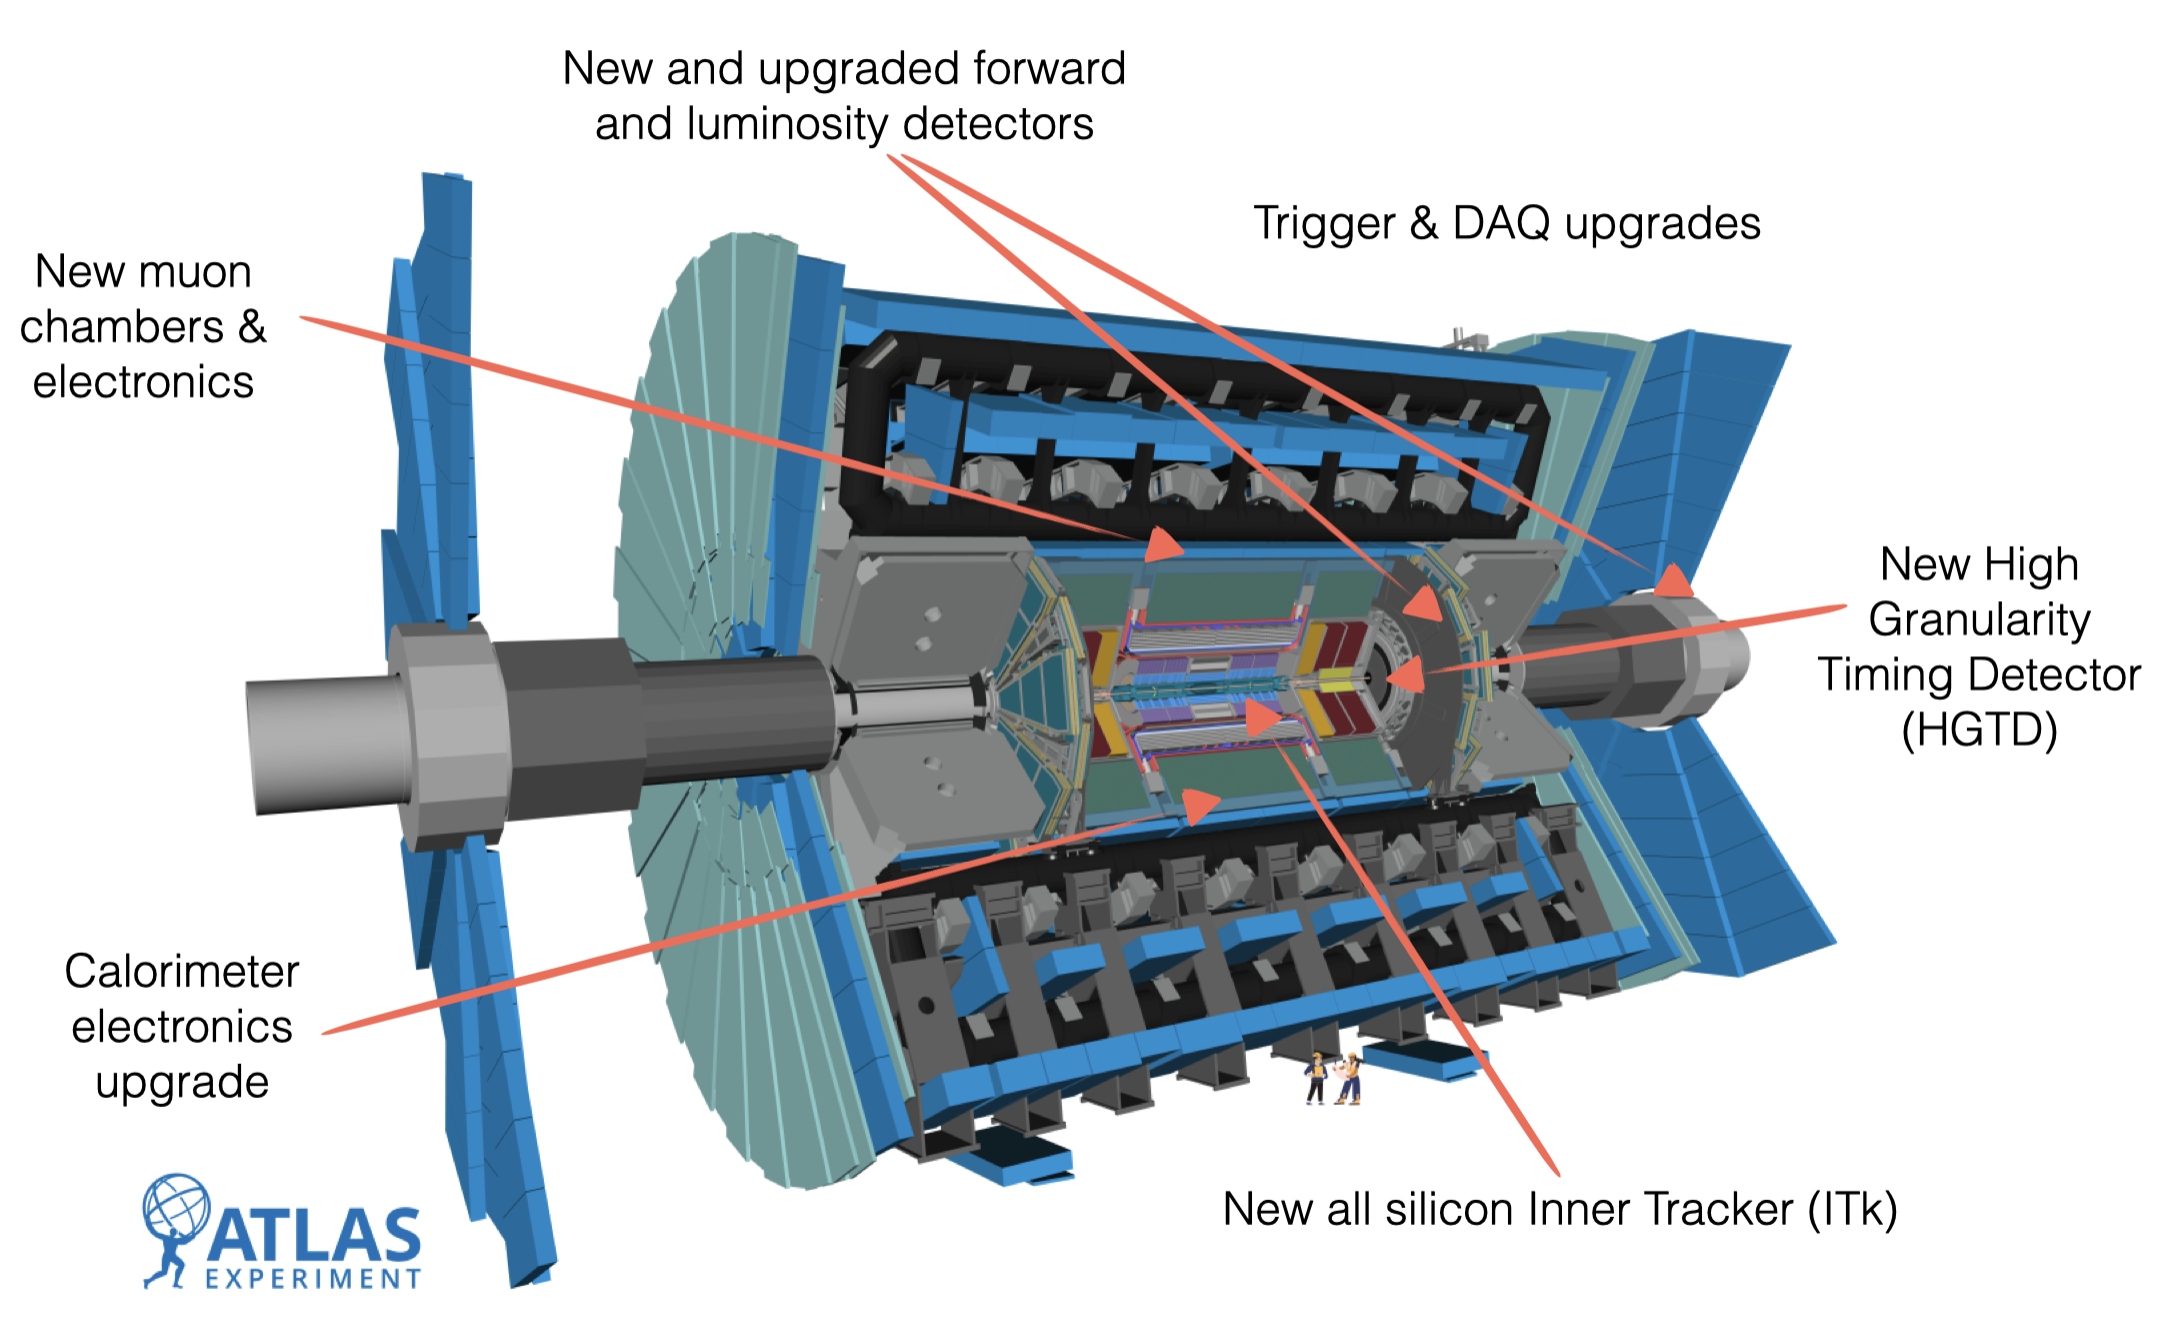
\includegraphics[width=0.98\linewidth]{figures/ch7-sMDT/ATLAS-upgrade.png}
    \caption{The ATLAS detector HL-LHC upgrade plan.}
    \label{fig:ATLAS-upgrade}
\end{figure}

The author of this thesis was extensively involved in the detector R\&D, construction, and testing of the muon small-diameter monitored drift tube (sMDT) chambers from 2019 to 2024 at the University of Michigan and at CERN. This chapter summarizes sMDT construction techniques and the author's major contributions, carried out in collaboration with a dedicated team of physicists, engineers, technicians, and students. 
%
These contributions include the design and development of the infrastructure, tooling, control systems, electronics, and software required for the construction and testing of sMDT tubes and chambers. The author also participated directly in the assembly of precision drift tubes and chambers, as well as in the execution of the associated quality-control tests. 
%
In addition, the author served as the primary author of two recent publications describing the construction and testing of the sMDT tubes and chambers~\cite{Wei:2022sMDTtube,Amidei:2023sMDTconstruction}. Detailed descriptions of the devices and instrumentation used in the sMDT construction at the University of Michigan can be found in these publications.


\section{sMDT tube construction and quality control tests}
\label{chap:sMDT-tube}
This section describes the design and construction of the infrastructure and test stations for small-diameter monitored drift tube (sMDT) assembly and testing, followed by the tube construction procedures, quality control tests, and their results.

The components of a precision sMDT tube and the overall tube geometry are shown in Figure~\ref{fig:sMDT-tube}(a) and (b), respectively. A critical component is the wire locator, known as the \textit{twister}, which holds the anode wire at the center of the tube with a precision better than $10~\mu\mathrm{m}$. The precision cylinder on the end-plug serves as the reference for the wire locator and is measured during chamber construction to determine the precise position of the wire.

\begin{figure}[!htb]
    \centering
    \subfloat[]{
    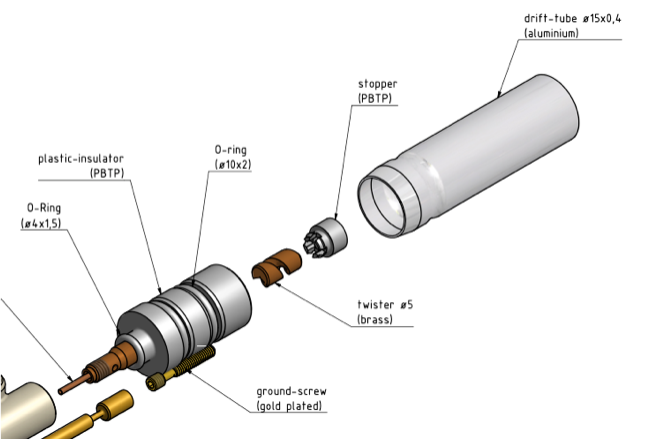
\includegraphics[width=0.42\linewidth]{figures/ch7-sMDT/end_plug1.png}
    }
    \subfloat[]{
    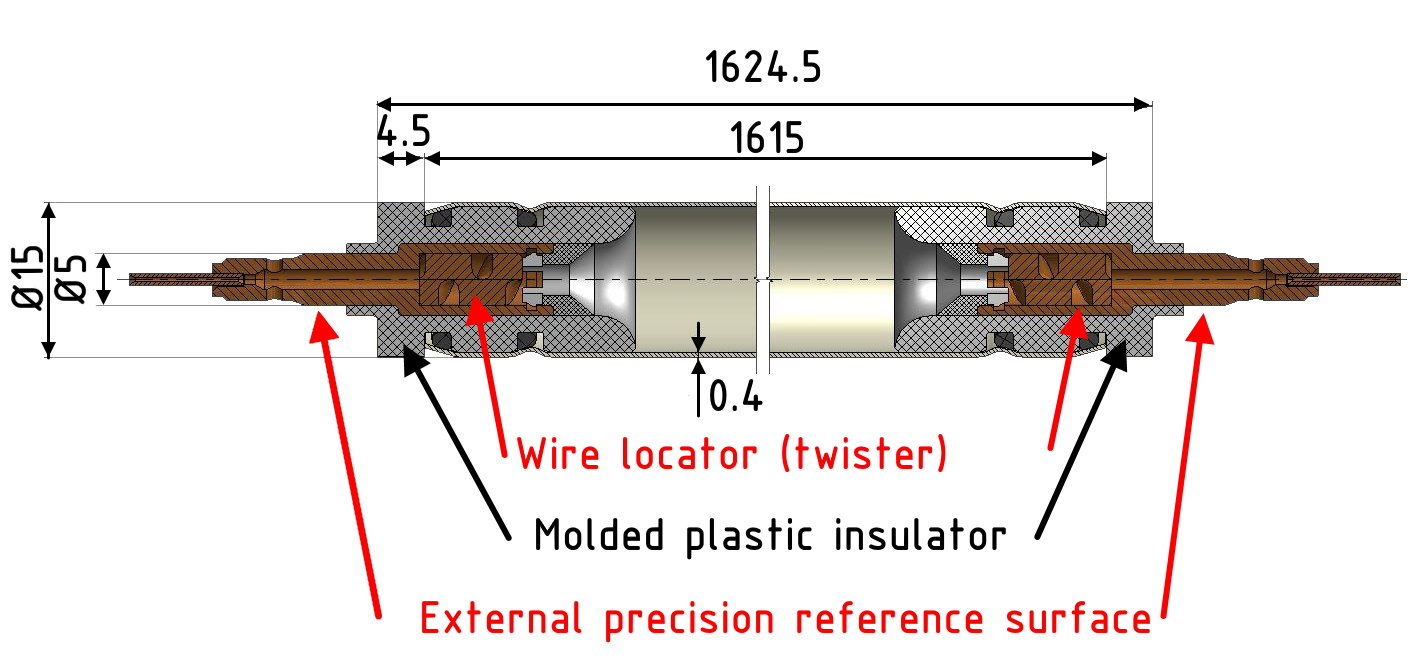
\includegraphics[width=0.57\linewidth]{figures/ch7-sMDT/TubeDesign_sBIS-1-6.jpg}
    }
    \caption{The small-diameter drift tube: left, components; right, cross-section view of an assembled end-plug and tube.}
    \label{fig:sMDT-tube}
\end{figure}

The sMDT drift tube design and parameters are described in 
detail in reference~\cite{ATLAS-TDR-026}.
Table~\ref{tab:parameters} lists the major tube parameters.
    \begin{table}[h]
        \centering
        \begin{tabular}{l|l}
             \hline
            Parameter & sMDT \\
            \hline
            Tube material & Aluminium AW6060-T6/AlMgSi \\
            Tube surface & Surtec 650 chromatization \\
            Tube outer diameter & 15.000 mm \\
            Tube wall thickness & 0.4 mm \\
            Tube length & 1615 mm \\
            Tube straightness & 0.5 mm / tube\\
            Wire material & W-Re (97:3) \\
            Wire diameter &  $50 \, \mu\mathrm{m}$ \\
            Wire resistance & 44 $\Omega$/m \\
            Wire tension & 350 $ {} \pm 15 \; $  g \\
            Gas mixture & Ar:CO2 (93:7) \\
            Gas pressure & 3 bar (abs.) \\
            Gas leak rate limit & $< ~ 1\times 10^{-8}~\frac{mbar ~\times ~cm^3}{sec}$ per tube\\
            Gas gain & $\rm 2\times10^{4}$ \\
            Wire potential & 2730 V \\
%            Maximum drift time & 180 ns \\
%            Wire positioning accuracy & $\rm 10\,\mu m$ r.m.s. \\
%            Wire dark current limit & $<$ 2 nA \\
            \hline
        \end{tabular}
        \caption{\rm sMDT tube materials and operating parameters}
        \label{tab:parameters} 
    \end{table}

\subsection{Stations for sMDT tube construction and testing}
\label{chap:stations}
The tube construction process consists of end-plug assembly, tube wiring, and crimping, as shown in the construction stations in Figure~\ref{fig:sMDT-stations}(a). 
\begin{figure}[!htb]
    \centering
    \subfloat[]{
    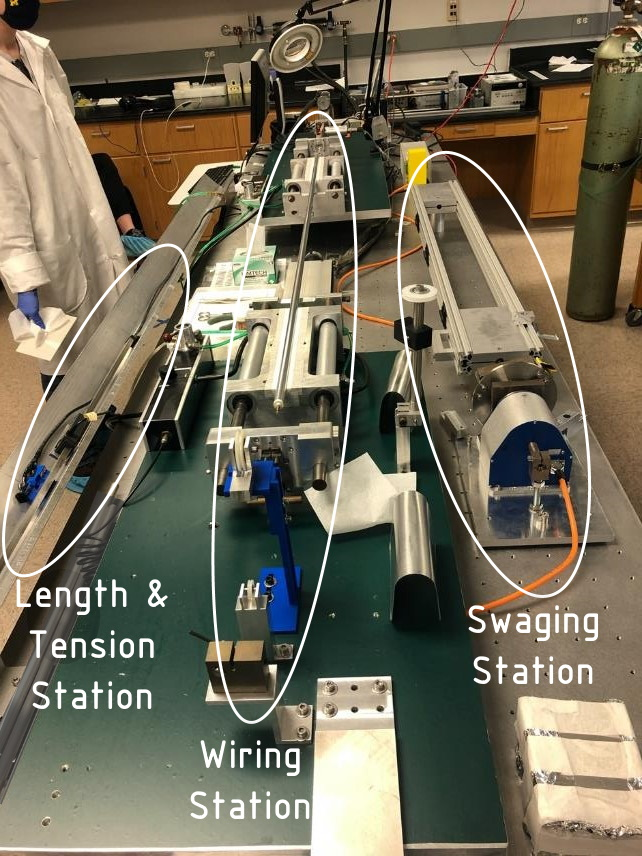
\includegraphics[width=0.49\linewidth]{figures/ch7-sMDT/wire-station-UM.jpg}
    }
     \subfloat[]{
    \includegraphics[width=0.49\linewidth]{figures/ch7-sMDT/tube-tension-test-station.png}
    }
    \caption{(a) The tube wiring and crimping stations, and (b) The wire tension and length measurement station.}
    \label{fig:sMDT-stations}
\end{figure}
The crimping step sets the wire tension and establishes a gas-tight seal between the end-plug and the inner wall of the tube. The quality control tests include measurements of the tube length, wire tension (see Figure~\ref{fig:sMDT-stations}(b)), gas leak rate, and dark current under a high voltage of 2730~V.

The wiring station consists of two vacuum chucks that hold the tube rigidly in a straight line and aligned with the wire feed. The wire is supplied from a spool mounted on a magnetically damped spindle to allow smooth pulling, and passes through a tube and through a three-wheel tension meter and a linear actuator, as shown in Figure~\ref{fig:sMDT-wire-tension}(a), which stretches the wire to the desired tension of 350~g. Two pairs of cam-operated crimp jaws (see Figure~\ref{fig:sMDT-wire-tension}(b)) are mounted at each end of the chuck. These jaws compress the 1.0~mm outer-diameter wire-crimping tube down to 0.7~mm, thereby fixing the wire tension inside the tube.
\begin{figure}[!htb]
    \centering
    \subfloat[]{
 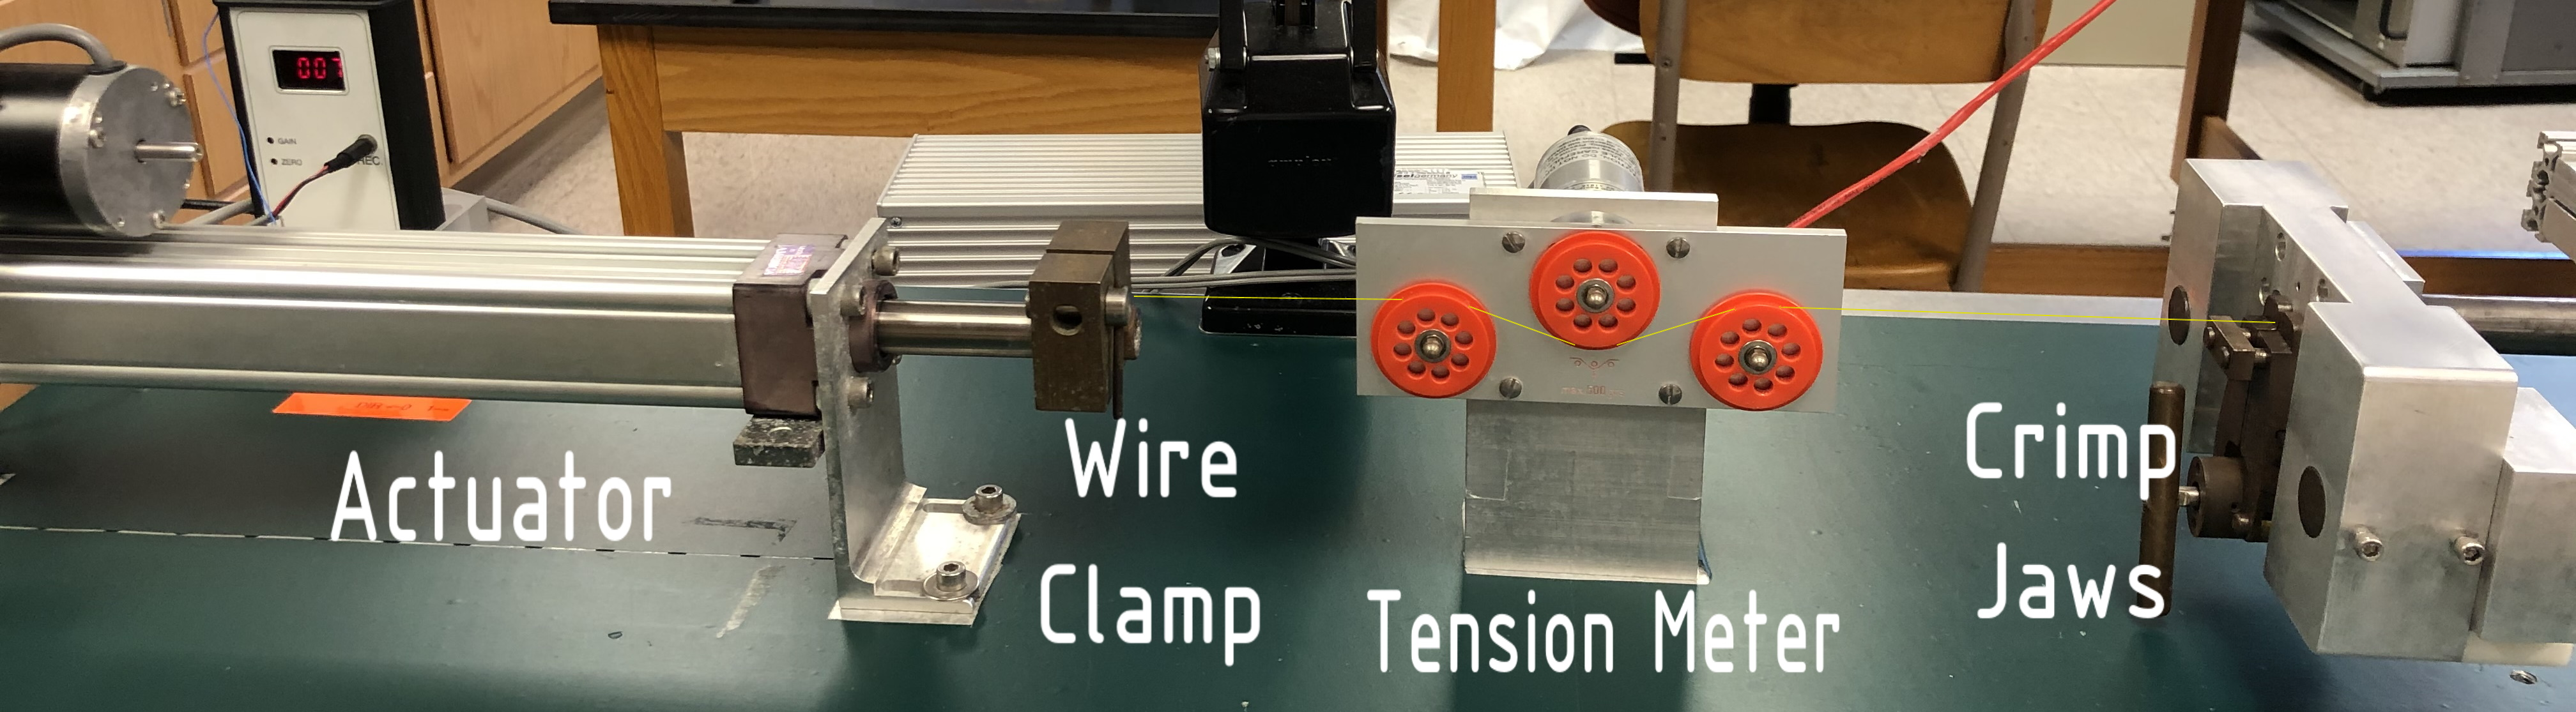
\includegraphics[width=0.72\linewidth]{figures/ch7-sMDT/WireTensionGauge2a.jpg}
 }
 \subfloat[]{
    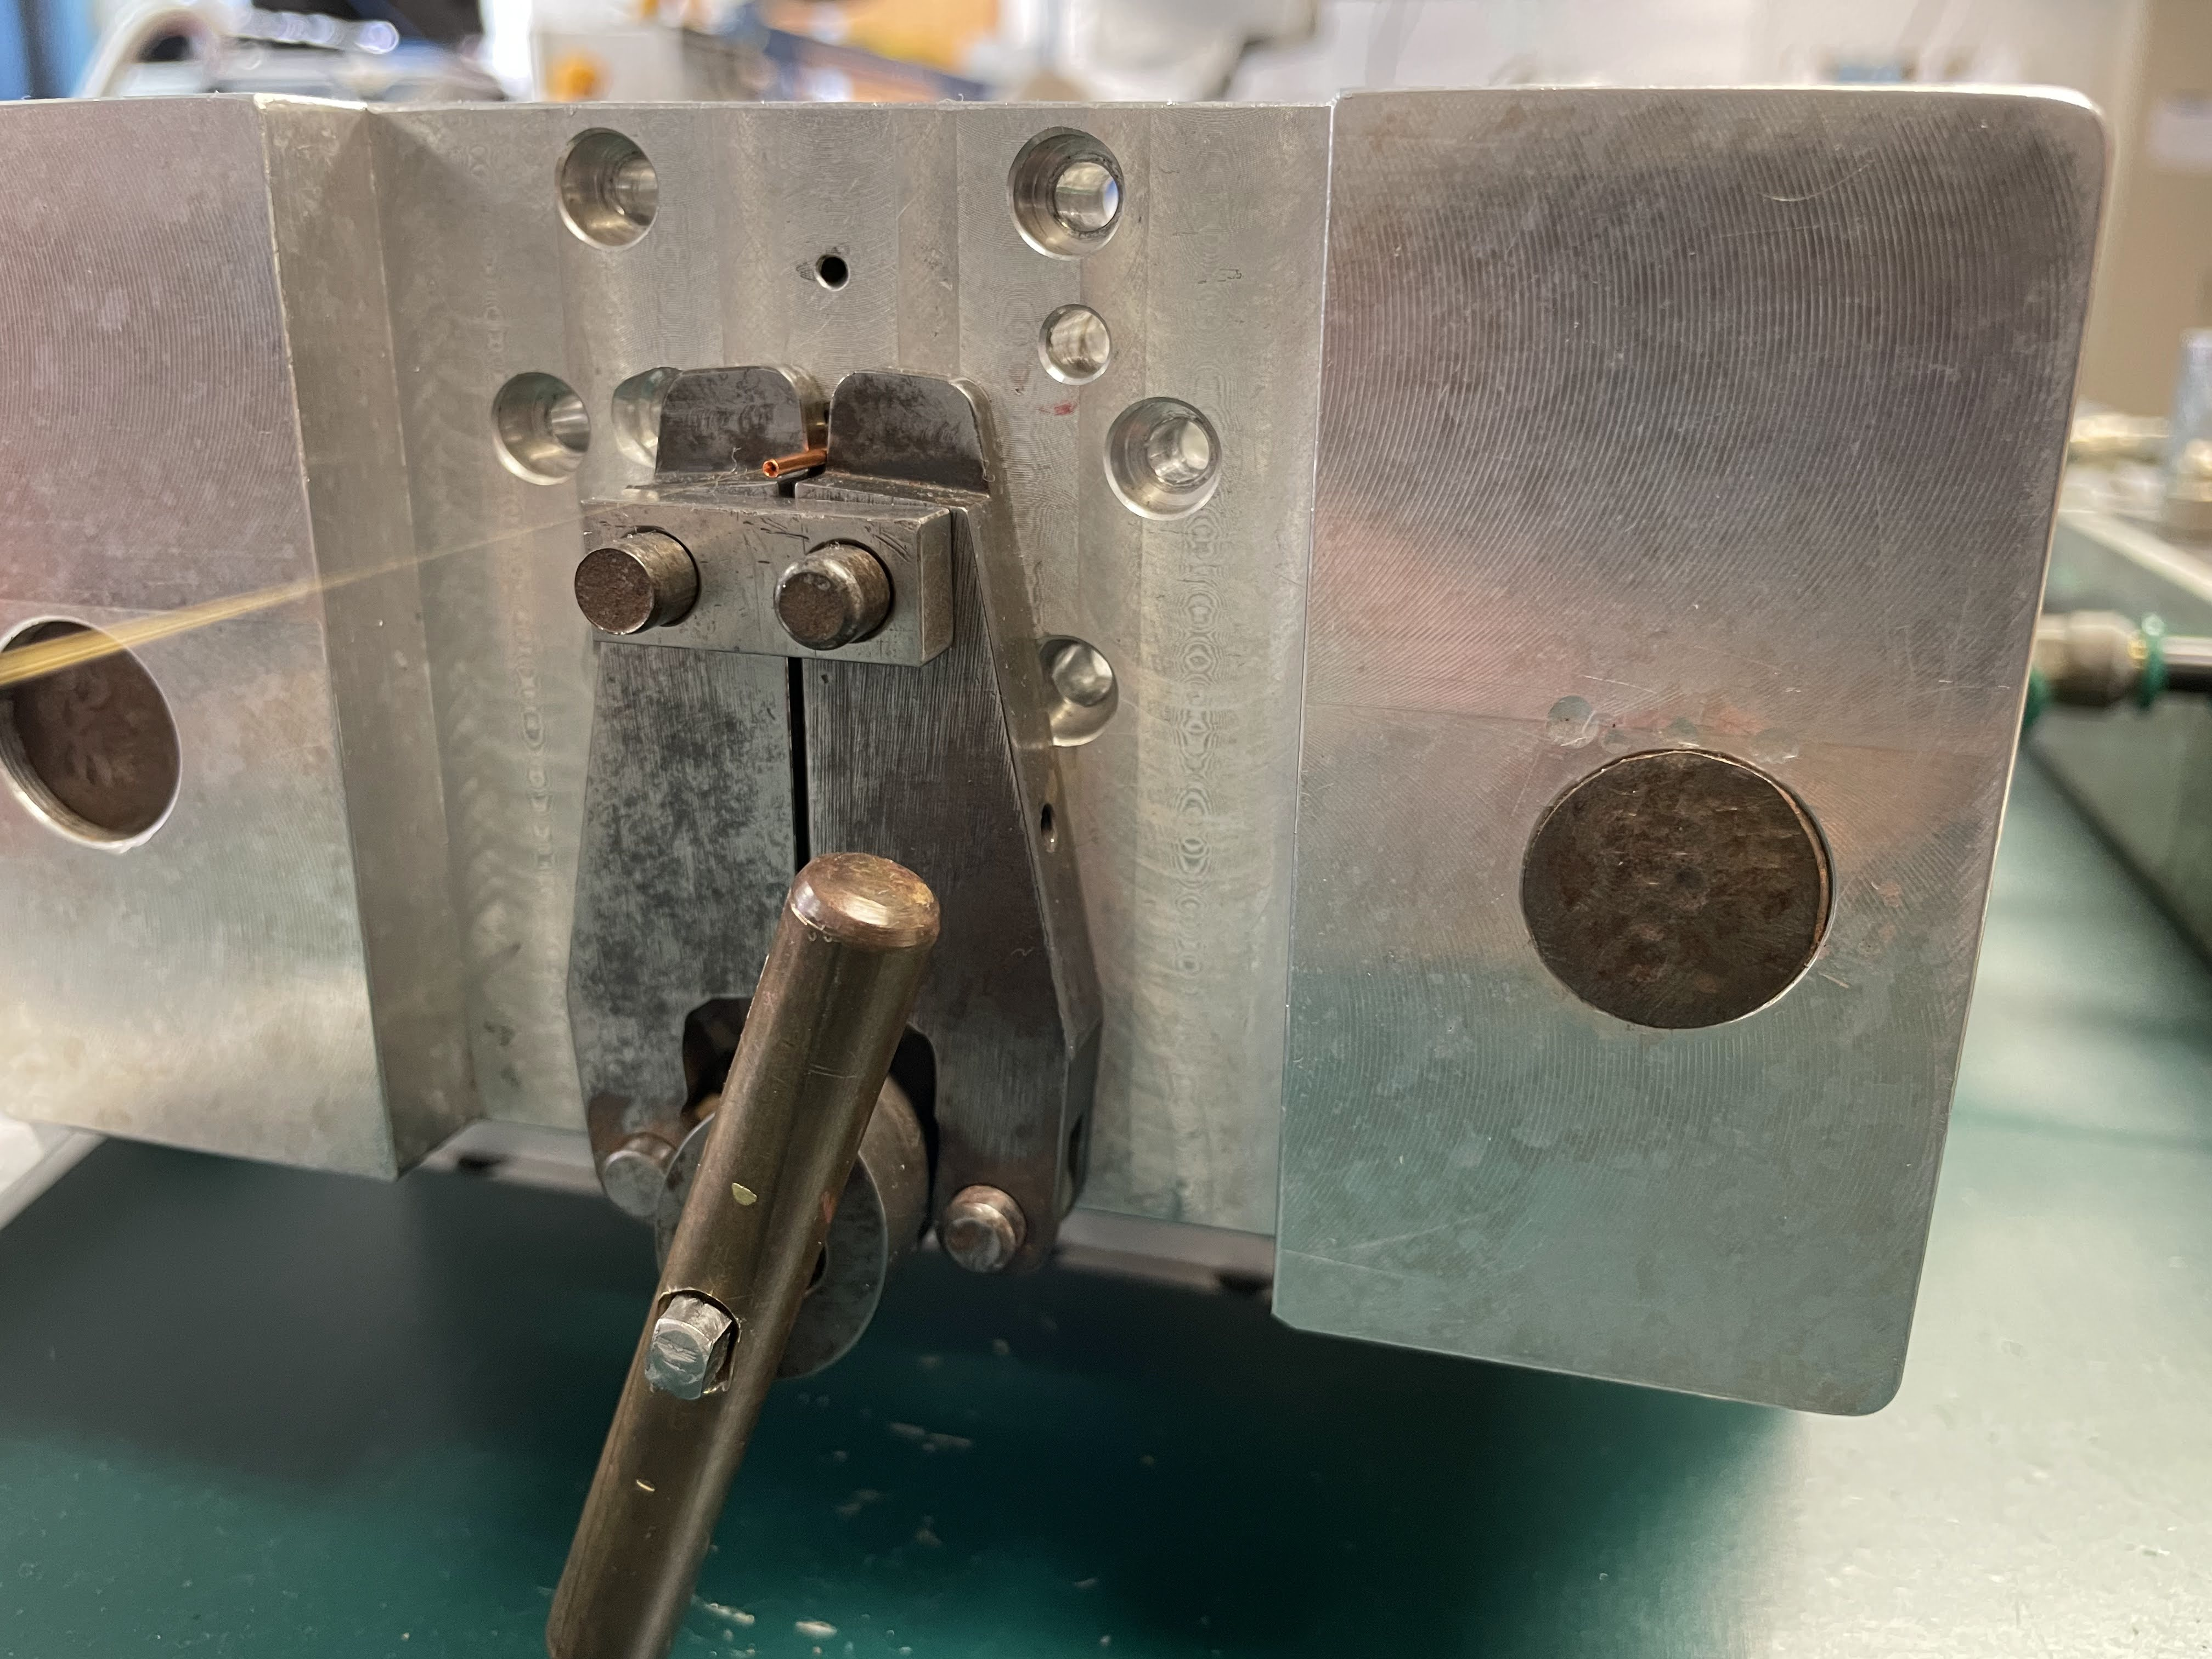
\includegraphics[width=0.27\linewidth]{figures/ch7-sMDT/CrimpJaws.jpg}
    }
    \caption{(a), Wire tension gauge. (b), wire crimping jaw.}
    \label{fig:sMDT-wire-tension}
\end{figure}

The second station used in tube construction is the tube crimping station, where the thin wall of the tube is deformed (crimped) to compress against the O-rings on the end-plugs and form a gas-tight seal. The crimping head is a custom-built rotary device
that gradually forces three roller heads radially inward while rotating
around the tube. The side view and end view of the rotator setup are shown
in Figure~\ref{fig:sMDT-tubeswage}(a) and (b), respectively.
\begin{figure}[!htb]
    \centering
        \subfloat[]{
 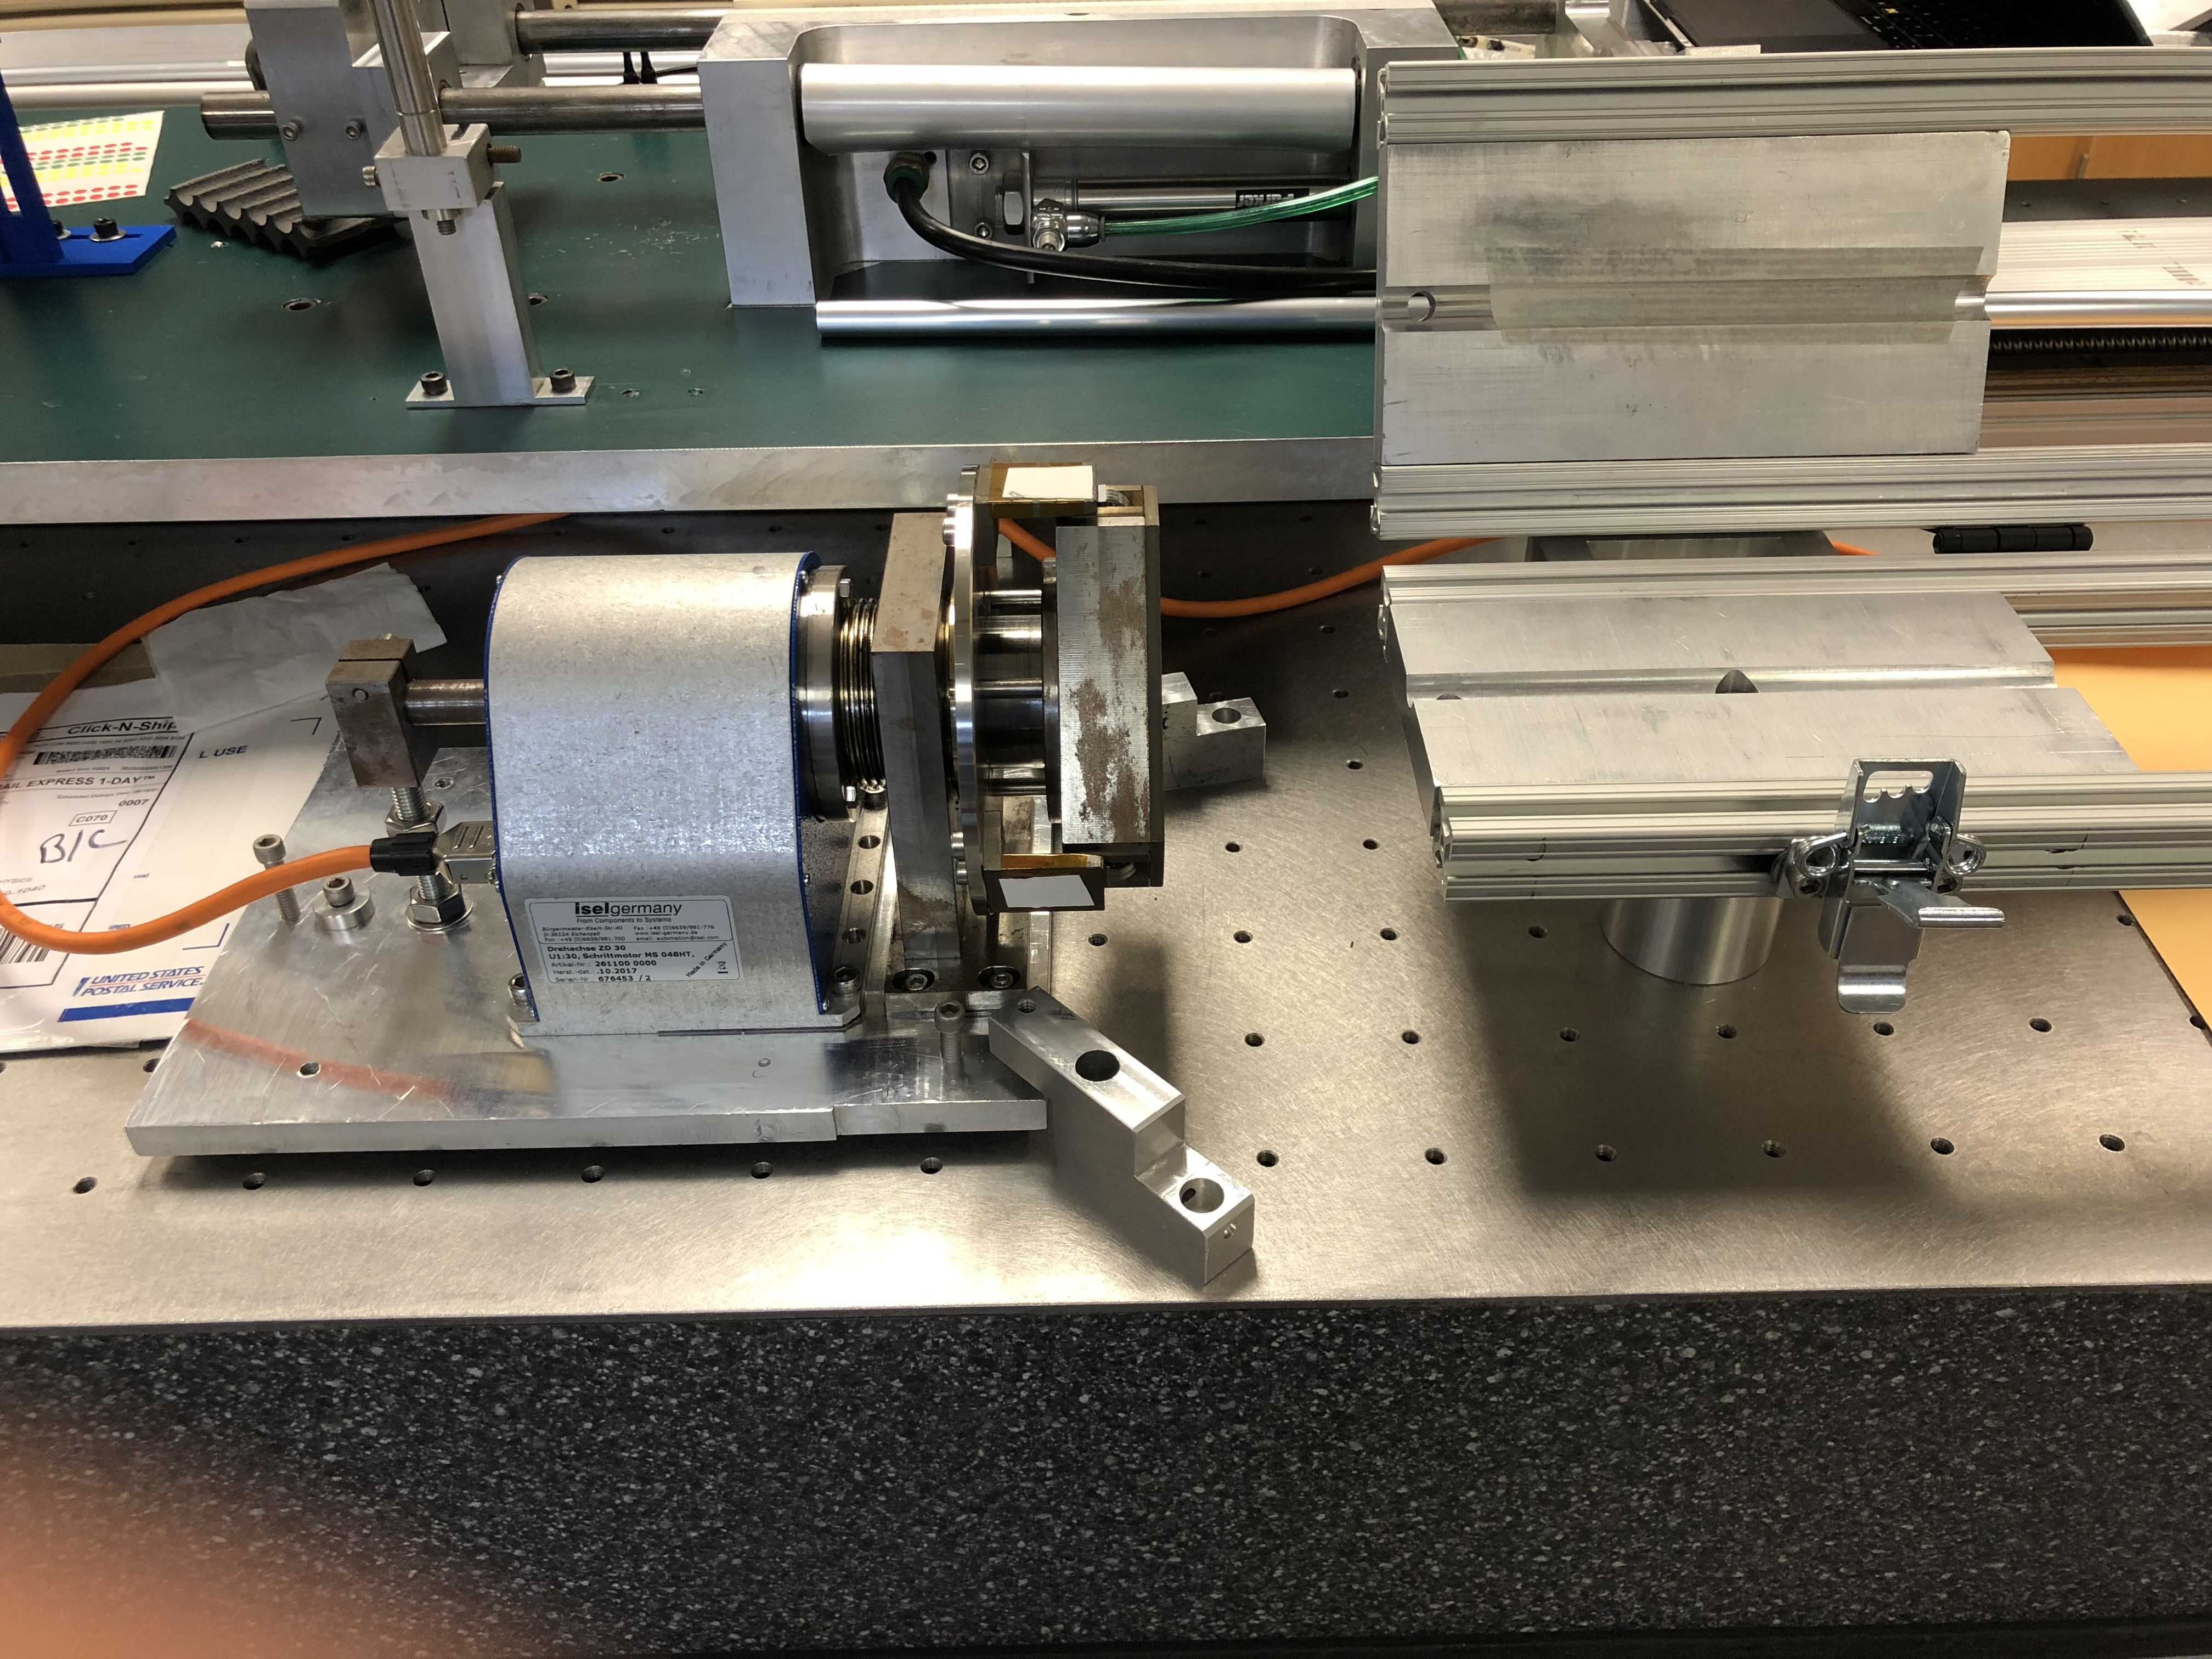
\includegraphics[width=0.48\linewidth]{figures/ch7-sMDT/SwagerSideView.jpg}
 }
     \subfloat[]{
    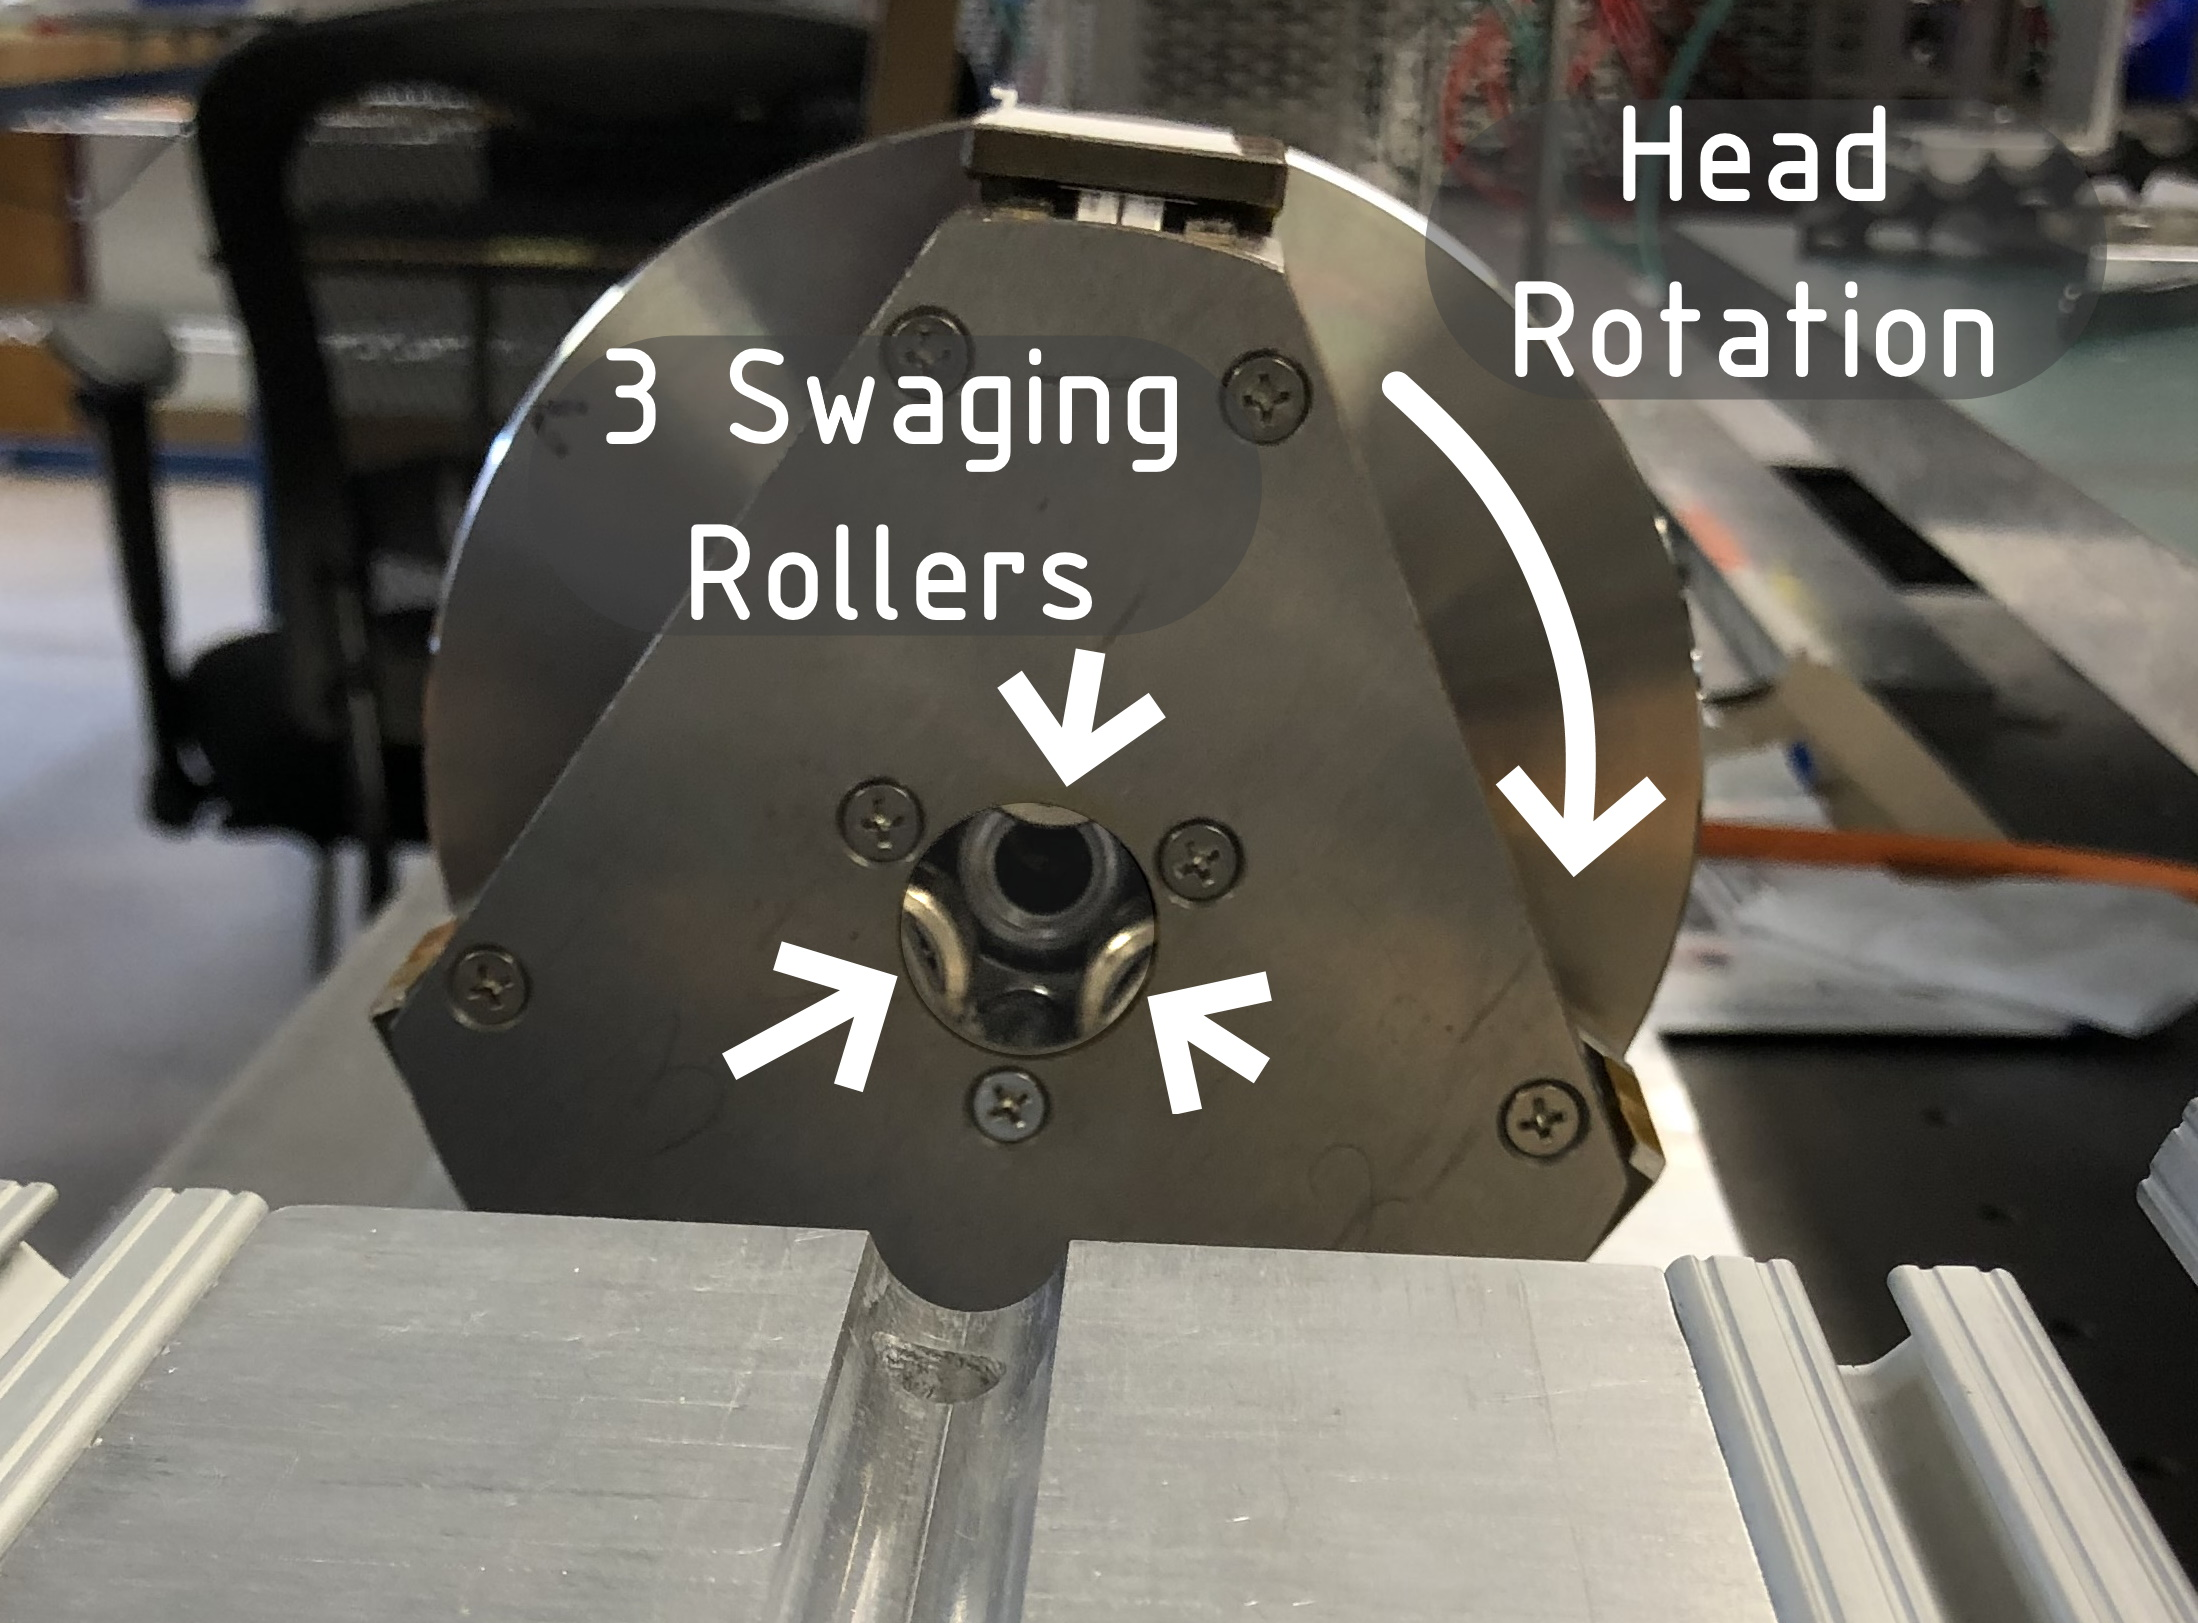
\includegraphics[width=0.49\linewidth]{figures/ch7-sMDT/SwagerEndView-a.jpg}
 }
    \caption{Tube crimping set up, (a) side-view and (b) the end-view.}
    \label{fig:sMDT-tubeswage}
\end{figure}

The wiring and tube-crimping control software were developed by the author of this thesis using LabVIEW~\cite{LabView} framework to operate the linear actuator and the rotator motor. During the wiring process, the program continuously monitors the wire tension using the tension gauge while the wire is being pulled. The wire is first stretched to a tension of 400~g and held at this level for one minute, after which the tension is relaxed to the final value of 350~g. The wire is then fixed by crimping with the crimping jaws. This procedure ensures a stable final wire tension.
%
For the tube crimping required to achieve the gas seal, the motor controls both the rotation and the forward motion of the crimping head. During this process, the three crimping (swaging) rollers are gradually pushed inward at the O-ring locations, compressing the tube wall against the O-rings to form a gas-tight seal. After the crimping is completed, the motor moves backward to retract the rollers to their original radial positions, allowing the tube to be released from the rotating head.

After the tube is crimped, the tube assembly is complete. The tube is then immediately subjected to a gas leak test. The leak test station, designed and constructed as shown in Figure~\ref{fig:sMDT-leaktest}(a), consists of a helium mass spectrometer leak detector connected to a vacuum vessel with an inner diameter of 25~mm and a length of 1.8~m. 
%
During the test, one end of the tube is sealed with a brass cap and an O-ring, while the other end is screwed into the cap of the vacuum vessel, allowing the tube to be pressurized with helium at 3~bar. The constructed tube is required to be leak-tight with an upper leak-rate limit of $\rm 1\times10^{-8}\,cm^{3}\,mbar/s$ at a tube pressure of 3~bar (absolute).
\begin{figure}[!htb]
    \centering
        \subfloat[]{
 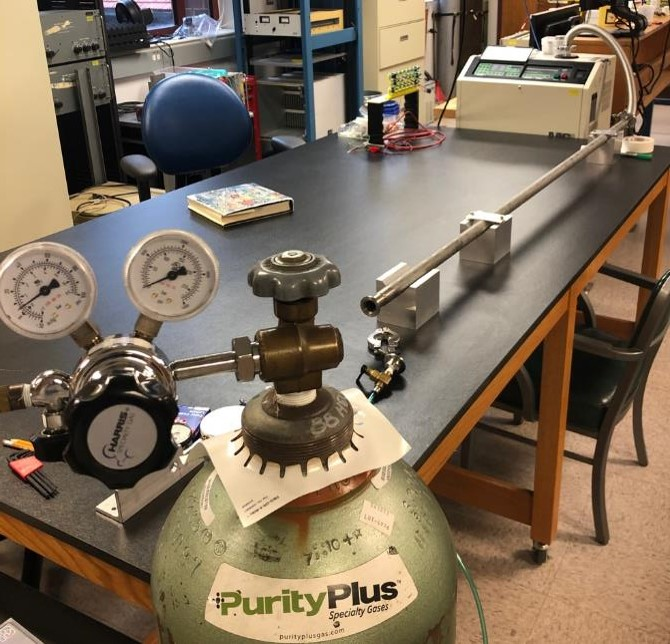
\includegraphics[width=0.43\linewidth]{figures/ch7-sMDT/leak-test-station.jpg}
 }
     \subfloat[]{
  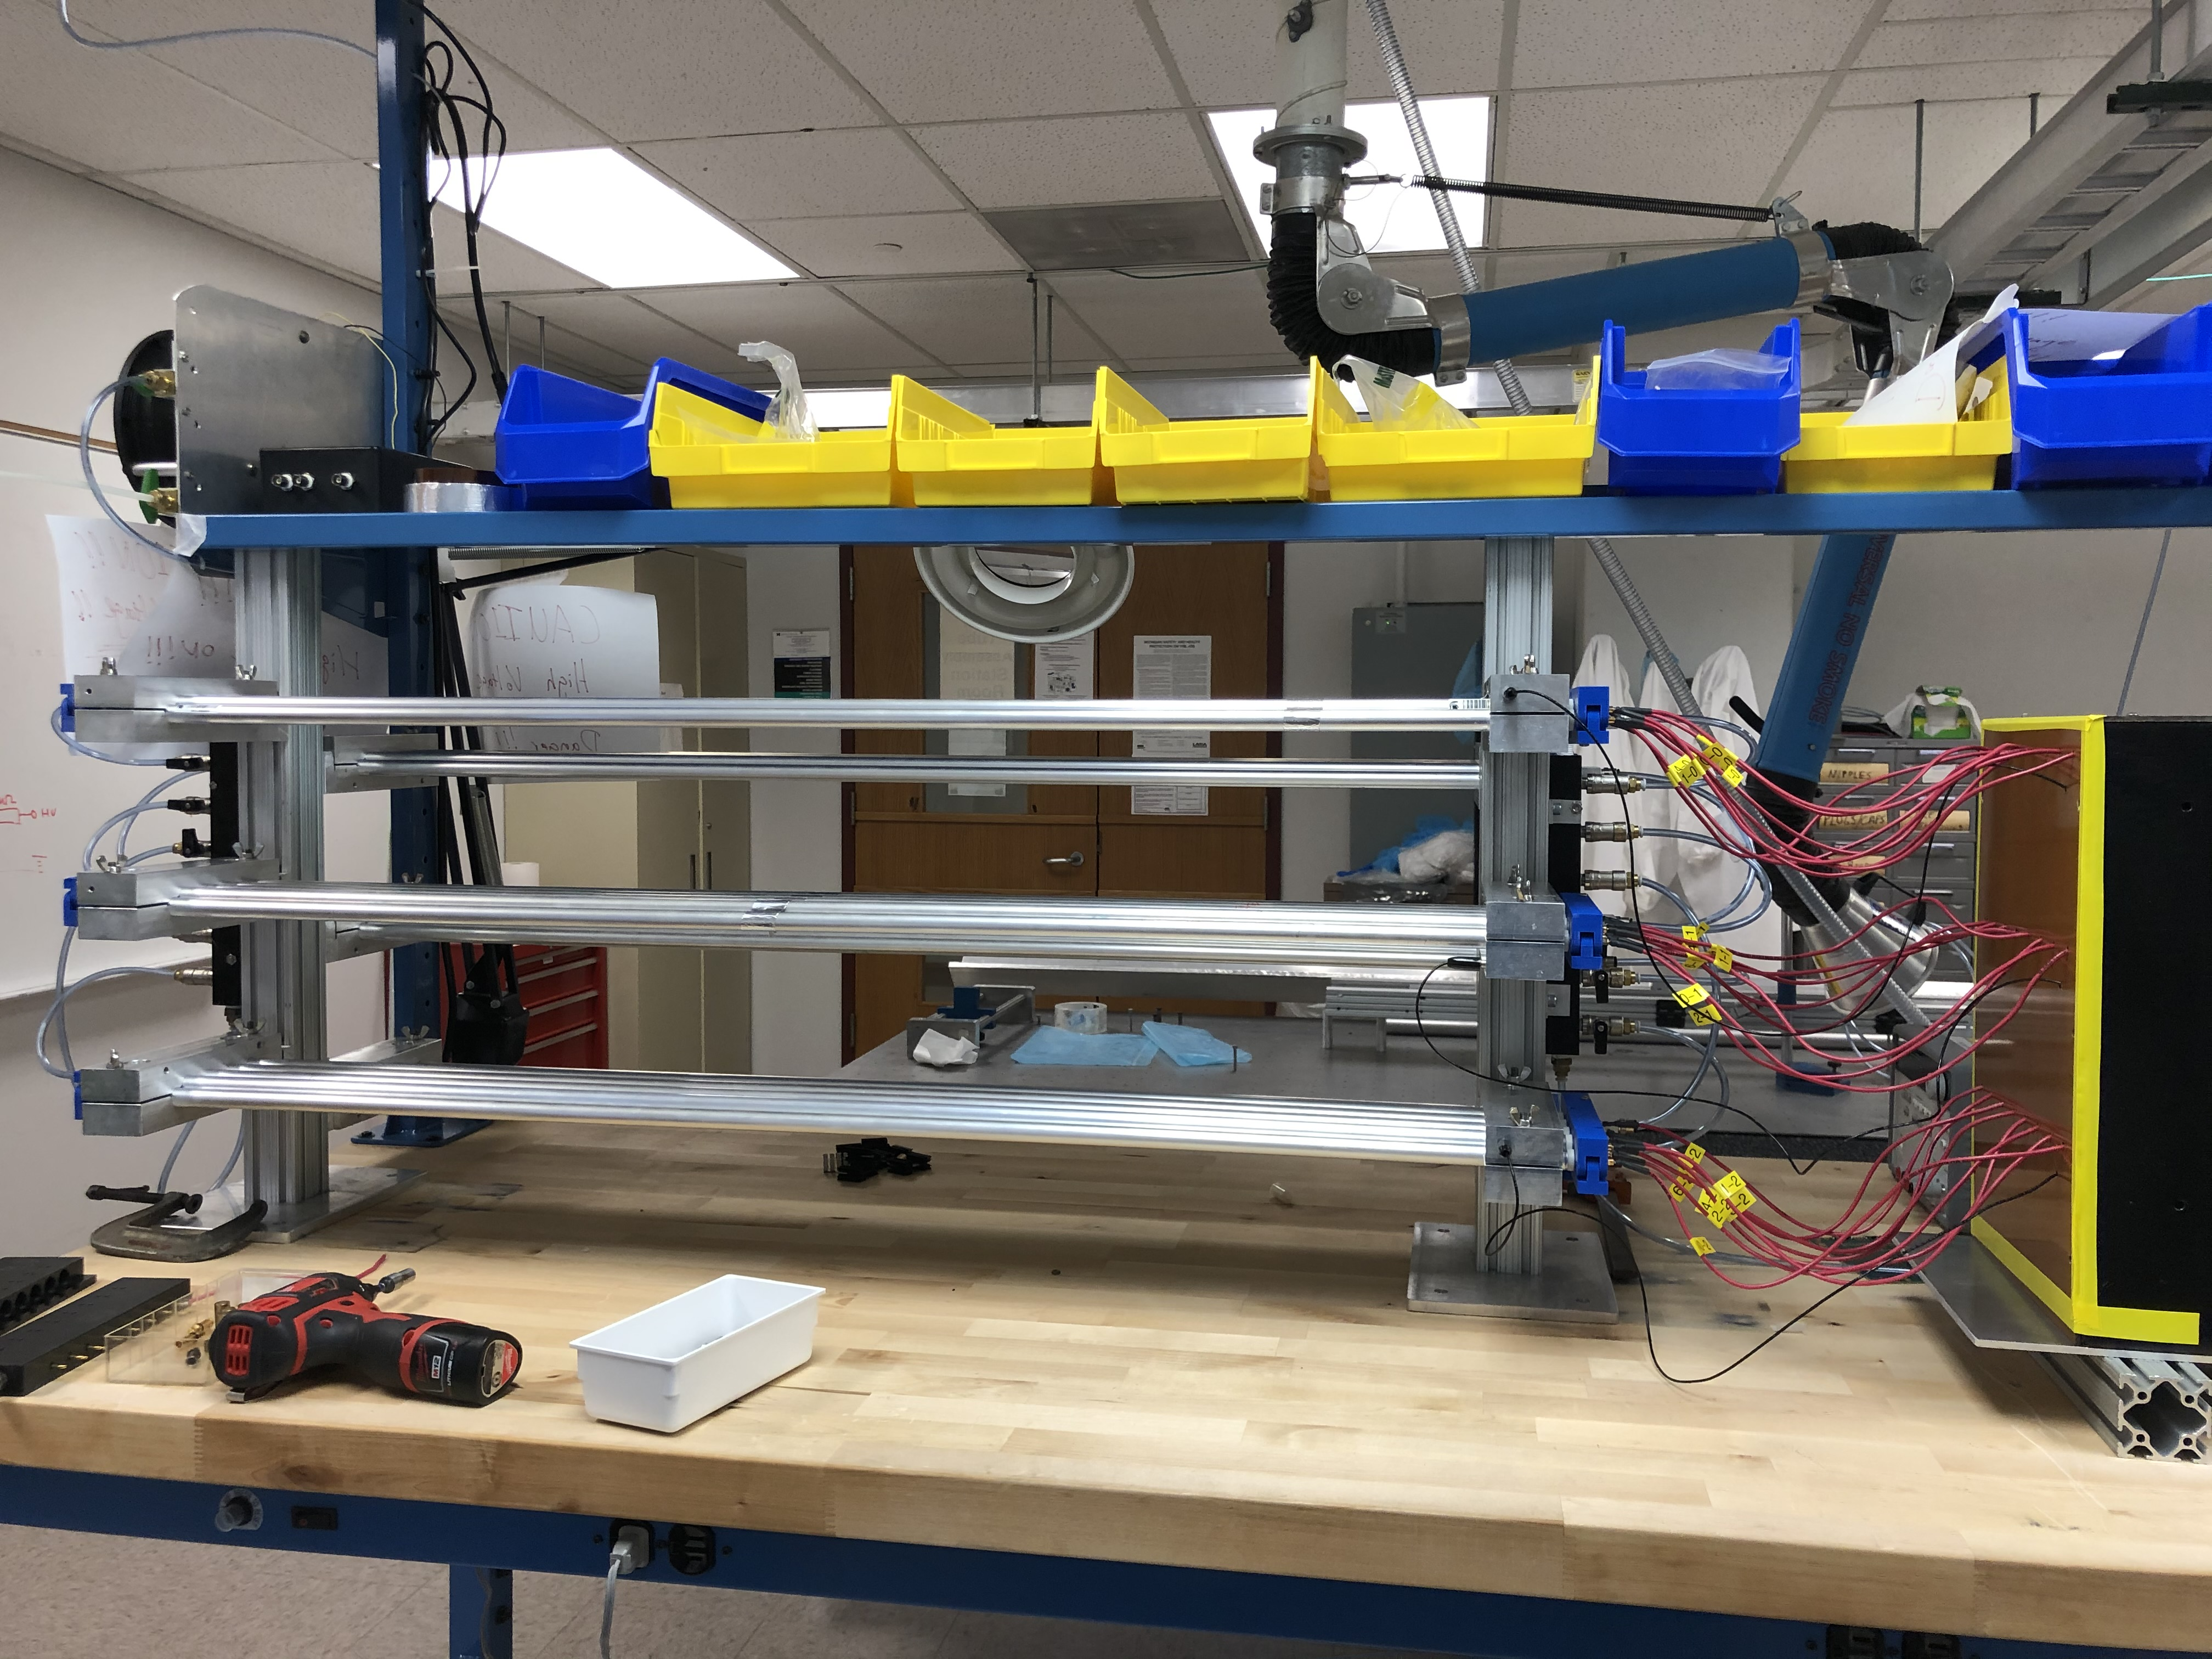
\includegraphics[width=0.55\linewidth]{figures/ch7-sMDT/DC-Test-Station.jpeg}
  }
    \caption{(a)Tube leak test station. (b)Dark-current test station. }
    \label{fig:sMDT-leaktest}
\end{figure}

Figure~\ref{fig:sMDT-leaktest}(b) shows the tube dark current test station, which consists of a gas flow control panel, custom-built dark current test electronics, HV/LV power systems, and an online monitoring and data acquisition system capable of testing 24 tubes in parallel. The author of this thesis designed and set up the front-end electronics and developed the online DAQ software for this test station.

\begin{figure}[!htb]
    \centering
 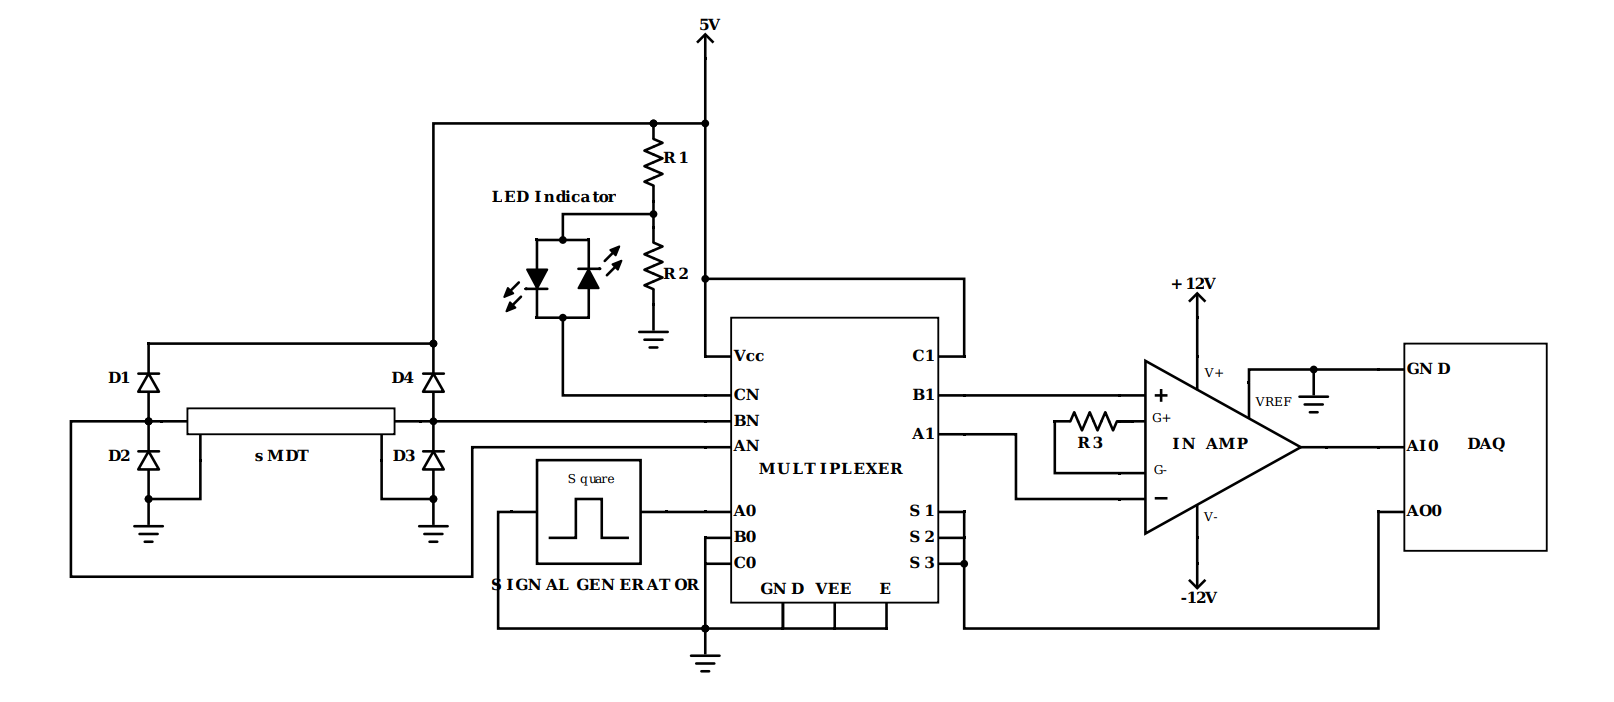
\includegraphics[width=0.95\linewidth]{figures/ch7-sMDT/Circuit-Tension-Test.PNG}
    \caption{Schematic of wire tension test circuit. }
    \label{fig:sMDT-circuit}
\end{figure}

The tube length and the wire tension are measured 
using the station shown in Figure~\ref{fig:sMDT-stations}(b).
A tube is placed in the V-shaped aluminum bar with its 
midpoint inside a U-shaped magnet, and a linear digital scale is used for the length measurement. 
%
Wire tension is measured using the same setup. The aluminum tube is grounded on a V-shaped support, while the wire is connected to a custom multiplexing circuit (Figure~\ref{fig:sMDT-circuit}) consisting of an analog multiplexer, a signal generator, an instrumentation amplifier, and the tube itself. A pulse from the signal generator excites wire vibrations, and the resulting signal is amplified and recorded by a data acquisition (DAQ) system interfaced with a computer. A graphical user interface was developed to set measurement parameters (e.g., tube length) and perform real-time analysis.

After the excitation pulse stops, the wire oscillates at its natural frequencies~\cite{TensionPaper}:
\begin{equation}
  f_n = \frac{n}{2L}\sqrt{\frac{T}{\rho}},
  \label{eq:tension}
\end{equation}
where $L$ is the wire length, $T$ the tension, and $\rho$ the wire density. The tension can be expressed as
\[
T = \frac{\pi L^2 d^2 f_1^2 \rho}{g}.
\]
For the nominal sMDT parameters ($L = 1597$~mm, $d = 50~\mu$m, $\rho = 19.7~\mathrm{g/cm^3}$, $g = 9.81~\mathrm{m/s^2}$), the first resonant frequency of 93.3~Hz corresponds to a wire tension of 350~g. The resonant frequency is extracted using a custom LabVIEW program that applies a fast Fourier transform (FFT) to determine $f_1$ and thus the wire tension.

%%%%%%%%%%%%%%%
\subsection{sMDT tube construction and quality control test results}
\label{chap:asembling-tubes}
Using the tube construction and test stations described in Section~\ref{chap:stations}, and following the well-established procedures outlined above, approximately 3,500 (22,000) precision drift tubes were constructed at the University of Michigan (Michigan State University). All 26,000 tubes were fully tested at the University of Michigan (UM). 

The overall failure rate of the tubes produced at UM was below 3\%, based on the quality control test criteria. Figure~\ref{fig:sMDT-length-tension-dc} presents the tube production quality control results for tube length (a), wire tension (b), and dark current (c), demonstrating the excellent quality of the tubes produced for sMDT chamber construction in the ATLAS HL-LHC upgrade project.

\begin{figure}[!htbp]
    \centering
        \subfloat[]{
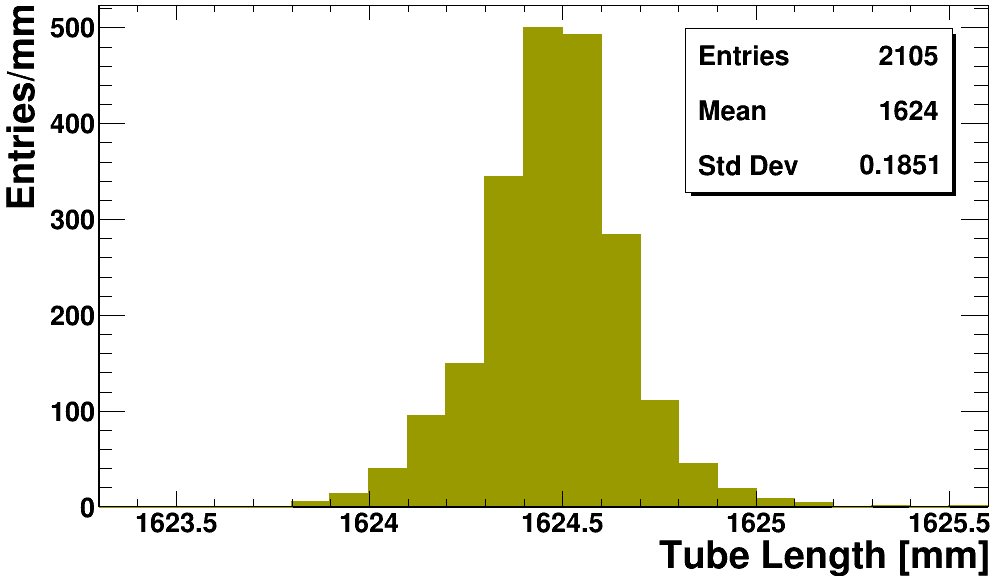
\includegraphics[width=0.37\linewidth]{figures/ch7-sMDT/UM_LEN.png}}
    \subfloat[]{
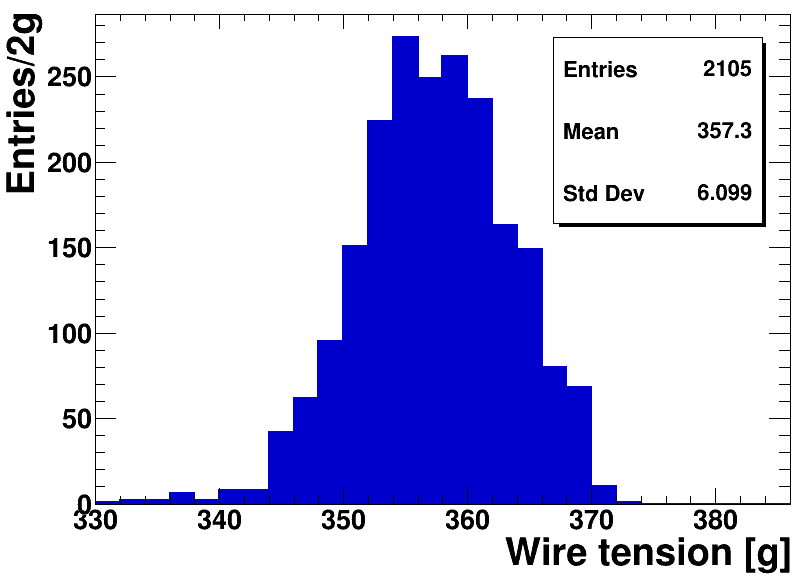
\includegraphics[width=0.31\linewidth]{figures/ch7-sMDT/UM_TEN.png}}
    \subfloat[]{
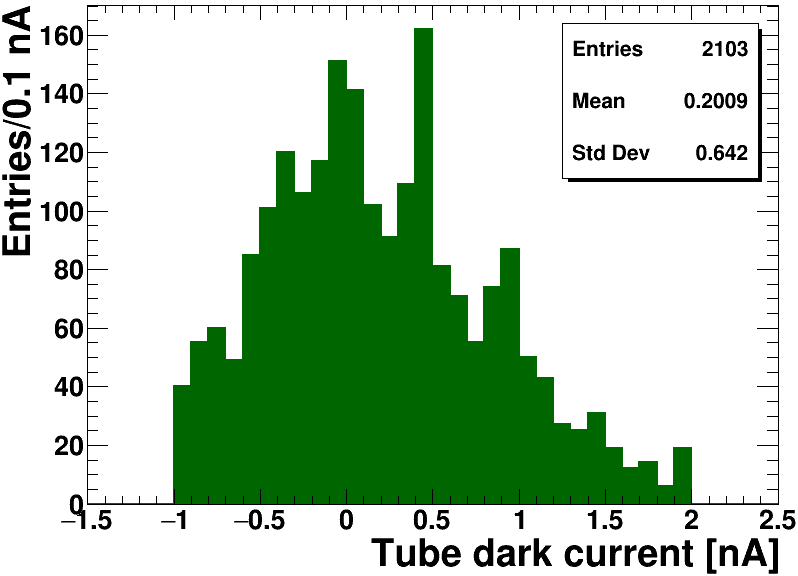
\includegraphics[width=0.30\linewidth]{figures/ch7-sMDT/UM_DC.png}}
\caption{Tube production quality control test results on tube length (a), wire tension (b), and dark-current (c). }
    \label{fig:sMDT-length-tension-dc}
\end{figure}

\begin{figure}[!htb]
    \centering
     \subfloat[]{
  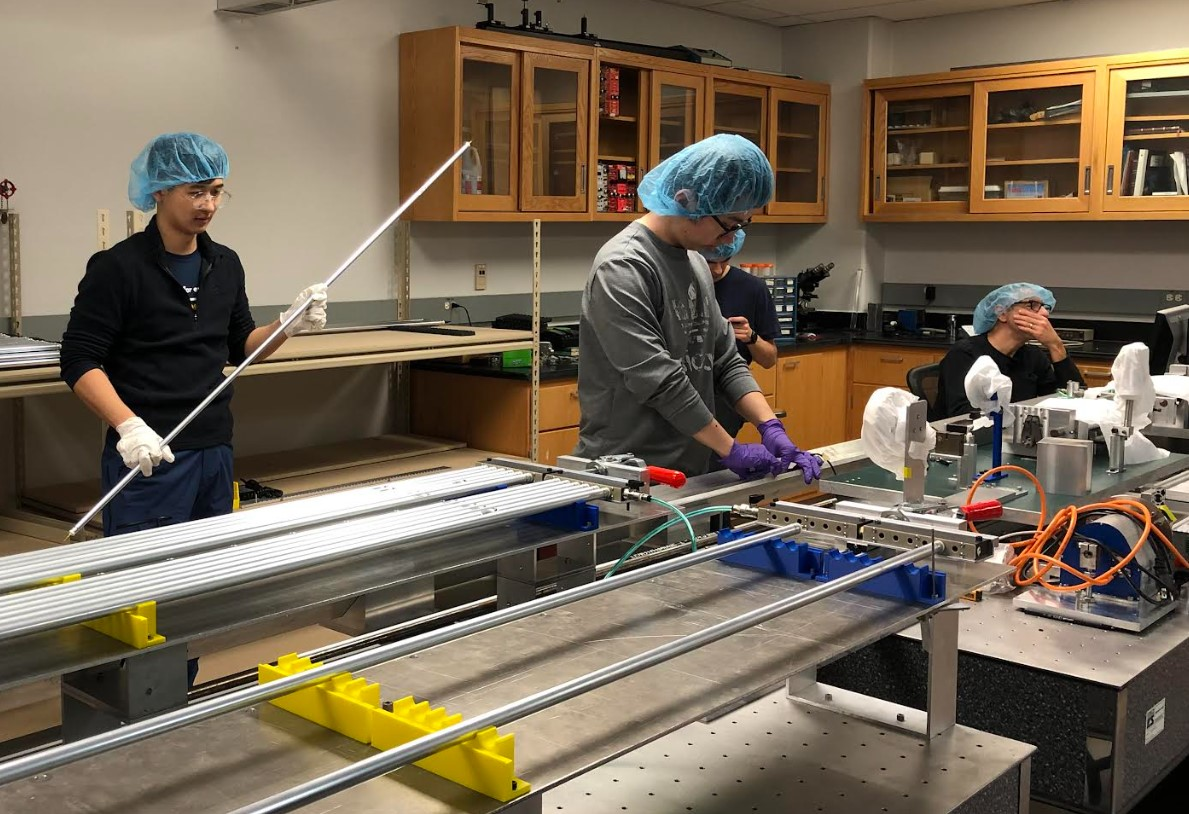
\includegraphics[width=0.48\linewidth]{figures/ch7-sMDT/Tube-test.jpg}
  } \hspace{0.3cm}
      \subfloat[]{
    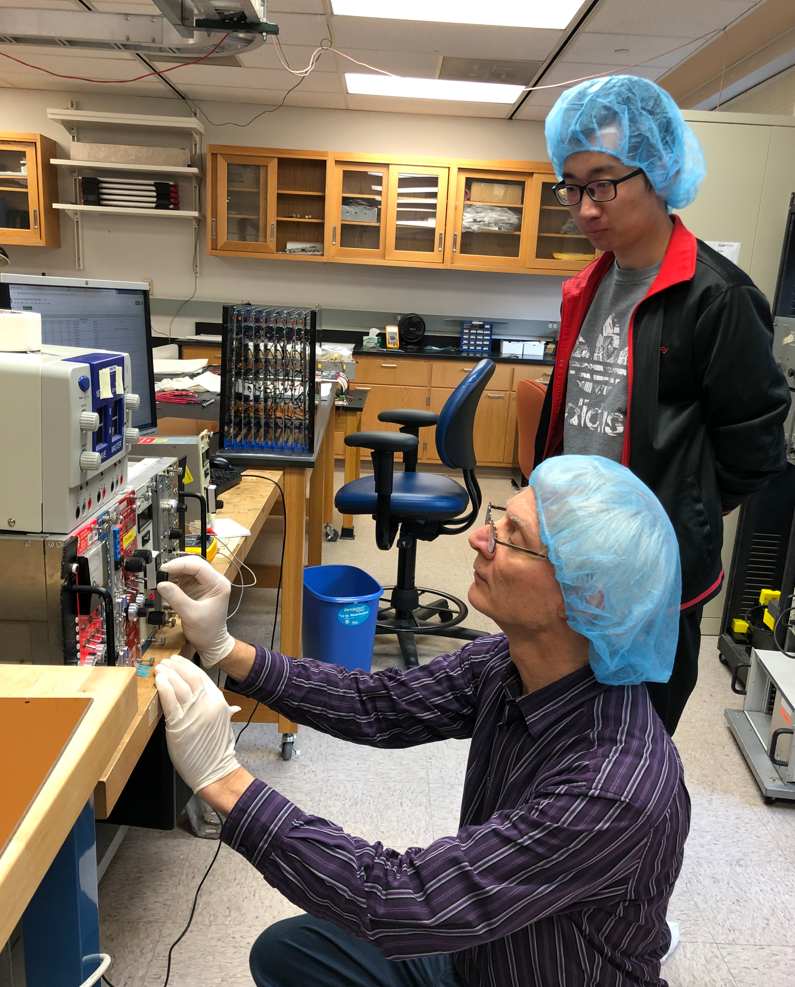
\includegraphics[width=0.265\linewidth]{figures/ch7-sMDT/chuanshun-Curtis.png}
 }
    \caption{(a) sMDT tube construction and wire tension measurement performed by the author of this thesis (center) together with two students. (b) Set up and testing of the dark current test station by an engineer and the author.}
    \label{fig:sMDT-test-setup}
\end{figure}

The large-scale sMDT tube construction and testing effort at the UM was carried out primarily by a student team. The author's major contributions include building the dark-current test electronics boards and setting up and debugging the workstation hardware and software. Figure~\ref{fig:sMDT-test-setup}(a) shows the author (center) performing sMDT tube construction and wire tension measurements with two students, while Figure~\ref{fig:sMDT-test-setup}(b) shows the author and an engineer setting up and testing the dark-current station.


%\subsection{sMDT tube Assemb}

%\subsection{sMDT tube Quality Test}

%\subsubsection{Straightness}

%\subsubsection{Gas Tightness}

%\subsubsection{Dark Current}

%\subsubsection{Tension}
\clearpage

%-------------Chamber----------------

\section{sMDT chamber construction}
\label{chap:sMDT-chamber}

The fully tested sMDT tubes are assembled into larger structures known as chambers. 
\begin{figure}[!htb]
    \centering
 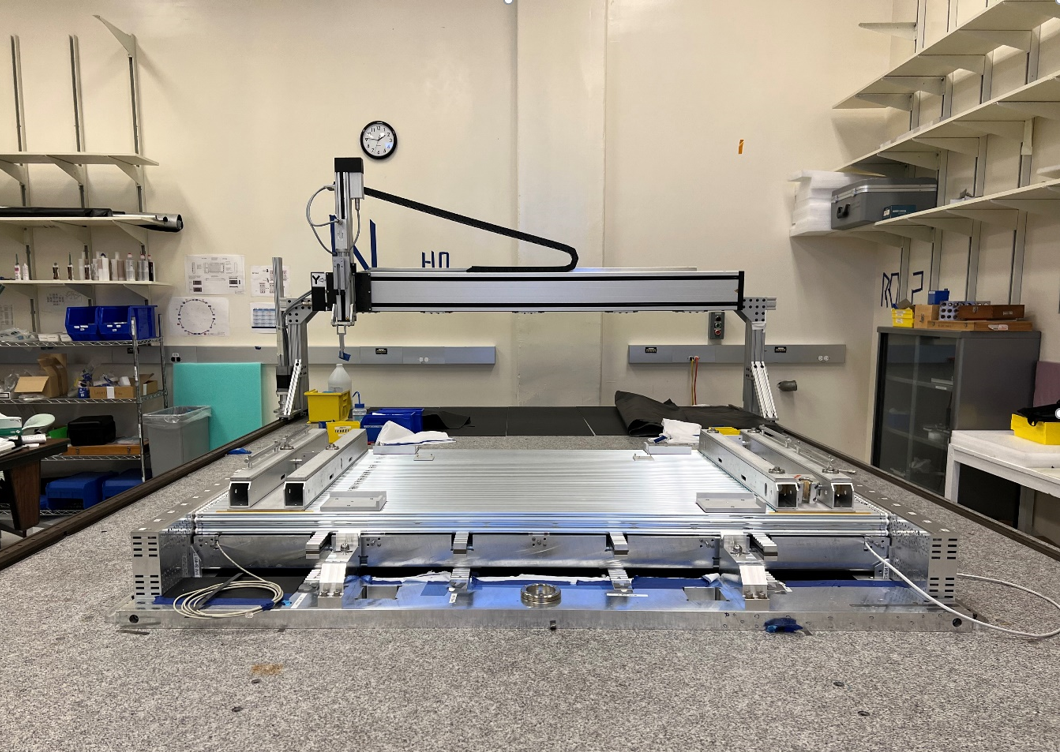
\includegraphics[width=0.95\linewidth]{figures/ch7-sMDT/chamber-on-granite.PNG}
    \caption{A constructed chamber on the assembly jig, mounted on a large granite table.}
    \label{fig:sMDT-chamber-granite}
\end{figure}
Figure~\ref{fig:sMDT-chamber-granite} shows 
a reconstructed sMDT chamber still held by the precision construction combs at both ends of the chamber on the large flat granite table, and the automatic glue machine, which was parked at the end of the granite table.

The chamber consists of two tube multilayers (MLs), each containing four tube layers of 70 tubes (BIS1) or 58 tubes (BIS2--6). A spacer frame containing the optical in-plane alignment system is glued between the two MLs. Platforms for mounting the magnetic-field sensors and global alignment devices are attached on top of the chamber, together with the chamber kinematic mounts used to support the chamber on the detector structure.

There are three major tasks in chamber construction and certification: base chamber gluing and precision measurements on the granite table; services installation and chamber gas-tightness measurements on a rotational cart; and final cosmic-ray testing to evaluate chamber performance. Each task requires about 10 working days on average.
The production schedule is driven by the base chamber assembly on the granite table, while the three tasks are performed in parallel to maintain the required production rate.

The author of this thesis played a key role in the chamber construction working group. Major contributions included developing and testing the control software for the automatic glue machine, setting up and verifying the precision chamber assembly jigging on the granite table, participating in chamber gluing, measuring the wire positions, and installing the platforms for the magnetic-field and alignment sensors.

A total of 50 sMDT chambers (50\% of the total number produced for the ATLAS HL-LHC upgrade) were constructed at the University of Michigan (UM) between 2020 and 2023. Commissioning with the final electronics was carried out at CERN from 2024 to 2025. This section describes the infrastructure used for sMDT chamber construction at UM, the assembly procedure, and the corresponding quality-control and performance-test results.

\subsection{Infrastructure and tooling}

The infrastructure for sMDT chamber construction includes a large flat granite table ($3 \times 7$~m$^2$) with a flatness of 25~$\mu$m, installed in a temperature- and humidity-controlled laboratory equipped with an overhead crane. The primary tooling consists of a set of precision combs and an automated glue-dispensing machine. Their technical details are described below.

\noindent{\bf 1) Precision combs for chamber reconstruction}\\
Two sets of precision end-combs (see Figure~\ref{fig:sMDT-chamber-granite}) are used to position the tube ends in a close-packed array accurately. Each tube end-plug has a precision brass surface with a diameter of 
$5.00\,\genfrac{}{}{0pt}{1}{+0.00}{-0.01}$~mm, concentric with the tube center (and thus the wire) within 5~$\mu$m rms. This surface is held between two half-holes formed by adjacent stacked comb plates.
%
The combs define a horizontal tube pitch of 15.100~mm and a vertical (layer) pitch of 13.077~mm, with a 45.600~mm plate providing the spacer-frame gap. A full comb set consists of nine stacked plates with precision holes of diameter 
$5.00\,\genfrac{}{}{0pt}{1}{+0.01}{-0.00}$~mm at the interfaces between neighboring plates.
\begin{figure}[!htb]
    \centering
    \subfloat[]{
 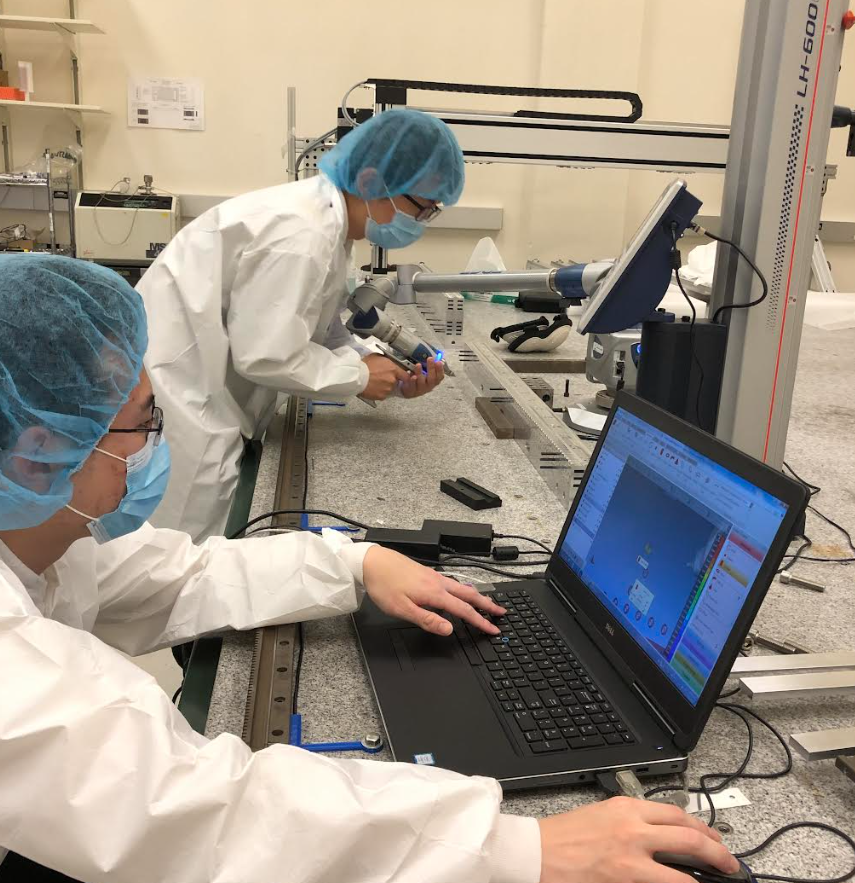
\includegraphics[width=0.415\linewidth]{figures/ch7-sMDT/measure-combs.PNG}}
 \subfloat[]{
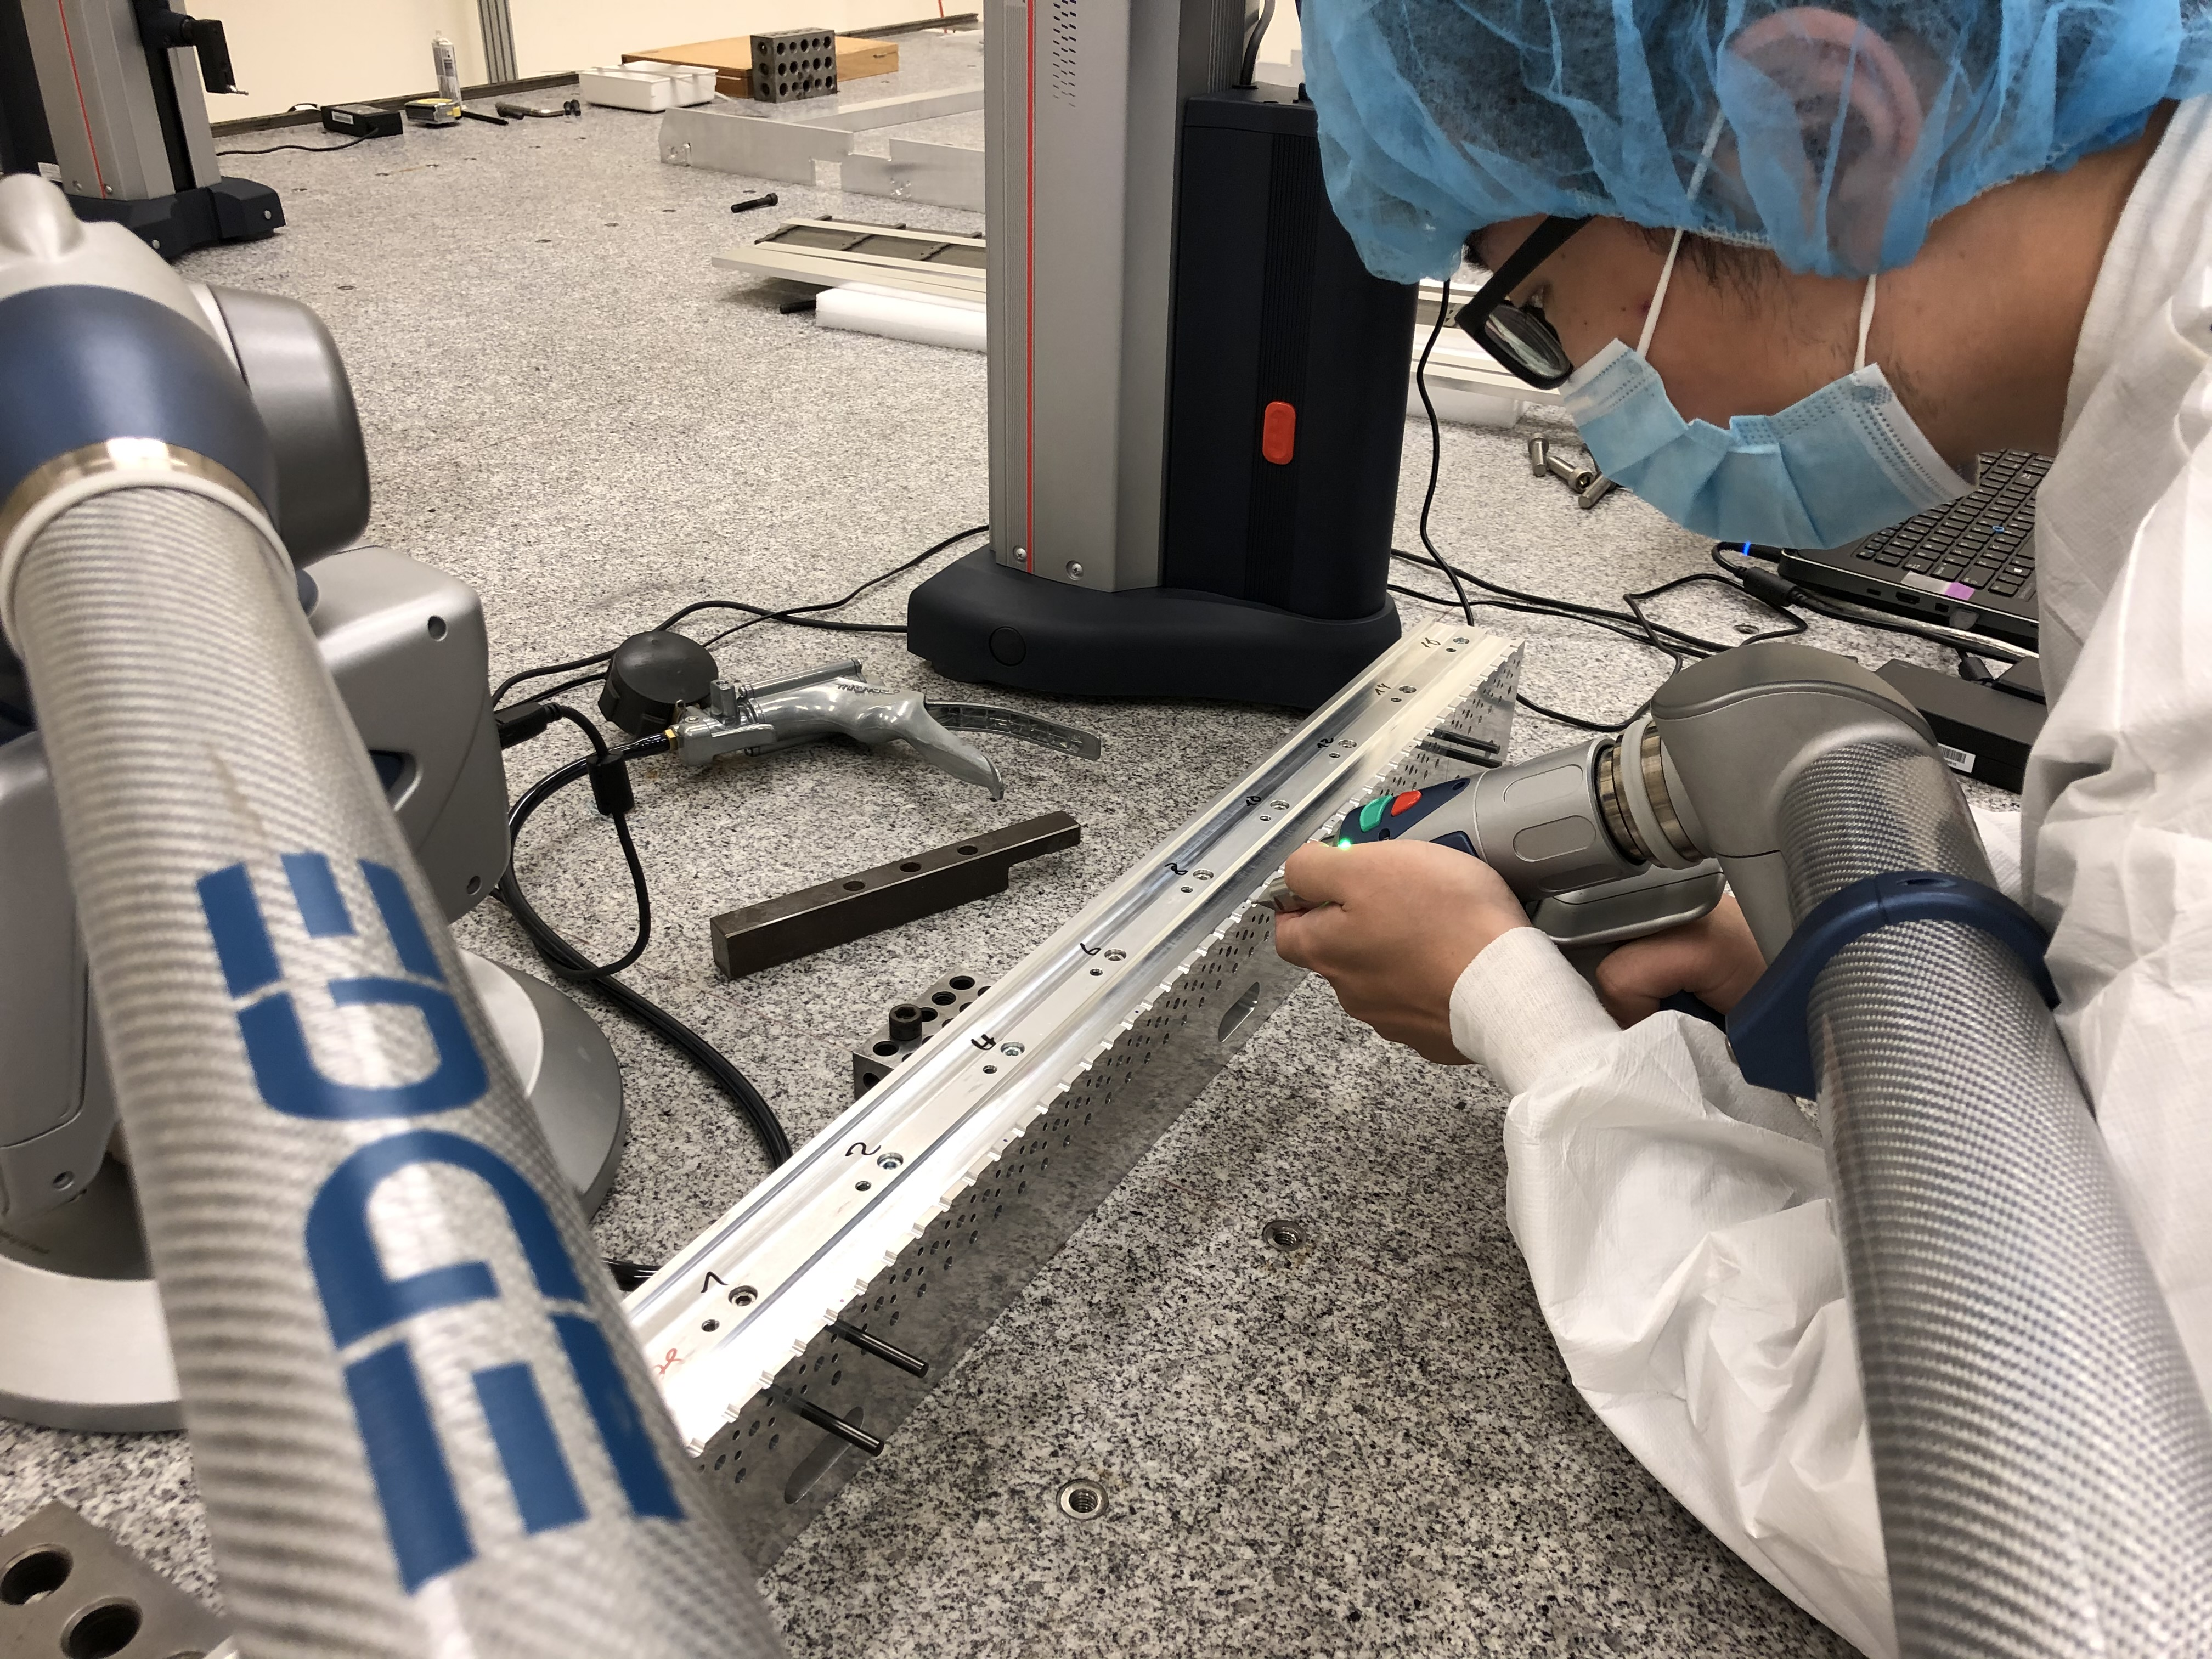
\includegraphics[width=0.57\linewidth]{figures/ch7-sMDT/measure-jigging.jpeg}}
    \caption{Measuring the precision combs using the computing-aid FORA-arm. (a) set up the measurement coordinates, and (b) measure the comb pitch by the author.}
    \label{fig:sMDT-base-plates}
\end{figure}

Figure~\ref{fig:sMDT-base-plates} shows the comb measurements performed using a coordinate-measuring FORA arm, which determines three-dimensional points with a precision better than 10~$\mu$m after calibration. The measured wire-pitch distributions for both comb sets are shown in Figure~\ref{fig:sMDT-wirepitch}. The mean wire pitch agrees with the design value, with an RMS of about 4~$\mu$m.
\begin{figure}[!htb]
    \centering
    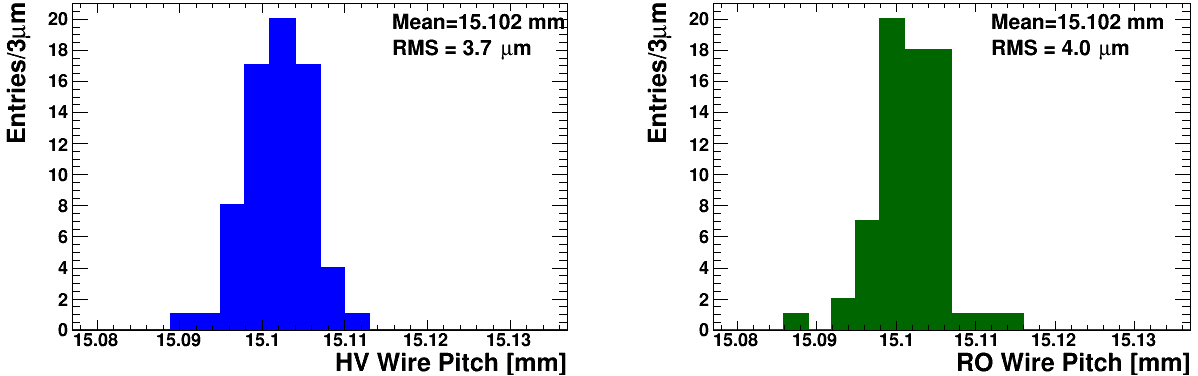
\includegraphics[width=0.90\linewidth]{figures/ch7-sMDT/WirePitch.png}
    \caption{Measurements of the wire pitch for readout and high-voltage side combs. }
    \label{fig:sMDT-wirepitch}
\end{figure}

During chamber assembly, the precision cylinder of each tube end-plug is placed in the open half-cylinders of the end-combs. The lower comb constrains the horizontal position of the tube, while the upper comb is screwed onto the lower comb to fix the vertical position.

The tubes are kept straight by resting on four base inner-combs mounted on the granite table. When gluing the fifth tube layer onto the spacer frame bars, an additional set of four secondary inner-combs is placed on top of the bottom multilayer to guide the tube positioning. These combs serve the same purpose as the base inner-combs when assembling the top multilayer.

To control tube straightness and prevent bowing during gluing, four upper comb weights with 7.5 mm radius semicircular grooves are placed on top of each newly glued tube layer.

%%%%%%%%%%%%%%%%
\noindent{\bf 2) Automatic glue machine} \\
A large gantry-mounted, computer-controlled glue-dispensing system (see Figure~\ref{fig:sMDT-chamber-granite}) was designed and built at the University of Michigan. The system controls the three-dimensional motion of the dispensing tip and the piston drive of the epoxy cartridge. The gantry is constructed from $\mathrm{7.6~cm \times 15.2~cm}$ aluminum extrusions mounted on rail carriages that move directly on the granite table surface.

The two rails are aligned to be parallel within 7~$\mu$rad. Motion along the $X$ direction is driven by a toothed rail on one side of the granite table, allowing the gantry to travel along the table length with a precision of 0.1~mm. The linear rails and carriages are regularly cleaned and lubricated to minimize friction.

The $Y$, $Z$, and $A$ axes are driven by linear actuators. The $Y$ axis, with a range of 2.5~m, moves along the tube direction, while the $Z$ axis provides 0.5~m of vertical travel to position the glue cartridge from the first tube layer to the top support structures of a chamber. The $A$ drive controls epoxy dispensing and operates in steps of 0.26~mm, corresponding to approximately 0.5~cc of epoxy per step.

The control software is implemented in \textsc{LabVIEW}, interfacing with the motor drivers supplied by the manufacturers. Predefined motion sequences and dispensing patterns are developed and tested to optimize the gluing of tube layers, spacer frames, and support structures.

%%%%%%%%%%%%%%%%%
\subsection{Precision comb base-plates set up and measurements}

The base end- and middle-combs and two base plates must be precisely positioned on the granite table to ensure the chamber can be built precisely based on the design geometry. Their setup was performed iteratively, alternating between mechanical adjustments and precision measurements. Positions were measured using a FARO-arm for three-dimensional coordinates with a precision better than 10~$\mu$m, and a height gauge with a precision of 5~$\mu$m relative to the granite surface.
\begin{figure}[!htb]
    \centering
    \subfloat[]{
 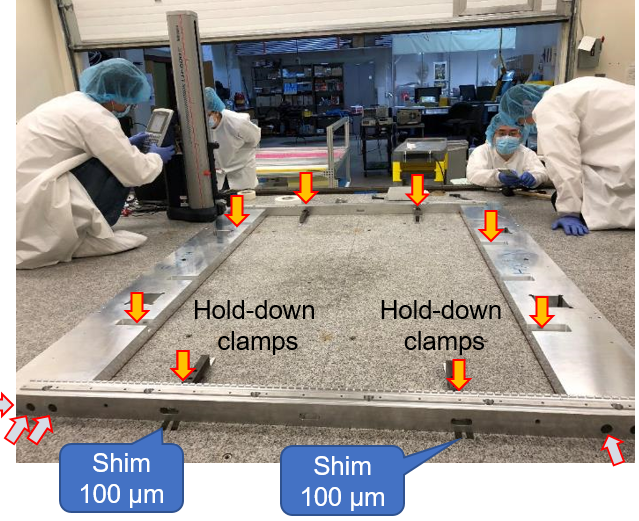
\includegraphics[width=0.6\linewidth]{figures/ch7-sMDT/base-plates.PNG}}
 \subfloat[]{
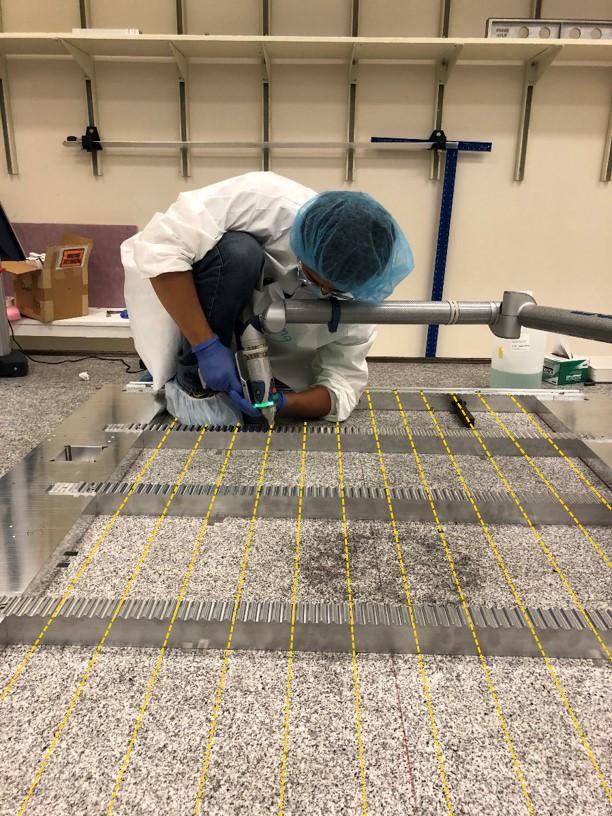
\includegraphics[width=0.37\linewidth]{figures/ch7-sMDT/middle-comb.png}}
    \caption{Set up of base combs: 
    (a) The two precision base end-combs are    
        connected to two sidebars by bolts indicated by the white/red arrows.
        The yellow/red arrows point to the 
        hold-down clamps of the base jigging;
    (b) The inner base-combs are connected 
        to the two sidebars. }
    \label{fig:sMDT-base-plates}
\end{figure}

The two precision end-combs are bolted to cross-plates at opposite ends of the two heavy cross-plates. They are also clamped on the granite table. Precision shims are used to adjust the heights of the base combs and plates, as shown by the red arrows in Figure~\ref{fig:sMDT-base-plates}(a). The combs are aligned parallel to each other and perpendicular to the wire direction, which is itself aligned with the glue machine $Y$ axis. 
%This alignment is periodically verified and adjusted if necessary.
%
The inner base combs, shown in Figure~\ref{fig:sMDT-base-plates}(b), are also connected to the cross-plates and ensure tube straightness during gluing. They are aligned along the tube direction (yellow dashed lines in Figure~\ref{fig:sMDT-base-plates}(b)) and in height to better than 50~$\mu$m, measured with the FARO-arm.
 
The squareness of the base-comb assembly was checked with the FARO arm by measuring the diagonals defined by precision half-cylinders placed in comb notches 4 and 67. The two diagonals differ by 15~$\mu$m, and the angle between the comb assembly and the long base plates deviates by at most $0.0018^\circ$ ($0.03$~mrad) from $90^\circ$, as shown in Figure~\ref{fig:sMDT-base-measurement}.
\begin{figure}[!htb]
    \centering
    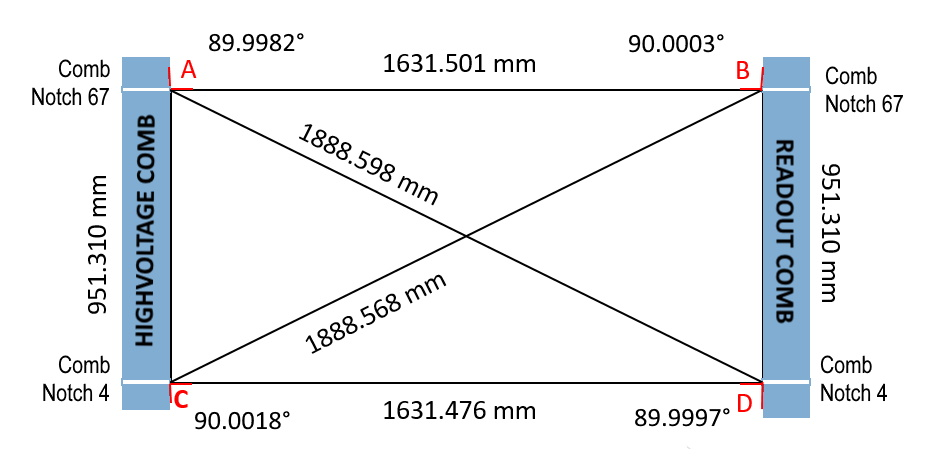
\includegraphics[width=0.75\linewidth]{figures/ch7-sMDT/BaseComb-setup.jpg}
    \caption{Base comb layout geometry and measured distances and angles. }
    \label{fig:sMDT-base-measurement}
\end{figure}

Both base combs exhibited a bowed shape after the initial setup on the granite table, as shown by the green points in Figure~\ref{fig:base-tuning}. The same deformation was observed in subsequent layers added to the base comb.
\begin{figure}[!htb]
    \centering
    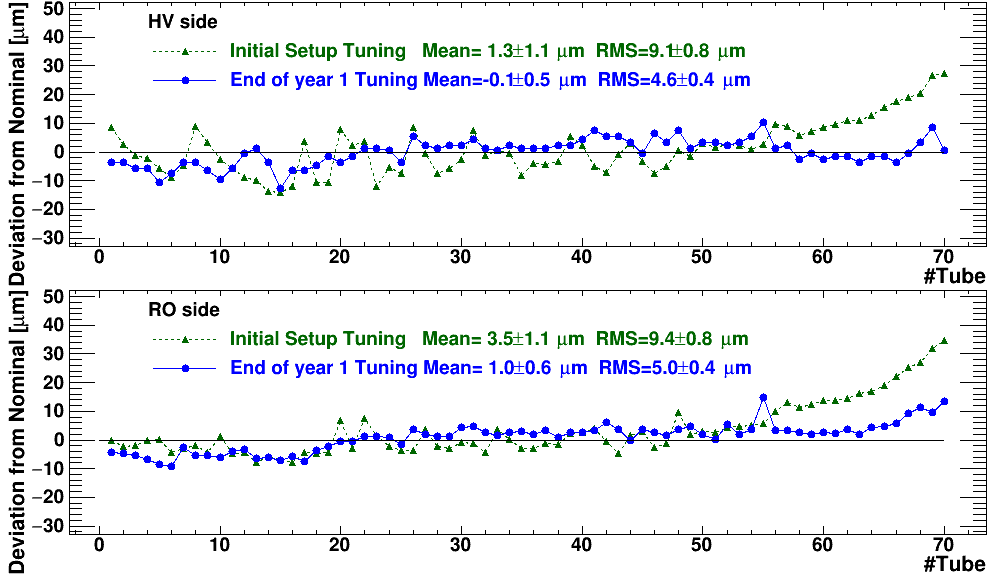
\includegraphics[width=0.8\textwidth]{figures/ch7-sMDT/JiggingTuning.png}
    \caption{Base end-comb cylinder center height measurements relative to the target wire height above the granite surface for the HV and RO sides, showing the initial setup and the retuned configuration.}
    \label{fig:base-tuning}
\end{figure}

The combs were flattened through an iterative procedure: loosening the screws that fix the comb ends to the side cross-plates, applying downward pressure to the outer ends, and re-tightening the screws while monitoring the height measurements in real time. This process was repeated until sufficient flatness was achieved. The tuned comb shapes are shown by the glue points in Figure~\ref{fig:base-tuning} for comparison.
The final standard deviation (RMS) of the comb flatness is below 10~$\mu$m for both base combs.

%%%%%%%%%%%%%%%%%%%%%%%%%%%%%%%%%%%%%%%%%%%

\subsection{Chamber assembly} \label{chap:cham-assembly}

An sMDT chamber is assembled on the granite table by gluing eight tube layers together with a spacer frame that contains the optical in-plane alignment system, using the precision jigging setup. The assembly sequence takes about five days: two days to glue the bottom multilayer, one day to glue the spacer frame and the first layer of the second multilayer, and two additional days to glue the remaining three tube layers of the top multilayer.
\begin{figure}[!htbp]
    \centering
    \subfloat[]{
        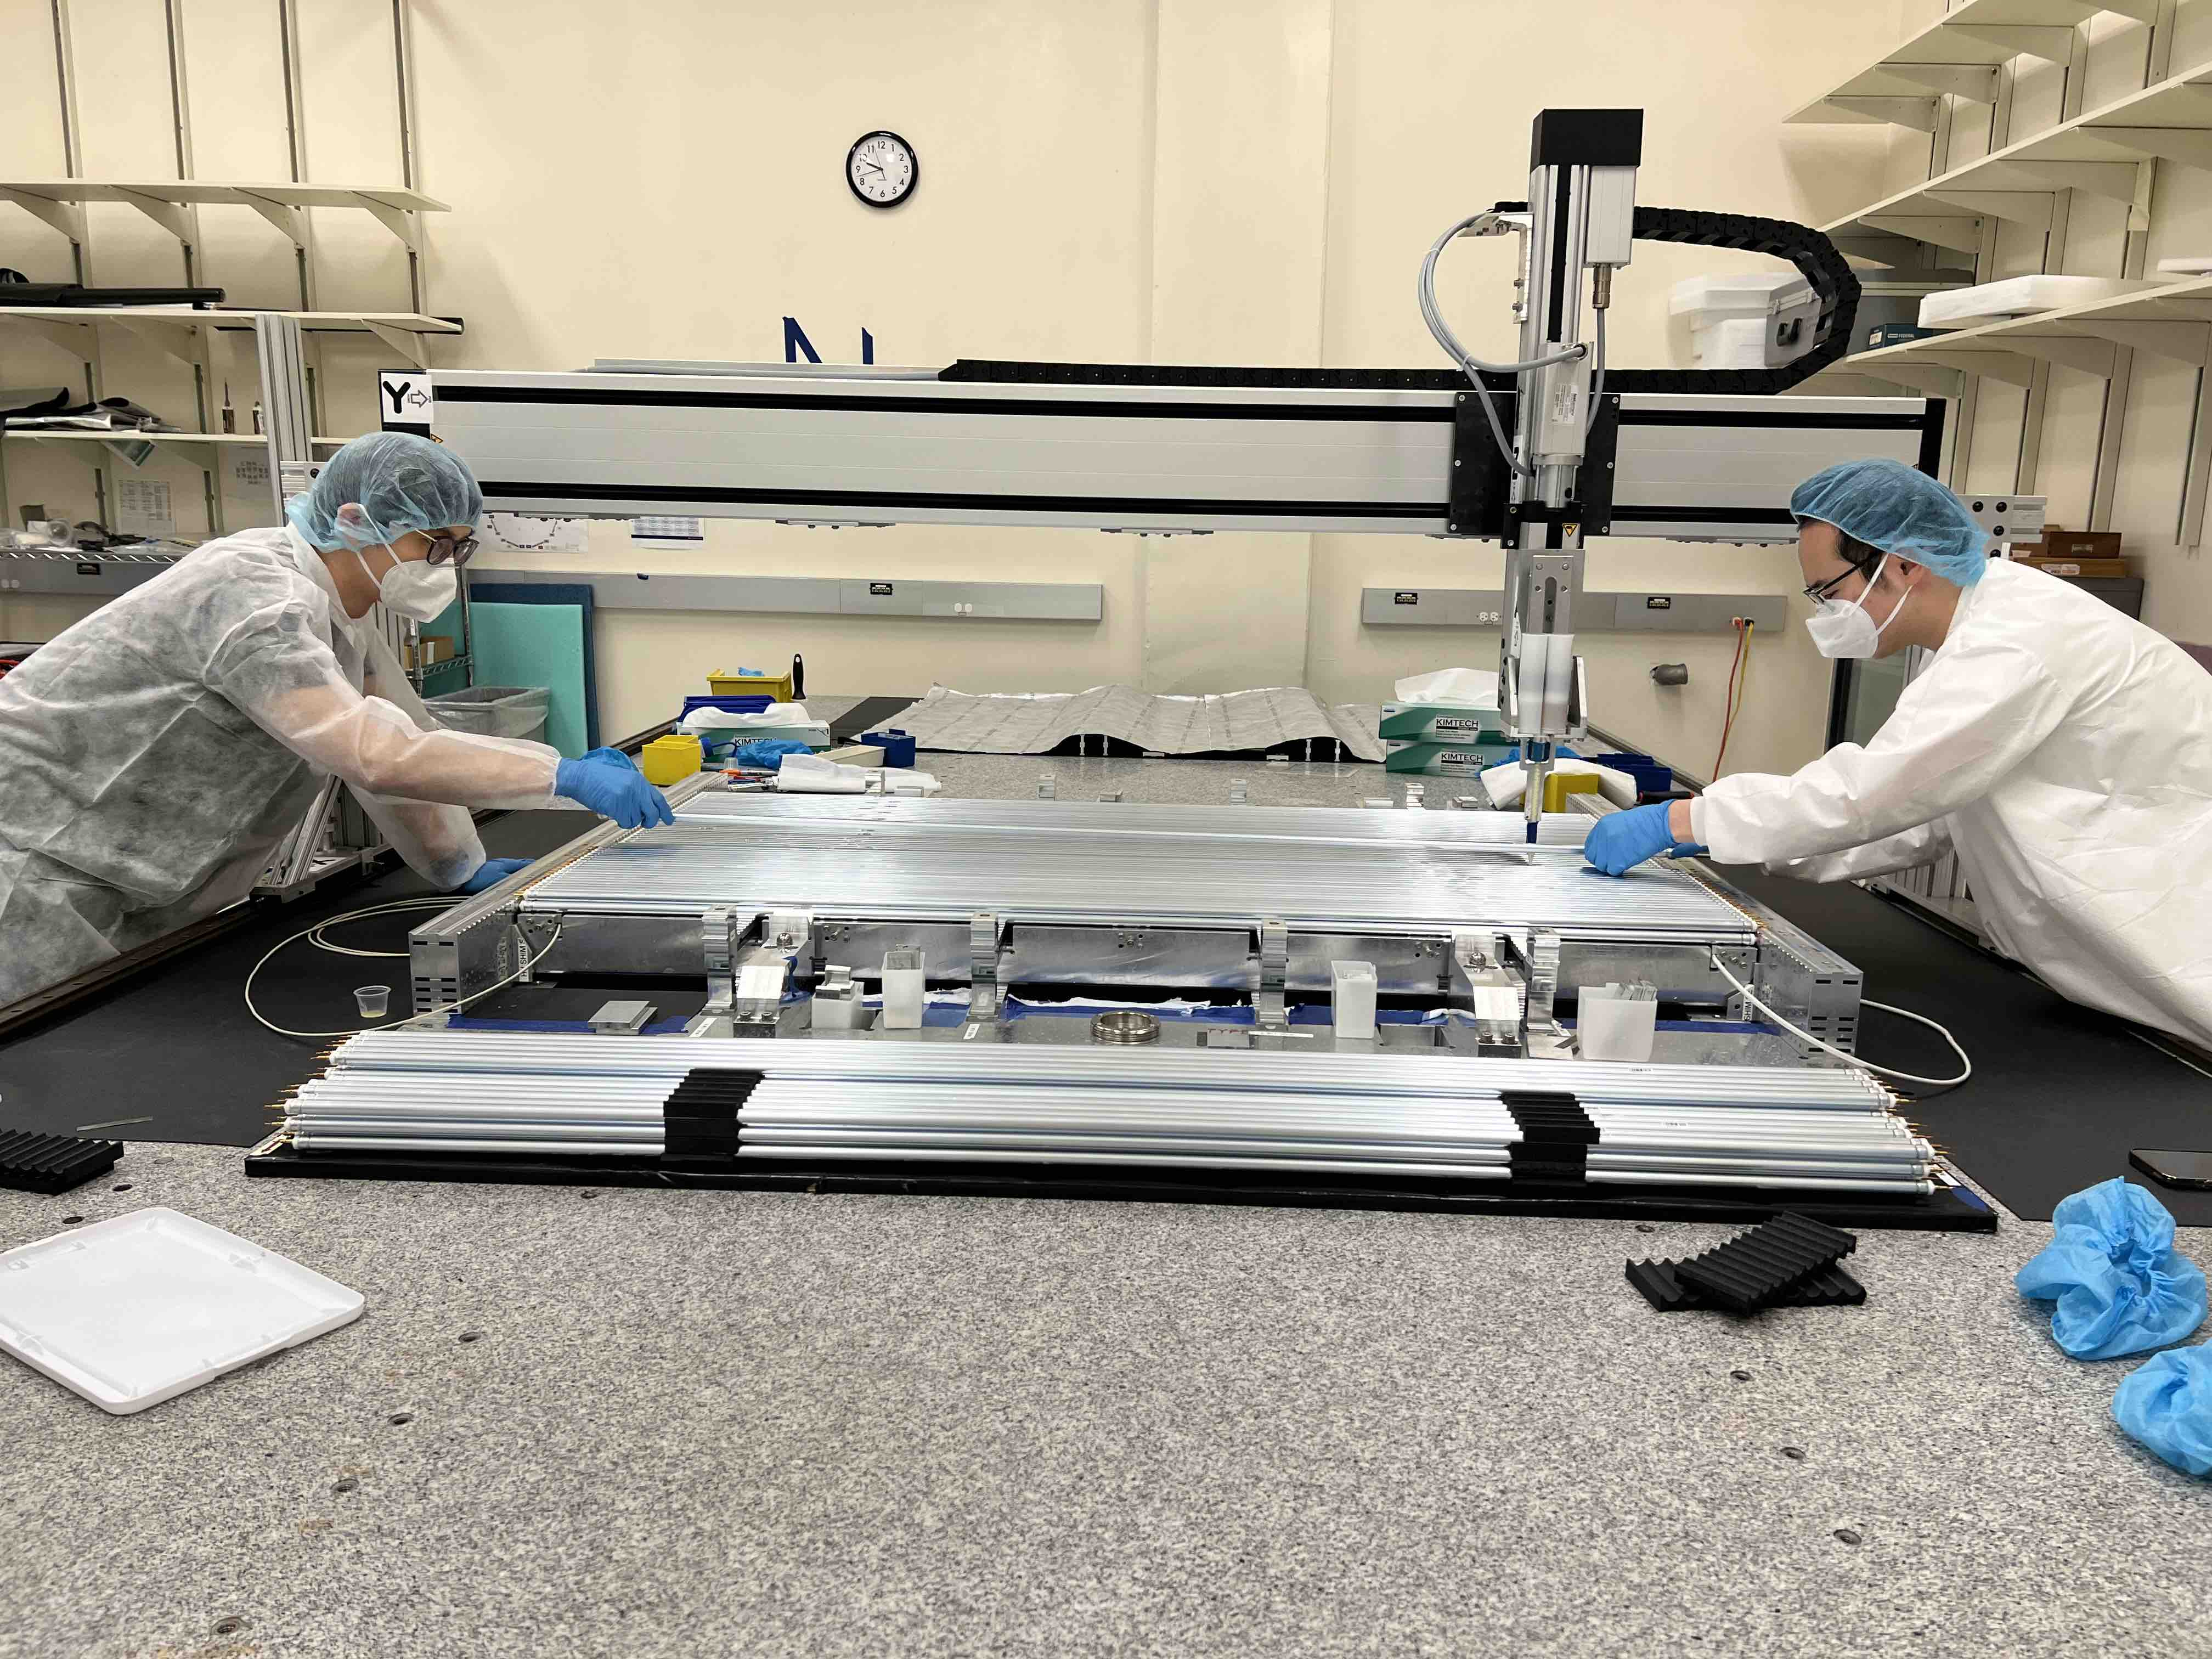
\includegraphics[width=0.62\linewidth]{figures/ch7-sMDT/glue-tube.jpg}}
    \subfloat[]{
        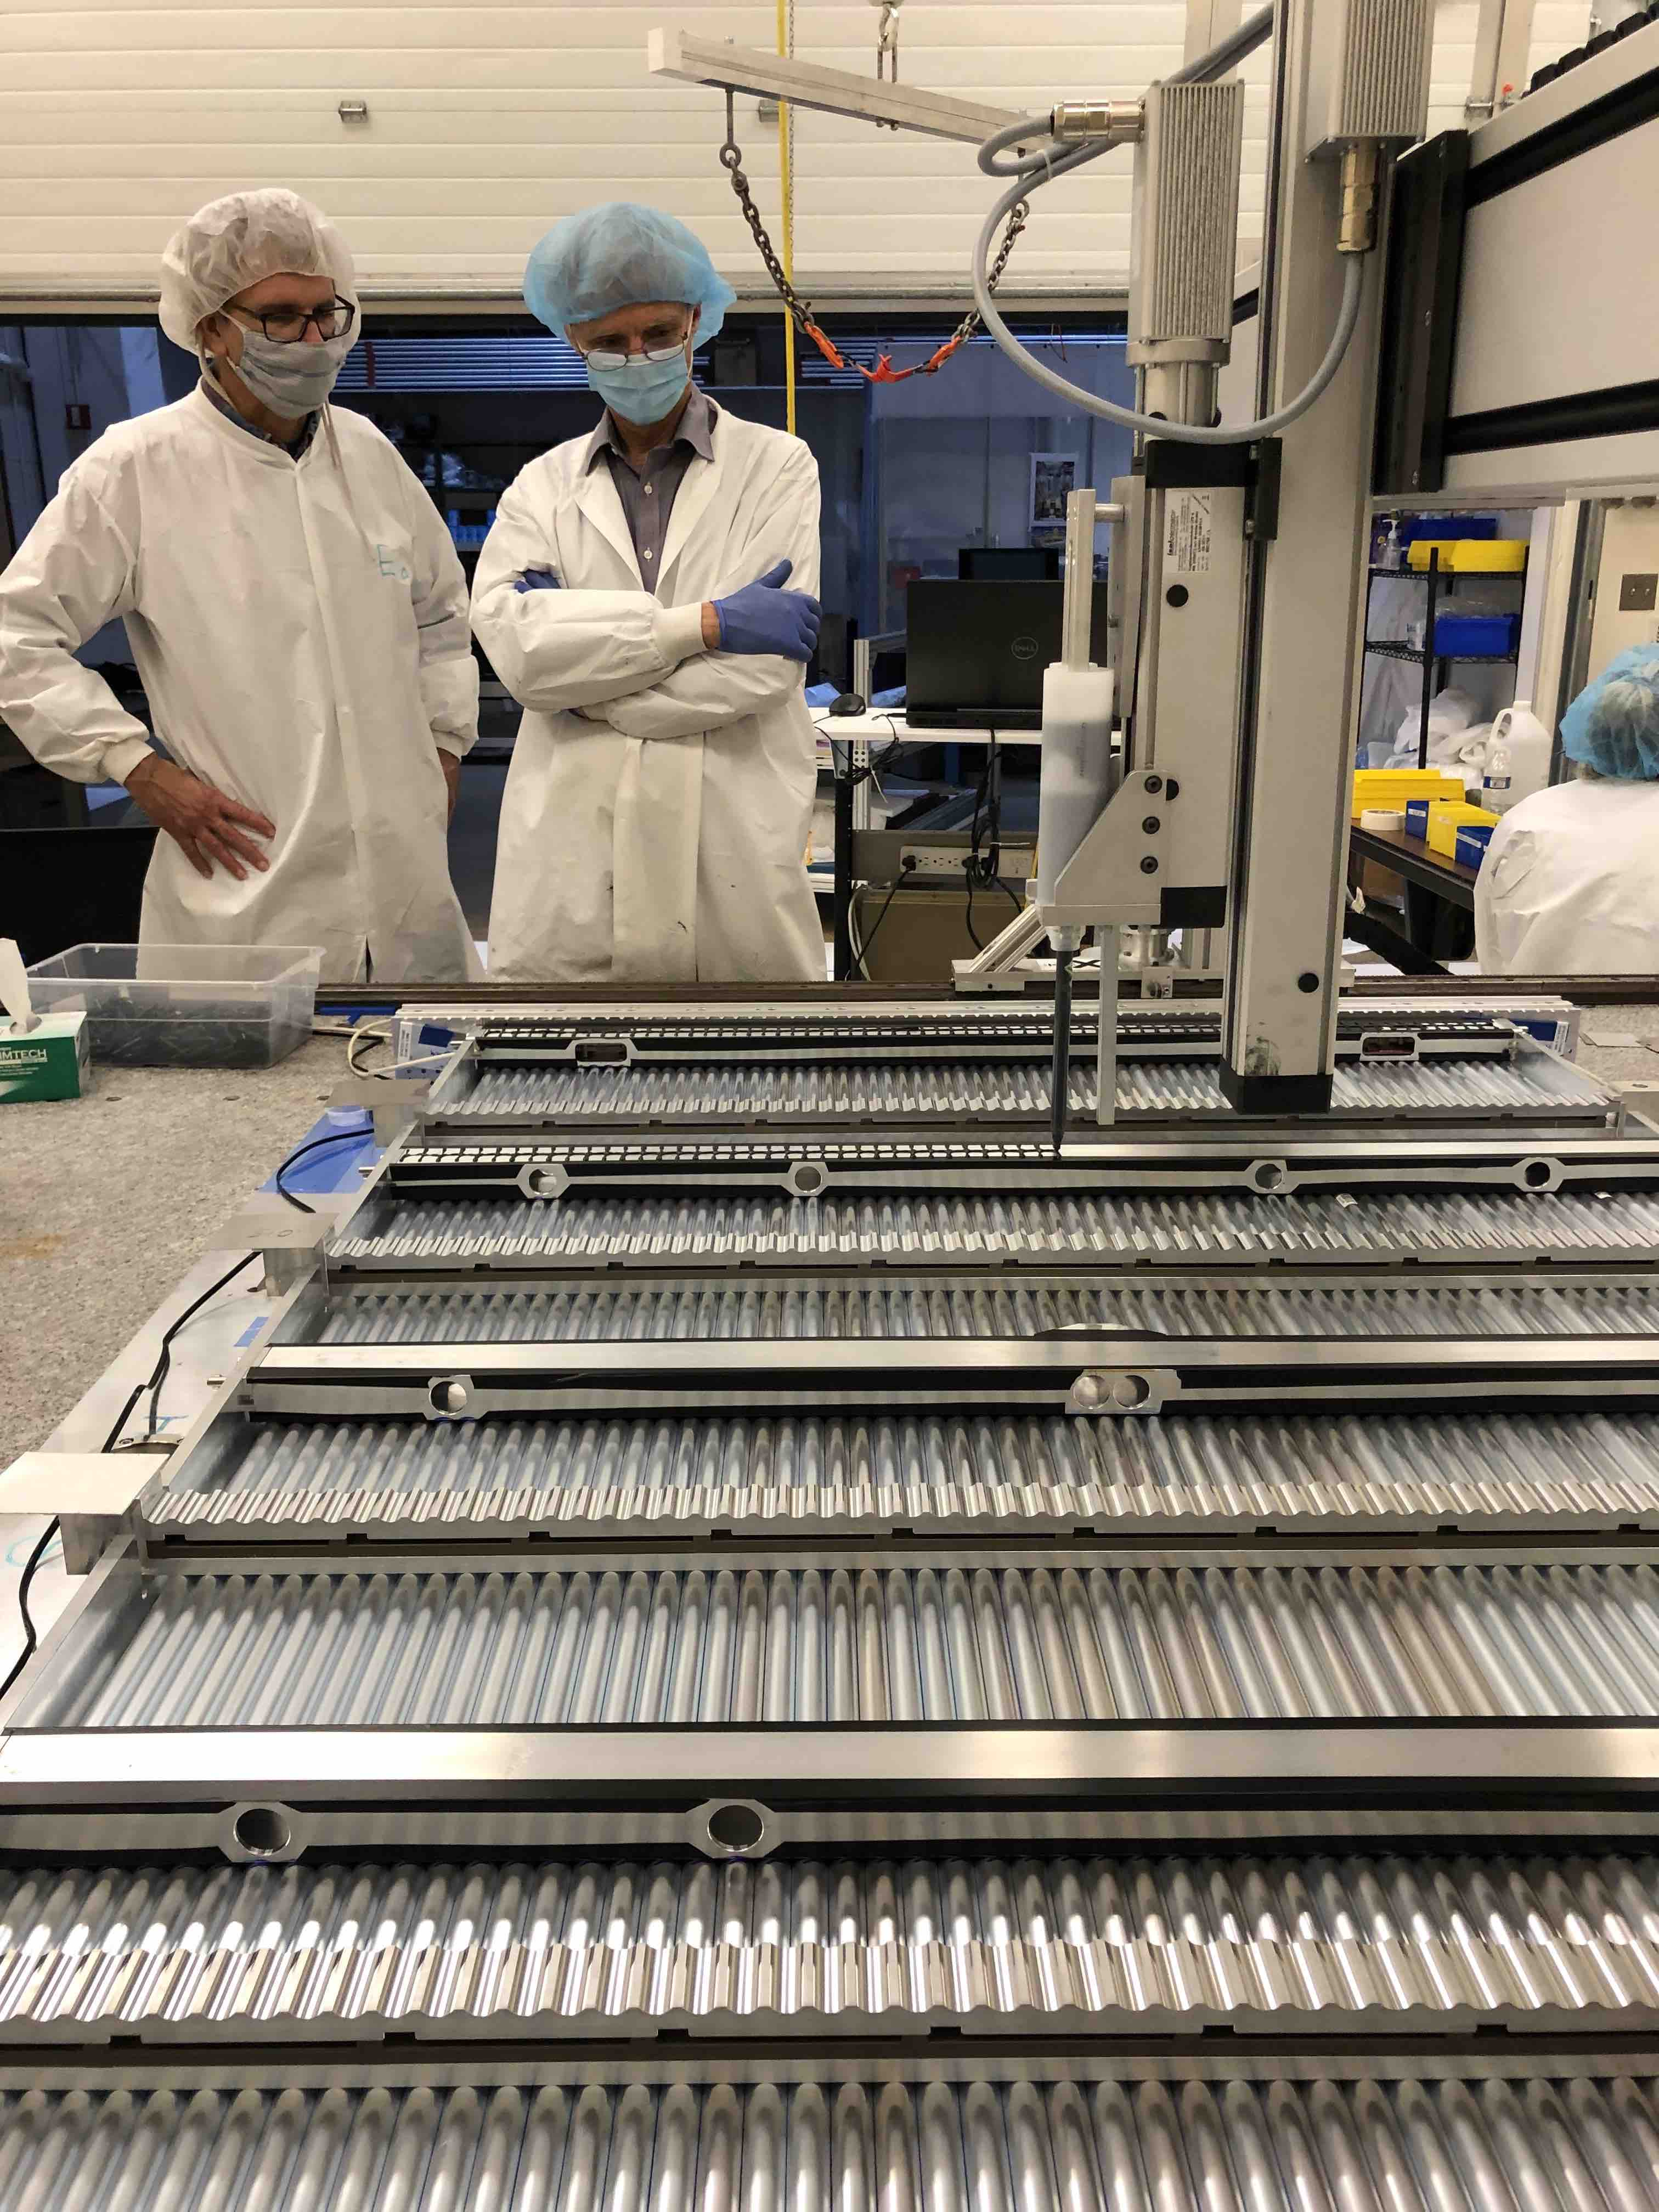
\includegraphics[width=0.35\linewidth]{figures/ch7-sMDT/glue-Spacer.jpg}}
    \caption{(a) Two operators placing a tube on the combs after automatic glue application on the lower tube layer. (b) Gluing the pre-assembled spacer frame on top of the bottom multilayer of the chamber.}
    \label{fig:glue-chamber}
\end{figure}
\begin{figure}[!htbp]
    \centering
        \subfloat[]{
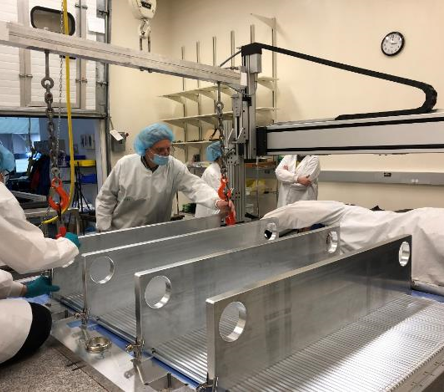
\includegraphics[width=0.45\linewidth]{figures/ch7-sMDT/put-weights.PNG}}
    \subfloat[]{
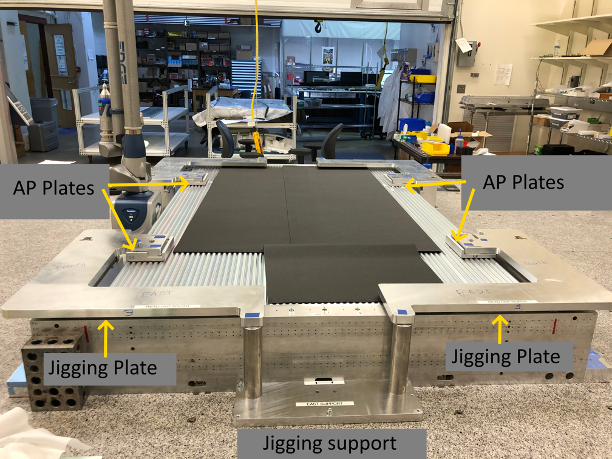
\includegraphics[width=0.53\linewidth]{figures/ch7-sMDT/CCC-jigging-plates.PNG}}
\caption{(a) Put weights on top of the glued tube layer. (b) Glue the AP-plates on the top of the chamber. }
    \label{fig:sMDT-weight}
\end{figure}

Tube-layer gluing is performed by two operators (Figure~\ref{fig:glue-chamber}(a)), who place the tubes on precision combs with all endplug plastic insulators touching the RO-side end comb. This ensures proper tube alignment for later installation of the readout electronics. An automatic glue machine dispenses Araldite~2011 glue dots at 11 equidistant positions in each groove between the tubes. The tubes of the next layer are then placed into the wet glue and held in position by the end combs and upper comb weights.

%After a tube layer is placed in the wet glue with the end plugs resting in the half-notches of the lower end combs, the next level of end combs is installed on top and clamped on both sides with a torque of 7.5~Nm per screw.
%
While the glue is still wet, four comb weights are placed on the top tube layer, as shown in Figure~\ref{fig:sMDT-weight}(a). Each weight has a bottom surface machined with a half-cylinder profile matching the tube layer and is supported by precision riser blocks that define its height and lateral position. These weights keep the top layer straight during curing and prevent the outermost tubes from bowing outward. After overnight curing, the weights are removed, and the tube glue process continues. 
%and ground screws, preloaded on comb layers 2, 3, 4, 6, 7, and 8 (counting from the bottom), are inserted into the gaps between the tubes.

\begin{figure}[!htbp]
    \centering
        \subfloat[]{
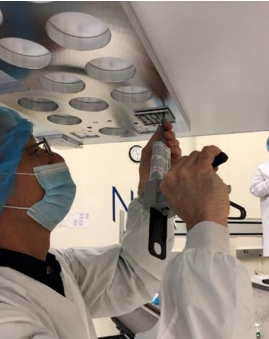
\includegraphics[width=0.325\linewidth]{figures/ch7-sMDT/glue-CCC.PNG}}
    \subfloat[]{
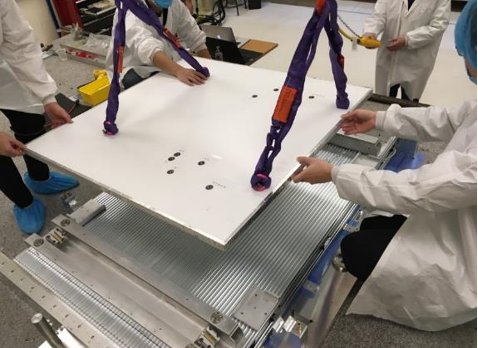
\includegraphics[width=0.56\linewidth]{figures/ch7-sMDT/Glue-big-plate.PNG}}
\caption{(a) Glue is applied to the CCC platforms, which are mounted on the large jig plate. (b) Installation of the CCC platforms in the chamber. After the platforms are glued to the chamber, they are detached from the jig plate before the jig plate is removed.}
    \label{fig:sMDT-CCC-installation}
\end{figure}

%%%%%%%%%%%%%%%%%%%%%%%%%%%%%%%%%%
After the base chamber is glued, platforms for mounting the Axial--Praxial (AP) sensors and the Chamber-to-Chamber Connection (CCC) alignment sensors are attached to the chamber top surface. Additional platforms for magnetic-field sensors are also installed.
%
The positions of these platforms relative to the wire grid, with heights referenced to the granite table, must be accurate within 0.20~mm and known to better than 0.03~mm. This precision is achieved using two dedicated jigging sets that predefine the platform locations relative to the perpendicular distance from the first wire of the chamber.
%
Figure~\ref{fig:sMDT-weight}(b) shows the jig used to glue the AP plates, while Figure~\ref{fig:sMDT-CCC-installation} illustrates the glue application for the CCC platforms in the large-plate jig and their installation on the chamber in panels (a) and (b).

%%%%%%%%%%%%%%%%%%%%%%%%%%%%%%%%%%
\subsection{Precision measurement of the platform and tube positions}
\label{faromeasurement}

Precise measurement of the platform and tube positions is a critical step in chamber construction to ensure the positional accuracy of the platforms and wires required for precise muon tracking. The measurements are performed on a granite table using a computer-aided FARO-arm and a height-gauge. Typically, two operators require about five days to complete the full set of measurements.

The platform positions are first measured with the FARO-arm, as shown in Figure~\ref{fig:measure-platform}(a), using computer-defined coordinates $(x, y, z)$ referenced to the first wire, the granite table surface, and the outer surface of the end-comb.

\begin{figure}[!htbp]
    \centering
    \subfloat[]{
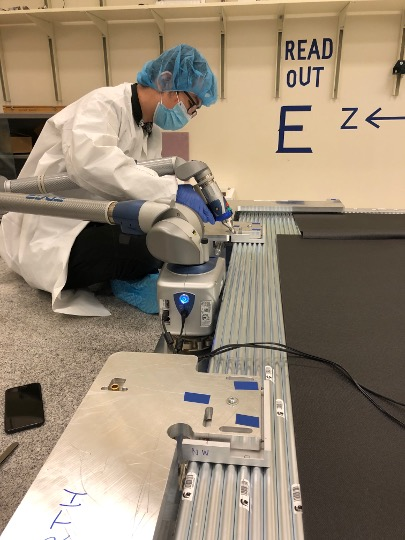
\includegraphics[width=0.23\linewidth]{figures/ch7-sMDT/Chuanshun-meaure-cccplate.jpg}}
    \subfloat[]{
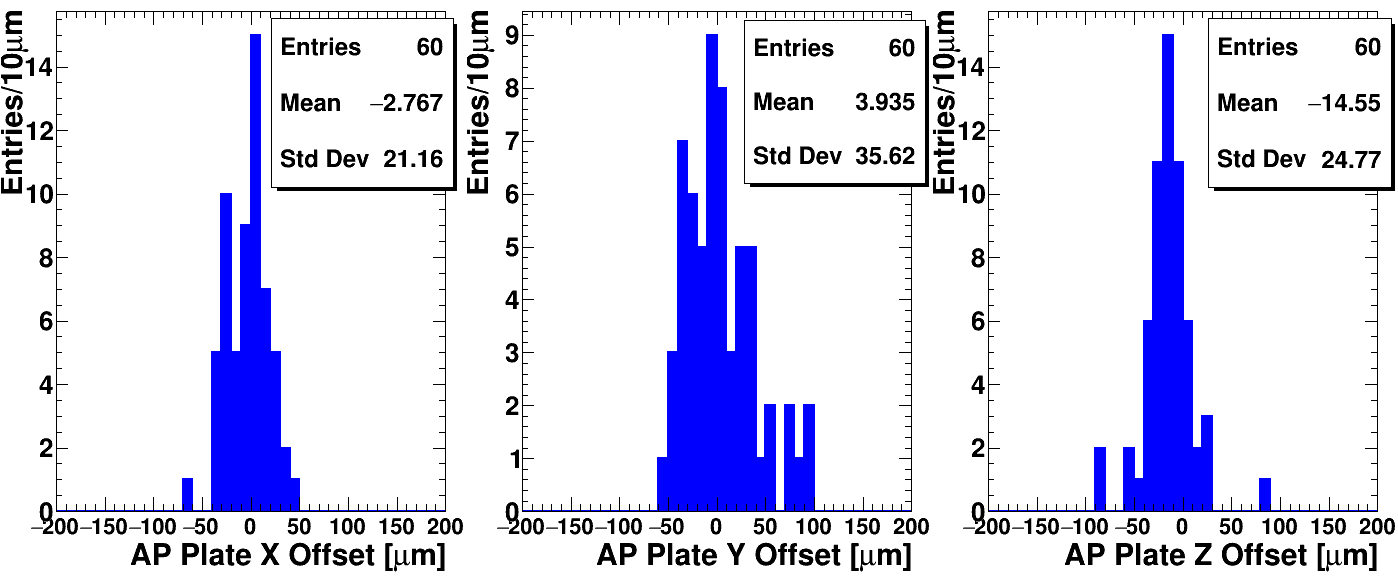
\includegraphics[width=0.76\textwidth]{figures/ch7-sMDT/APplate_XYZ1D_ROHV_30sMDT.png}}
\caption{(a) Measurement of the platform position using the FARO arm by the author. (b) Distributions of the measured AP-platform position offsets in $X$, $Y$, and $Z$ from the nominal values.}
    \label{fig:measure-platform}
\end{figure}

Several distances corresponding to reference points are measured on the three mutually perpendicular surfaces of each AP and B-field platform to determine their three-dimensional positions relative to the reference coordinates. Each distance measured with the FARO-arm is compared with its nominal value, and the deviation from the target value is calculated.

Figure~\ref{fig:measure-platform}(b) shows the measured AP-platform position offsets in $x$, $y$, and $z$ with respect to the nominal values. All AP platforms are positioned well within the required maximum deviation of 200~$\mu$m from the nominal position. Similar results are obtained for the CCC and B-field sensor platforms.

\begin{figure}[!htbp]
    \centering
    \subfloat[]{
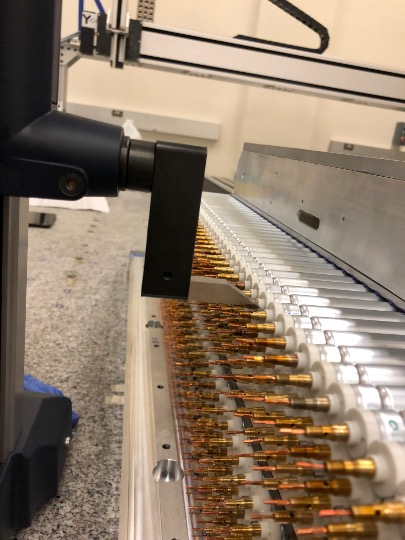
\includegraphics[width=0.28\linewidth]{figures/ch7-sMDT/measure-tube-height.JPG}} \hspace{0.4cm}
    \subfloat[]{
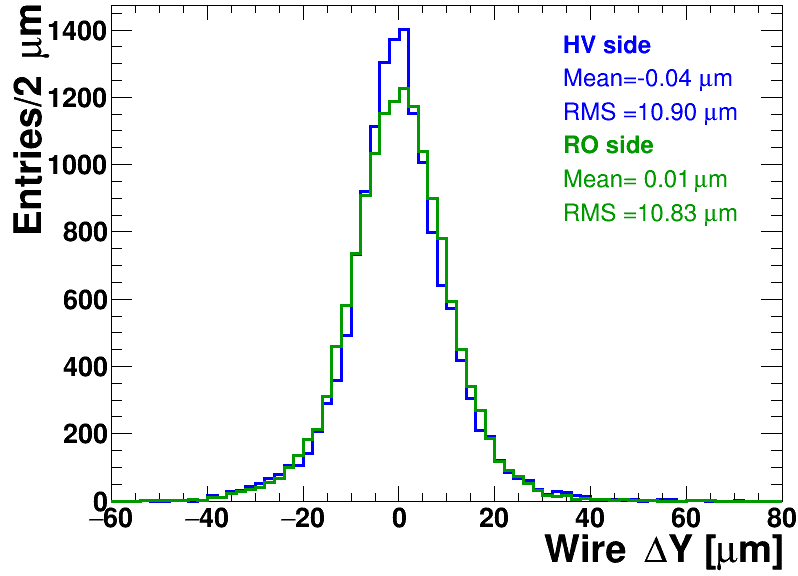
\includegraphics[width=0.53\linewidth]{figures/ch7-sMDT/ChamberWireOffset_30sMDT.png}}
\caption{(a) Measurement of the tube height relative to the granite table surface using a precision height gauge. (b) Distributions of the measured tube height offsets from the nominal values at the two ends of the tubes.}
    \label{fig:tube-position}
\end{figure}

The tube height relative to the granite table surface is measured using the precision end-plug cylinder surfaces with a height-gauge equipped with a flat probe, as shown in Figure~\ref{fig:tube-position}(a). 

The histograms in Figure~\ref{fig:tube-position}(b) show the deviations of the measured tube heights from the nominal values for each tube layer at both tube ends. The RMS of these distributions is below 11~$\mu$m, which is well below the 20~$\mu$m requirement, indicating that the tubes are glued into the chamber with high precision.

%%%%%%%%%%%%%%%%%%%%%%%%%%%%%%%%%%%%%%%%%%%%%%%%%%%%%
\subsection{Chamber service installation and test}
The assembly combs are removed, and the chamber is lifted from the granite table (see Figure~\ref{fig:lift-chamber}) and transferred to the chamber rotation cart for service installation.
\begin{figure}[!htbp]
    \centering
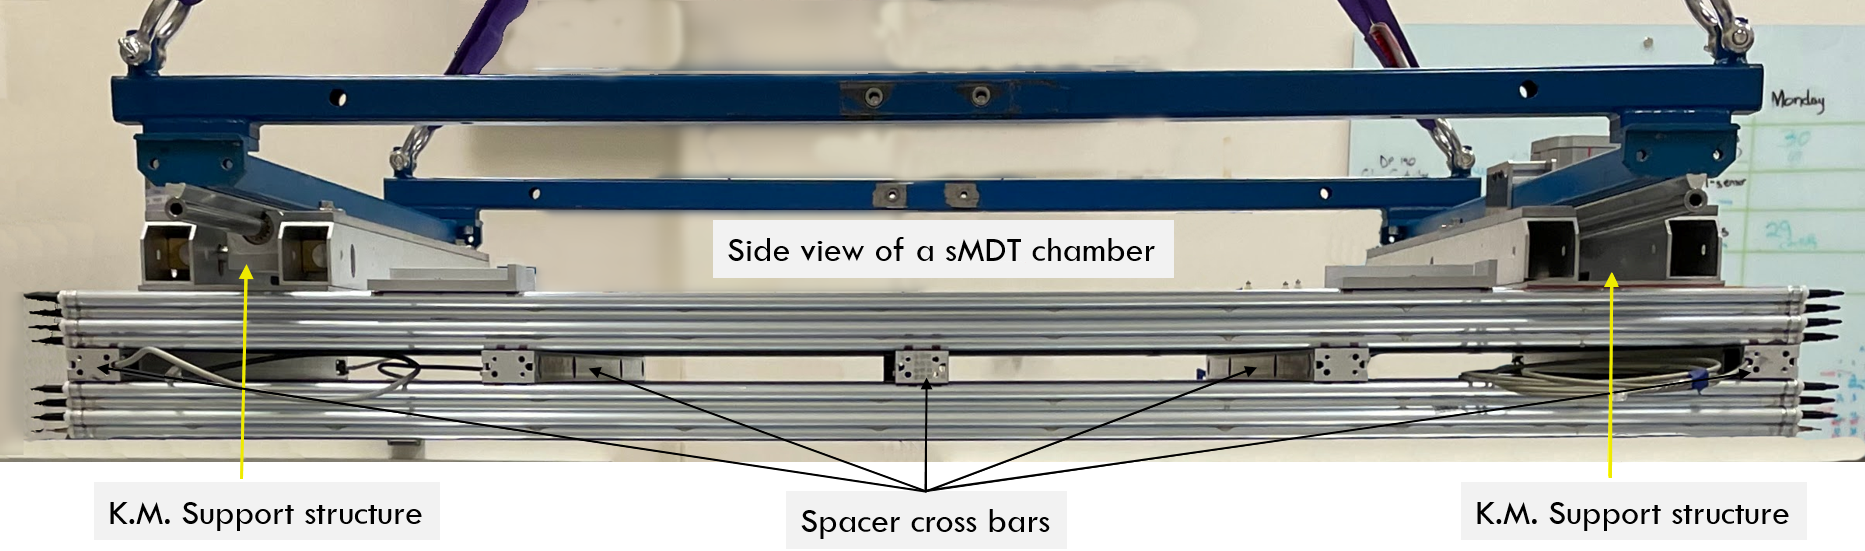
\includegraphics[width=0.90\linewidth]{figures/ch7-sMDT/Chamber-sideview.PNG}
\caption{An assembled chamber lifted by an overhead crane above the granite table.} 
    \label{fig:lift-chamber}
\end{figure}

The chamber services are installed while the chamber is mounted on the rotation cart, shown in Figure~\ref{fig:sMDT-rotation-cart}(a). These services include temperature sensors and cables, grounding foil, gas manifolds, hedgehog electronics cards, Faraday cages, and ground straps.
\begin{figure}[!htbp]
    \centering
        \subfloat[]{
   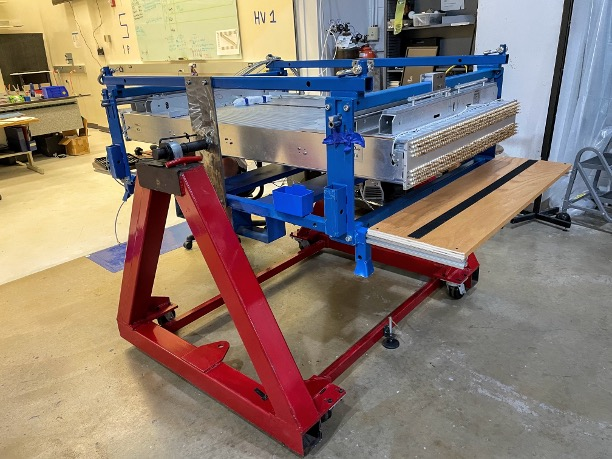
\includegraphics[width=0.39\linewidth]{figures/ch7-sMDT/rotation-cart-2.jpg}}
        \subfloat[]{
    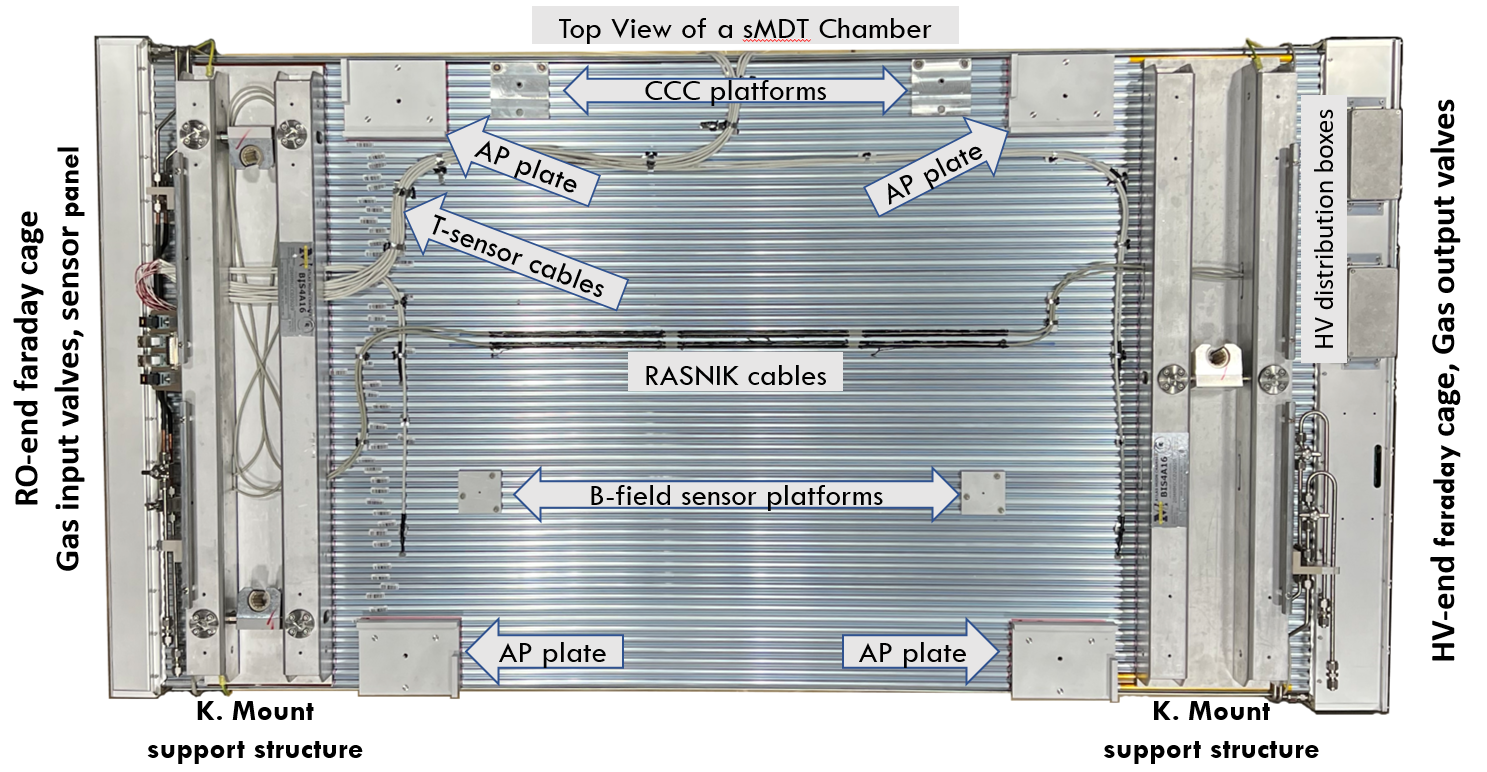
\includegraphics[width=0.6\linewidth]{figures/ch7-sMDT/Chamber-topview.PNG} }
\caption{(a) Chamber mounted on a rotation cart. (b) Top view of a chamber with services installed. }
    \label{fig:sMDT-rotation-cart}
\end{figure}

Twelve temperature sensors with readout cables are glued to the chamber surface: six on the bottom surface and six on the top tube layer. 
Thermal contact between the sensors and tubes is ensured using thermal epoxy paste. 
All sensor cables are routed to the chamber top surface through a hole in the RO-side support structure (Figure~\ref{fig:sMDT-rotation-cart} (b)). 
Cables for the in-plane alignment system control and readout are also routed along the top surface and connected to a readout panel mounted on the RO-side support structure.

A perforated foil is wrapped around each end of the chamber to provide a common ground connection from the tube walls to the RO and HV hedgehog cards. 
This foil forms the internal wall of the Faraday cage enclosing the electronics. 
Grounding pins are screwed into the grounding anchors installed during gluing and tightened against the foil. 
These pins are installed after the gas system and before the hedgehog cards are mounted.

\begin{figure}[!htbp]
    \centering
    \subfloat[]{
    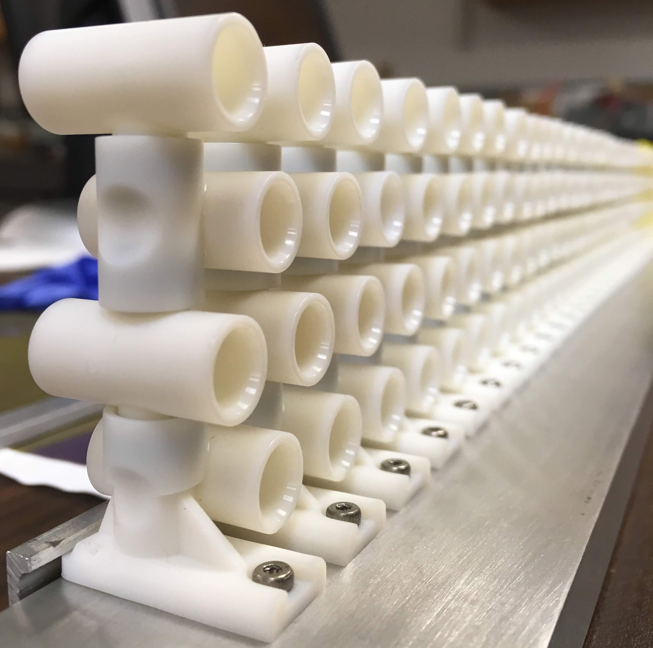
\includegraphics[width=0.28\linewidth]{figures/ch7-sMDT/gas-bar.PNG} }
        \subfloat[]{
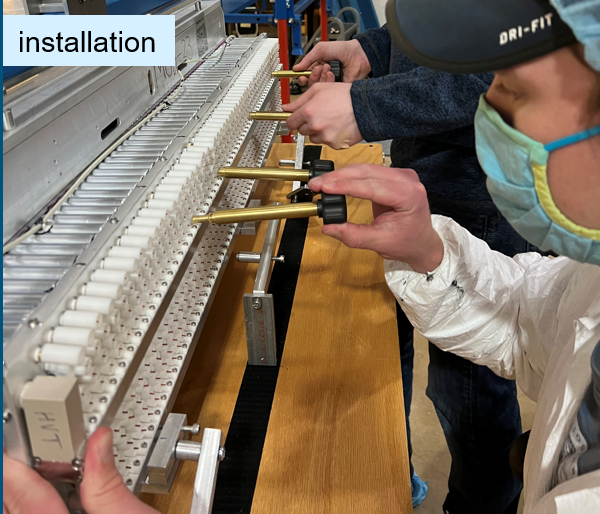
\includegraphics[width=0.325\linewidth]{figures/ch7-sMDT/gas-bar-installation.PNG}}
        \subfloat[]{
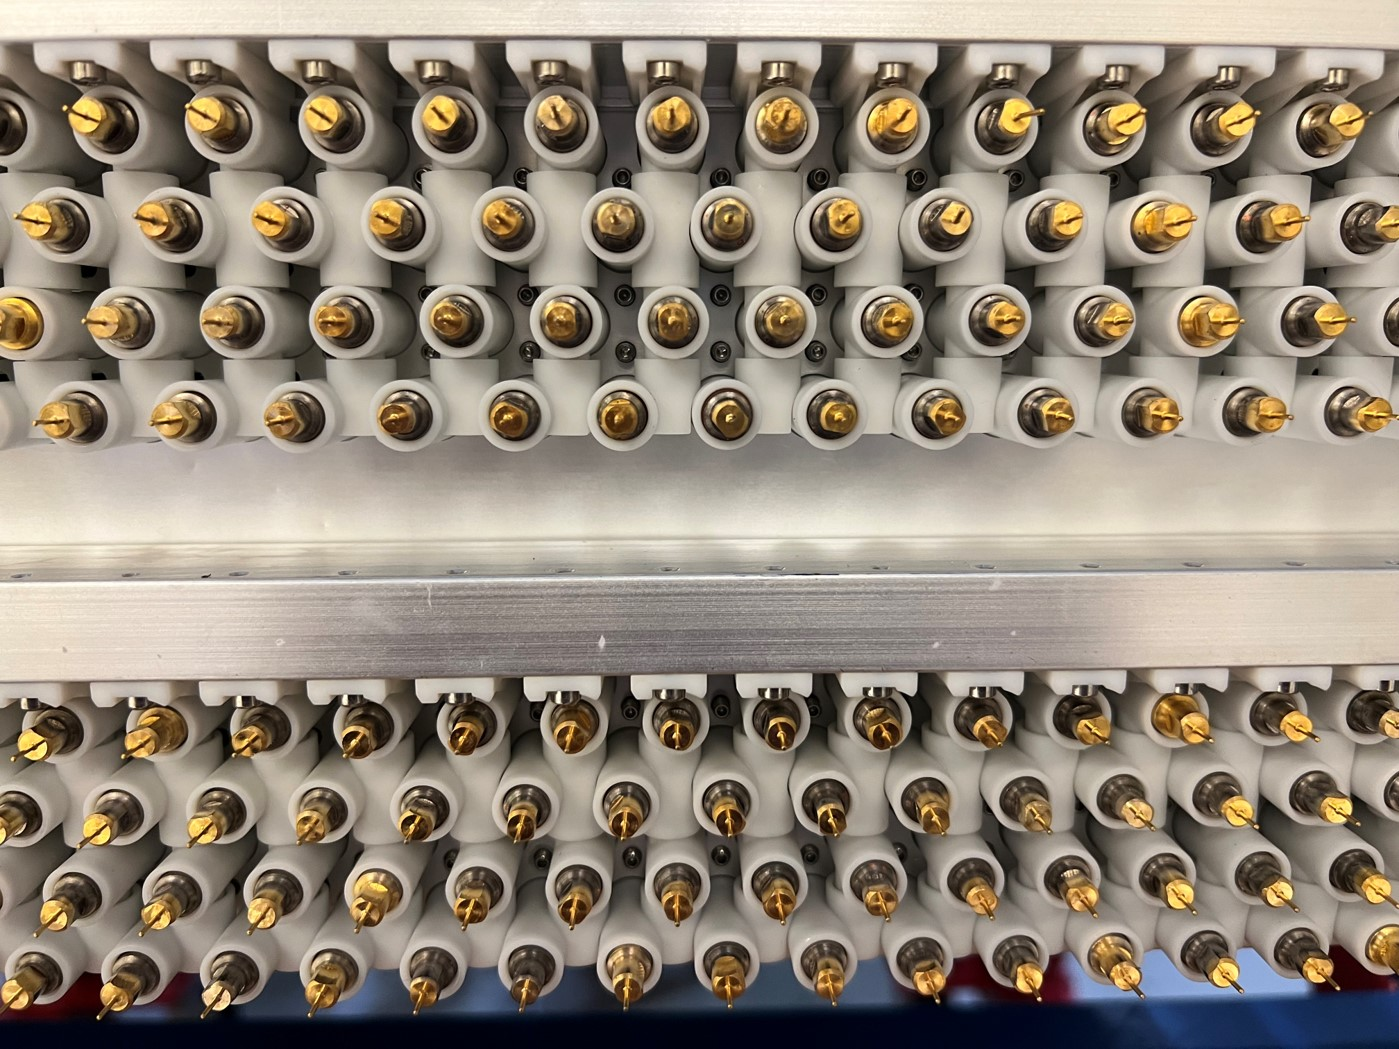
\includegraphics[width=0.39\linewidth]{figures/ch7-sMDT/gas-bar-signal-cap.jpg}}
\caption{(a) Pre-assemble gas bar. (b) Installation of a gas bar on chamber. (c) End view of a chamber with gas system and signal caps installed.}
    \label{fig:sMDT-gas-installation}
\end{figure}

The sMDT gas distribution system uses molded plastic fittings, shown in 
Figure~\ref{fig:sMDT-gas-installation}(a), which connects in sets of four to supply gas in series to four tubes arranged vertically across the four tube layers of a multilayer (ML).

On each side of an ML, two gas bars are connected to provide parallel gas flow into and out of the multilayer. The gas inlet and outlet are located at opposite corners to balance the flow impedance and ensure uniform gas distribution among all tubes. Gas enters the tube stacks through 1~mm diameter holes in the gas-bar manifolds.

%Early tests revealed that metal chips from machining could remain trapped in these small holes, partially blocking the gas flow to a group of four tubes. To prevent this, the gas bars are thoroughly cleaned and inspected before pre-assembly.

Figure~\ref{fig:sMDT-gas-installation}(b) shows the installation of the gas bars by two operators. An end view of a chamber with the gas bars and signal caps fully installed is shown in Figure~\ref{fig:sMDT-gas-installation}(c).

%%%%%%%%%

The ATLAS muon chamber upper limit on the leak rate is
\[
1\times10^{-5}\,[\mathrm{mbar \, L/s}] \times (2\,N_{\text{tube}}),
\]
where $2N_{\text{tube}}$ denotes the total number of endplugs included in the measurement.

The gas volume of an sMDT tube is approximately $V_{\text{tube}} \approx 250~\mathrm{cm^3}$.
Therefore, the volume of one multilayer (ML) is
\[
V_{\mathrm{ML}} = N_{\text{tube}} \times 250~\mathrm{cm^3}.
\]
Using this relation, the leak-rate limit can be converted to a corresponding limit on the chamber pressure drop during measurements. For an sMDT multilayer, this corresponds to a maximum pressure drop of $0.288~\mathrm{mbar/hour}$.

Because the chamber pressure depends on gas temperature, the measured pressure change ($\Delta P$) over a time interval ($\Delta t$) must be corrected for temperature variations before comparison with the leak-rate specification. The normalized leak rate is defined as
\begin{equation}
\label{eqn:LeakR8}
\left(\frac{\Delta P}{\Delta t}\right)_{\text{norm}} =
\frac{\Delta P_{\text{corr}}}{\Delta t},
\end{equation}
where the temperature-corrected pressure change is
\[
\Delta P_{\text{corr}} =
P_f \frac{T_{\text{ref}}}{T_f} -
P_i \frac{T_{\text{ref}}}{T_i}.
\]
Here $P_i$, $P_f$, $T_i$, and $T_f$ are the initial and final pressure and temperature, and $T_{\text{ref}} = 293.15~\mathrm{K}$ is the reference temperature.

For the measurements, the chamber gas outlet valves are connected to a precision pressure gauge (Figure~\ref{fig:leak-rate}(a)) that monitors the pressure of each ML. The chamber is pressurized with helium, and a helium sniffer is used to locate leaks at connection points or individual tubes. Most leaks can be repaired by replacing O-rings, gas stacks, or signal caps. If a tube leak cannot be repaired, the wire is removed, the end-plugs are sealed to isolate the tube from the gas system, and the signal caps are modified to isolate the tube from both the HV and RO electronics.

The chamber gas leak rates were measured multiple times at UM and at CERN.
The final leak-rate measurement is performed after installation of all the front-end electronics cards and Faraday cages and is shipped to CERN. The measured ML leak rates of the sMDT chambers constructed at UM are shown in Figure~\ref{fig:leak-rate}(b). The dashed line indicates the specification limit, while the blue (red) triangles represent the measured leak rates for ML1 (ML2). All measured values are well below the allowed limit.

\begin{figure}[!htbp]
    \centering
    \subfloat[]{
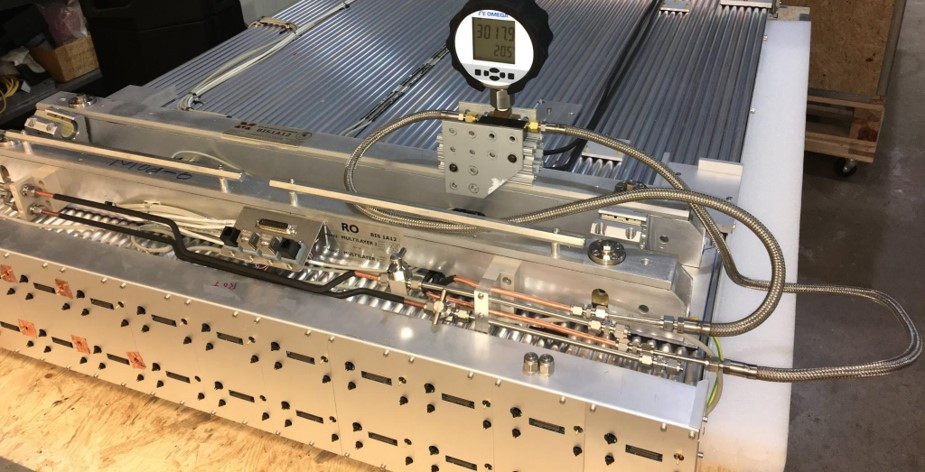
\includegraphics[width=0.465\linewidth]{figures/ch7-sMDT/gas-gauge-tubing.jpg}}
    \subfloat[]{
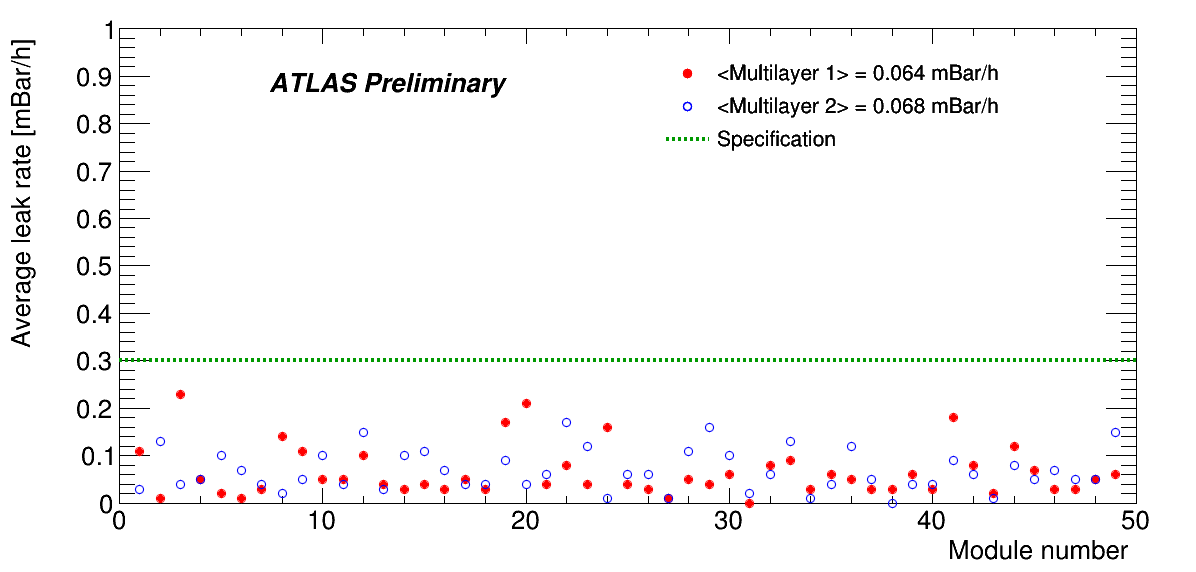
\includegraphics[width=0.525\linewidth]{figures/ch7-sMDT/sMDT-leakrate.png}}
\caption{(a) Chamber gas connections and precision pressure gauge used for leak-rate measurements. (b) Measured gas leak rates for each multilayer of the 50 sMDT chambers. All values are below the specified limit.}
    \label{fig:leak-rate}
\end{figure}


%%%%%%%%%%%%%%%%%%%%%%%%%%%
\subsection{Chamber performance test using cosmic-rays}

The final chamber performance is evaluated using cosmic-ray tests. 
For stable chamber operation, the grounding scheme follows a ``star'' design 
(see Figure~\ref{fig:grounding-chamber}) to avoid ground loops and minimize electronic noise.
\begin{figure}[!htbp]
    \centering
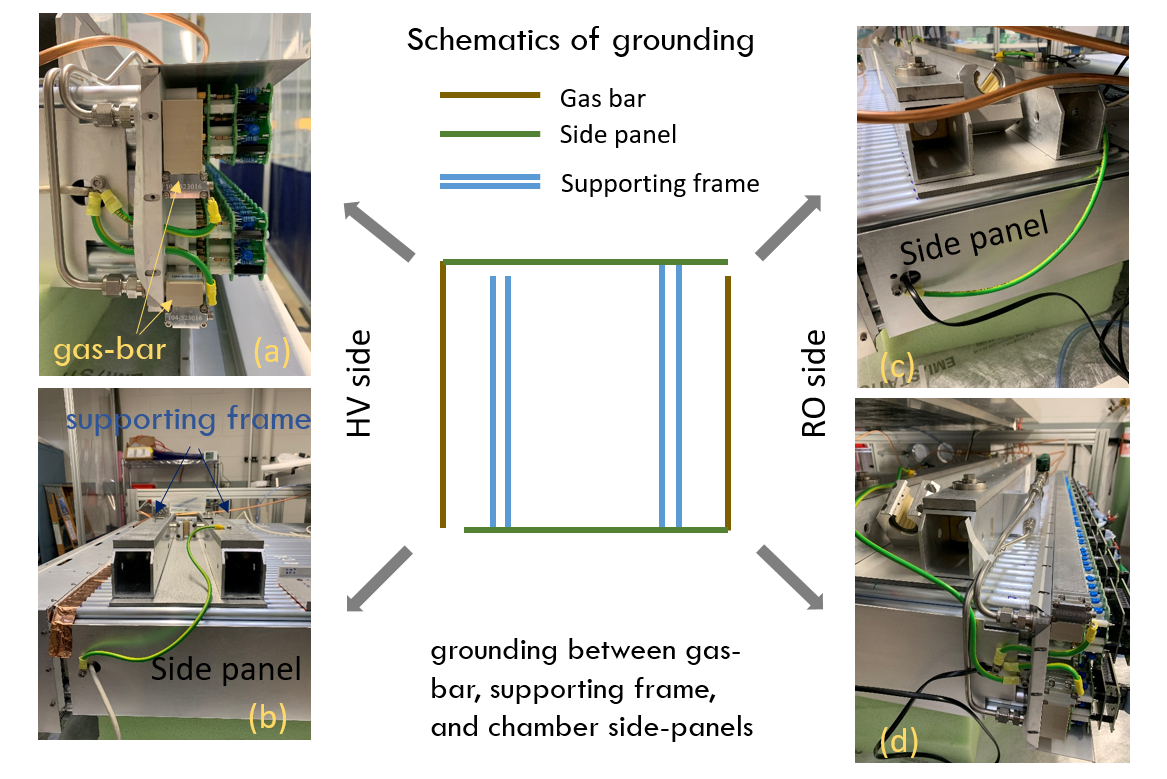
\includegraphics[width=0.98\linewidth]{figures/ch7-sMDT/Grounding.PNG}    
\caption{Schematic of the chamber grounding scheme and electrical connections.} 
    \label{fig:grounding-chamber}
\end{figure}
All tube walls are electrically connected to grounding foils that cover the tube ends 
and are connected to the Faraday cages. External structures, including the gas bars, 
support structure, and chamber side panels, are electrically isolated from the tube walls. 
These components are instead connected in a star configuration to the foil ground, 
as illustrated in the schematic in the center of Figure~\ref{fig:grounding-chamber},
and the pictures from (a) to (d) show the connections of the grounding cables between gas-bar, support frame, and chamber side-pannel.


The schematic of the electrical connections to a drift tube is shown in Figure~\ref{fig:Elx-chamber}(a). 
For an sMDT tube, the 383~$\Omega$ resistor on the HV side shown in the figure is replaced by a 330~$\Omega$ resistor.

The readout (RO) and high-voltage (HV) hedgehog (HH) cards consist mainly of passive components and are mounted directly onto the signal and ground pins through sockets on the cards. A double-stack mezzanine card is installed on top of the RO HH cards, as shown in Figure~\ref{fig:Elx-chamber}(b).

\begin{figure}[!htbp]
    \centering
    \subfloat[]{
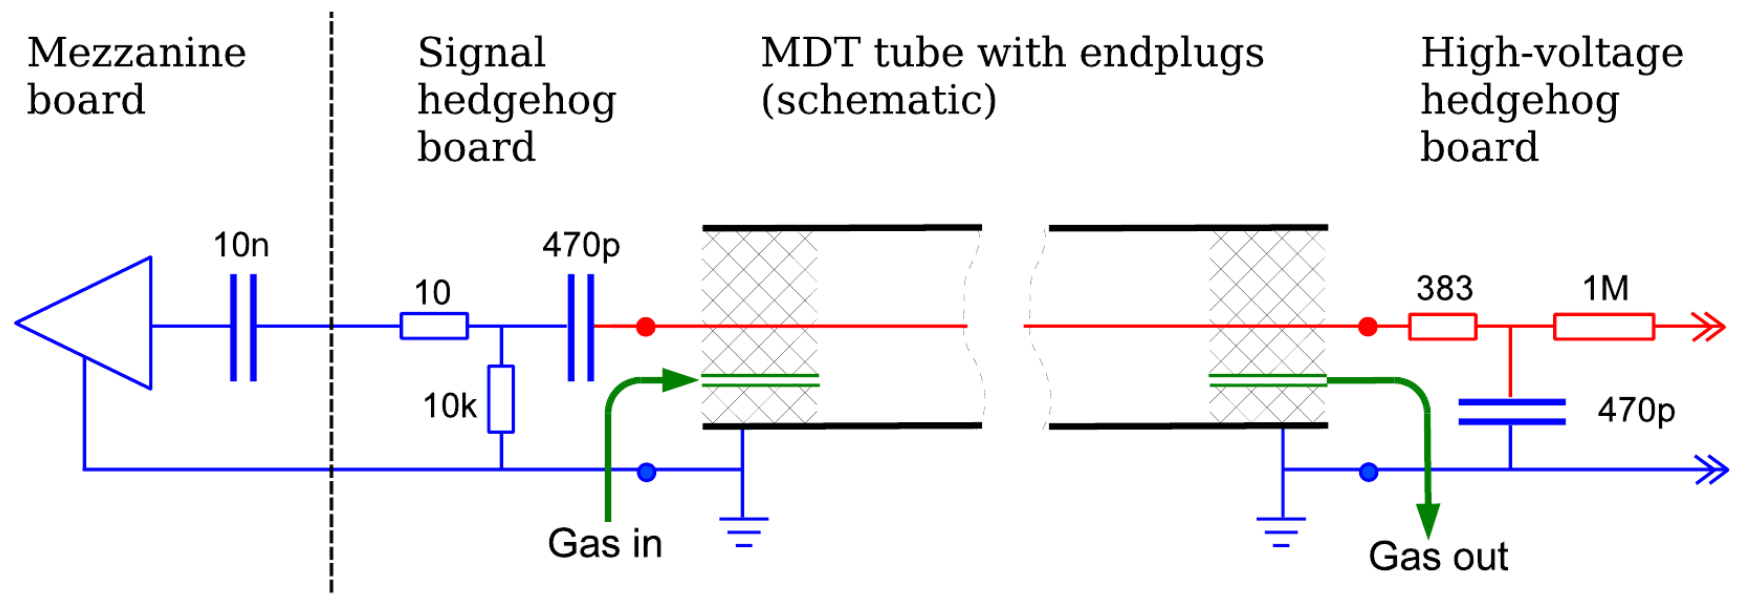
\includegraphics[width=0.60\linewidth]{figures/ch7-sMDT/ElectricalConnection.PNG}}
\hspace{0.1cm}
    \subfloat[]{
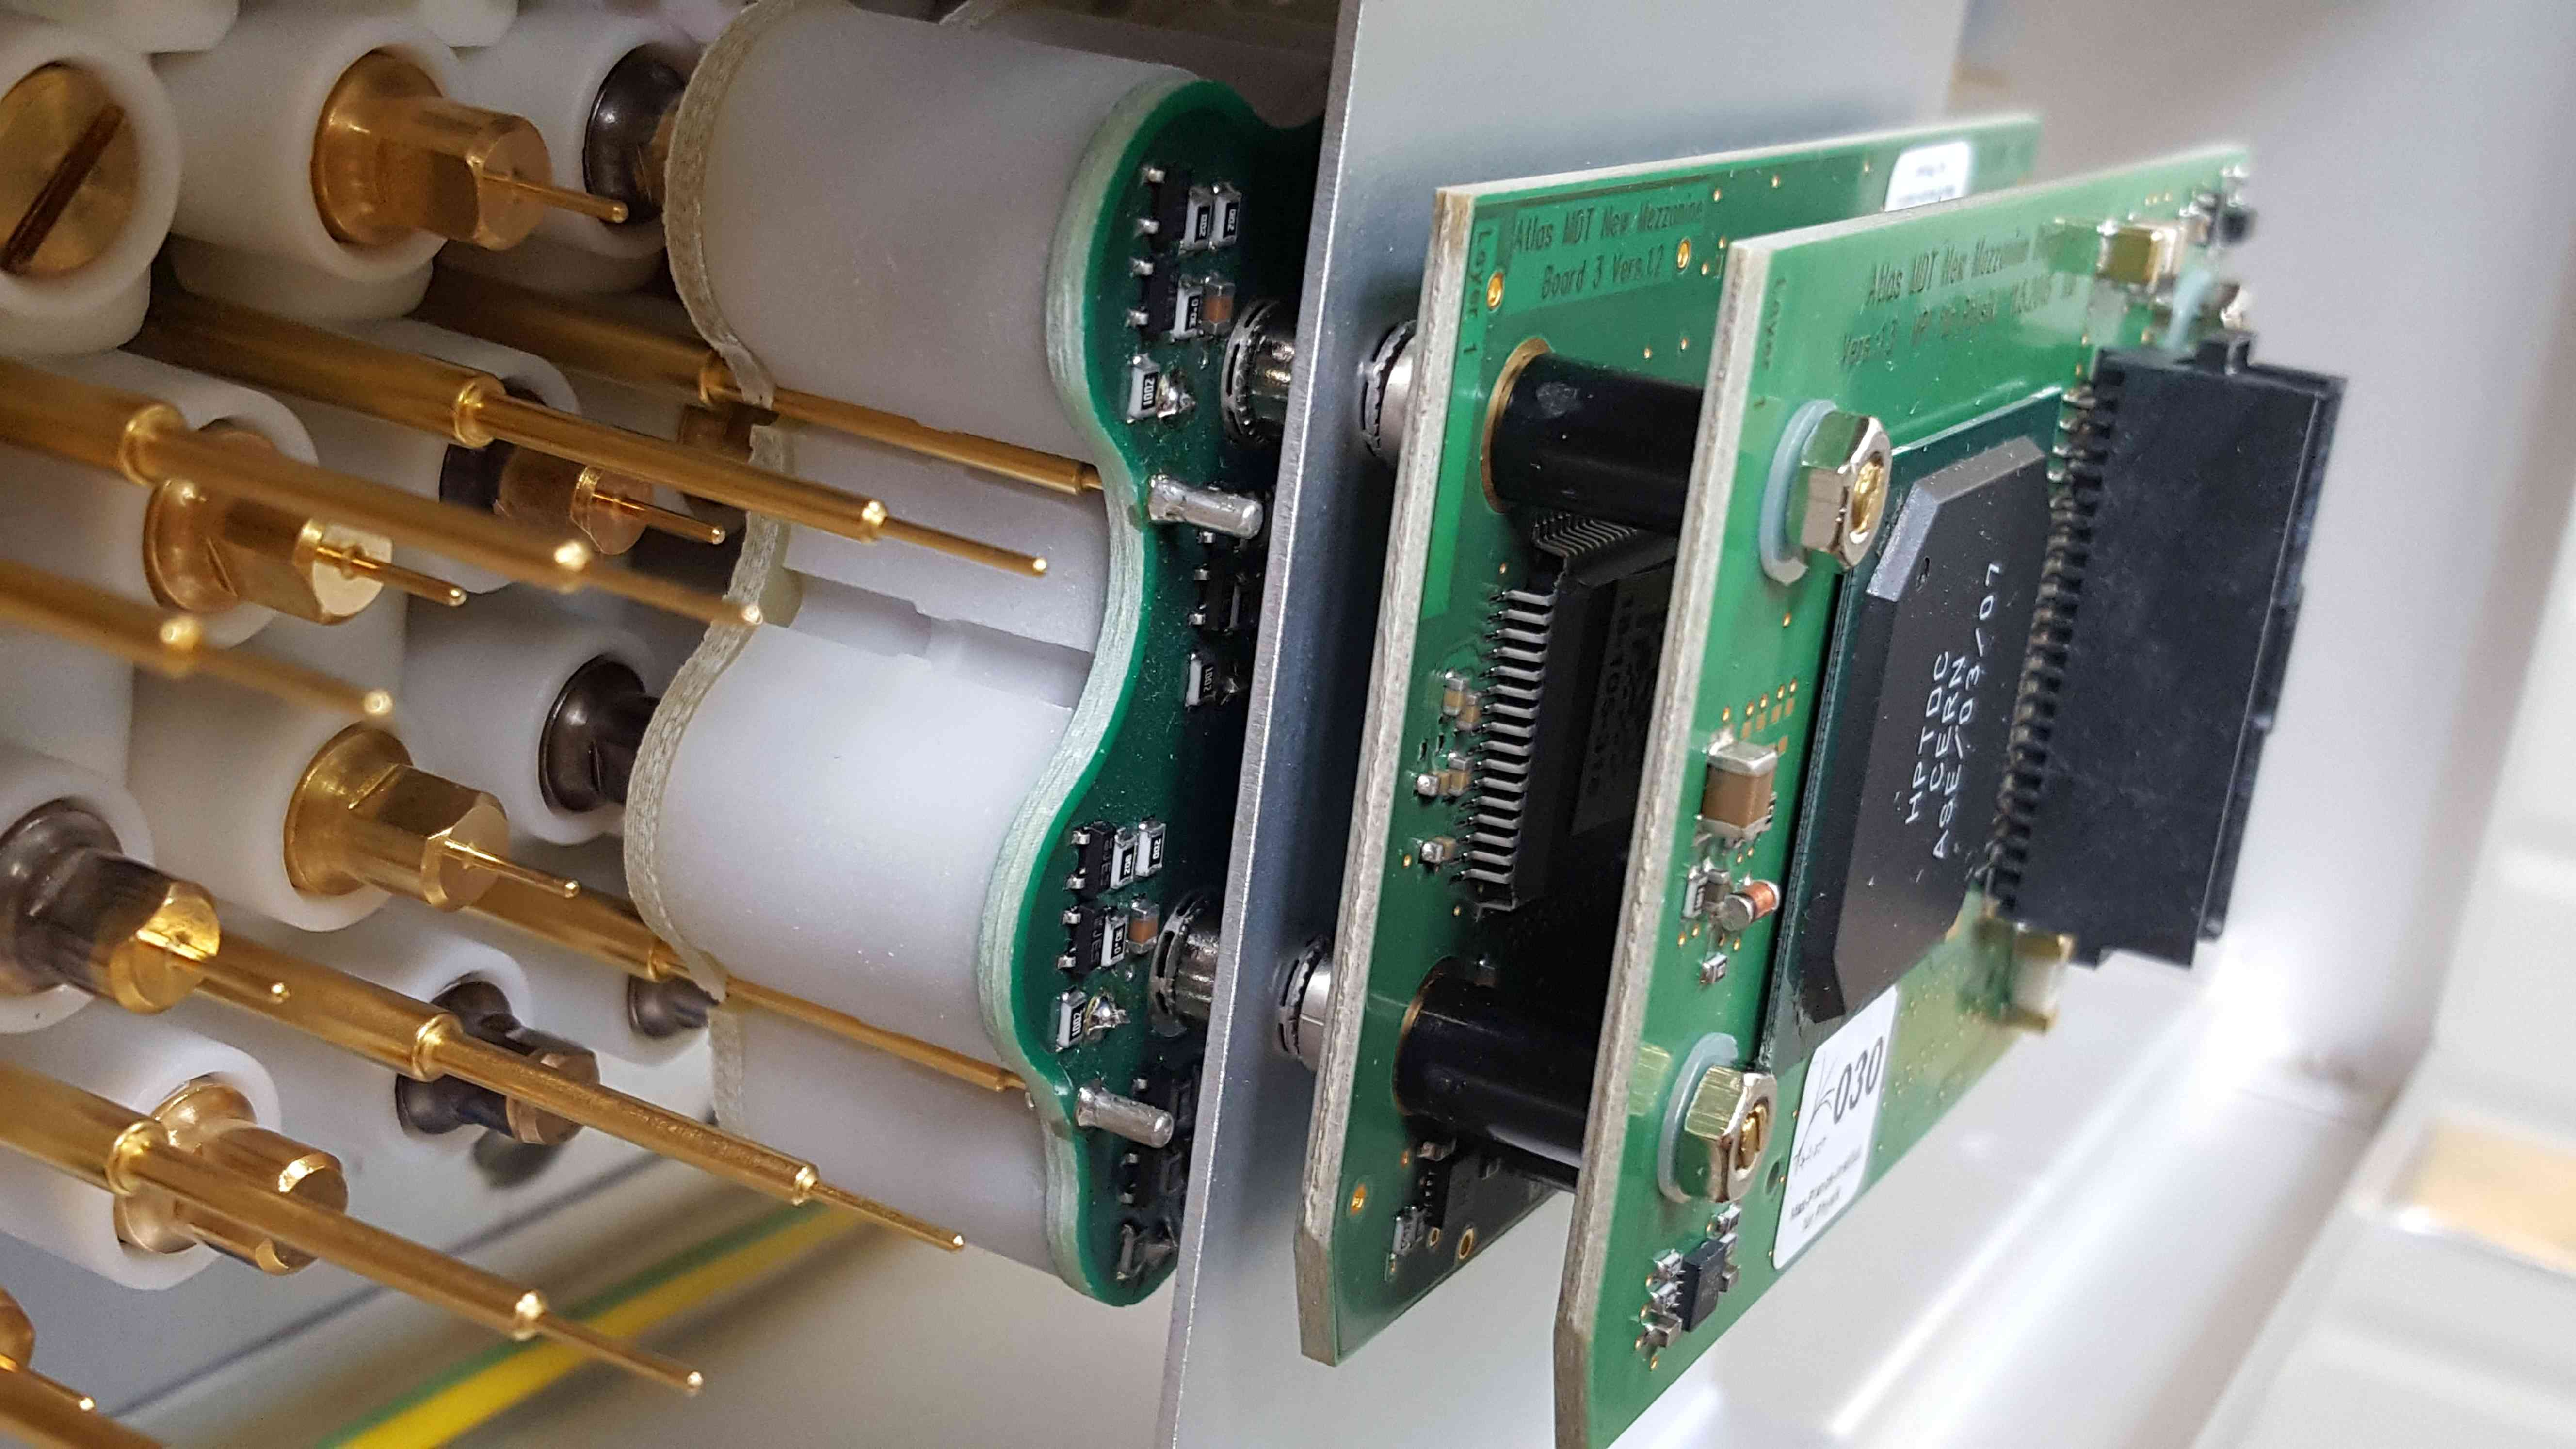
\includegraphics[width=0.35\linewidth]{figures/ch7-sMDT/ATLAS-TDR-026.jpg}}
\caption{(a) Schematic of the electrical connections to a drift tube. (b) The RO HH card is connected to the tube signal and grounding pins, with the readout mezzanine card mounted on top.}
    \label{fig:Elx-chamber}
\end{figure}

A cosmic-ray test station, consisting of a gas control panel, scintillator trigger detectors, and HV and LV power supplies, is installed in a humidity-controlled test laboratory. The test chamber is mounted on a custom-built mobile chamber cart, as shown in Figure~\ref{fig:cosmic-station}(a). An end view of a chamber on the test station connected to 24 mezzanine cards and cables is shown in Figure~\ref{fig:cosmic-station}(b).

A schematic of the data acquisition (DAQ) system is shown in Figure~\ref{fig:cosmic-daq}(a). The DAQ system (Figure~\ref{fig:cosmic-daq}(b)) is located outside the humidity-controlled test room and includes two computers: a Windows computer for DAQ configuration and control, and a Linux computer for data taking. The system also contains a VME crate with the DAQ interface and trigger modules, HV power supplies for the chamber and trigger scintillators, and a NIM crate for trigger coincidence logic.

The DAQ firmware and the software for online data monitoring were developed at Michigan. During the cosmic-ray tests, reconstructed muon tracks, tube hit maps, and ADC and TDC spectra for each sMDT tube are displayed online.

\begin{figure}[!htbp]
    \centering
    \subfloat[]{
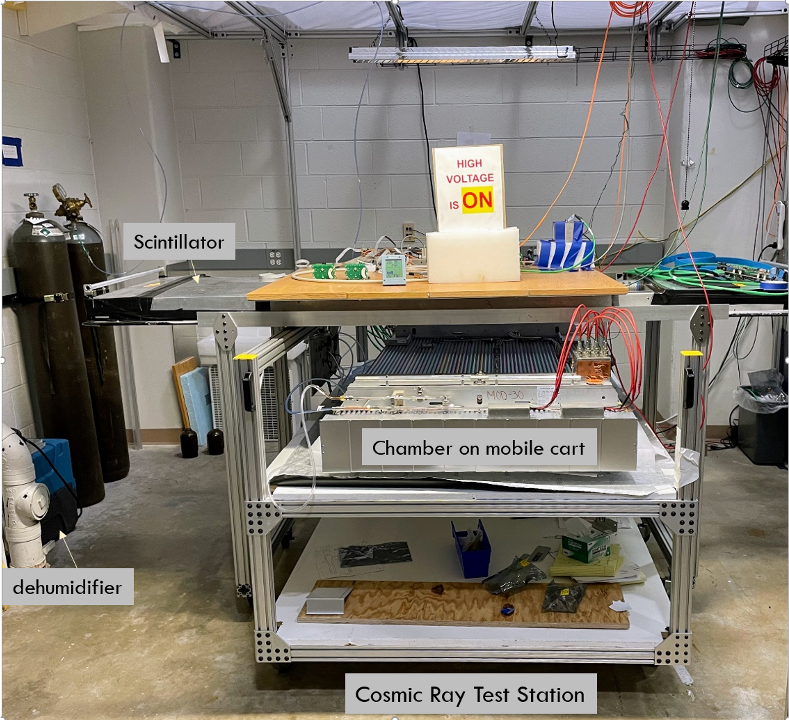
\includegraphics[width=0.32\linewidth]{figures/ch7-sMDT/CosmicRay-Station.PNG}}
    \subfloat[]{
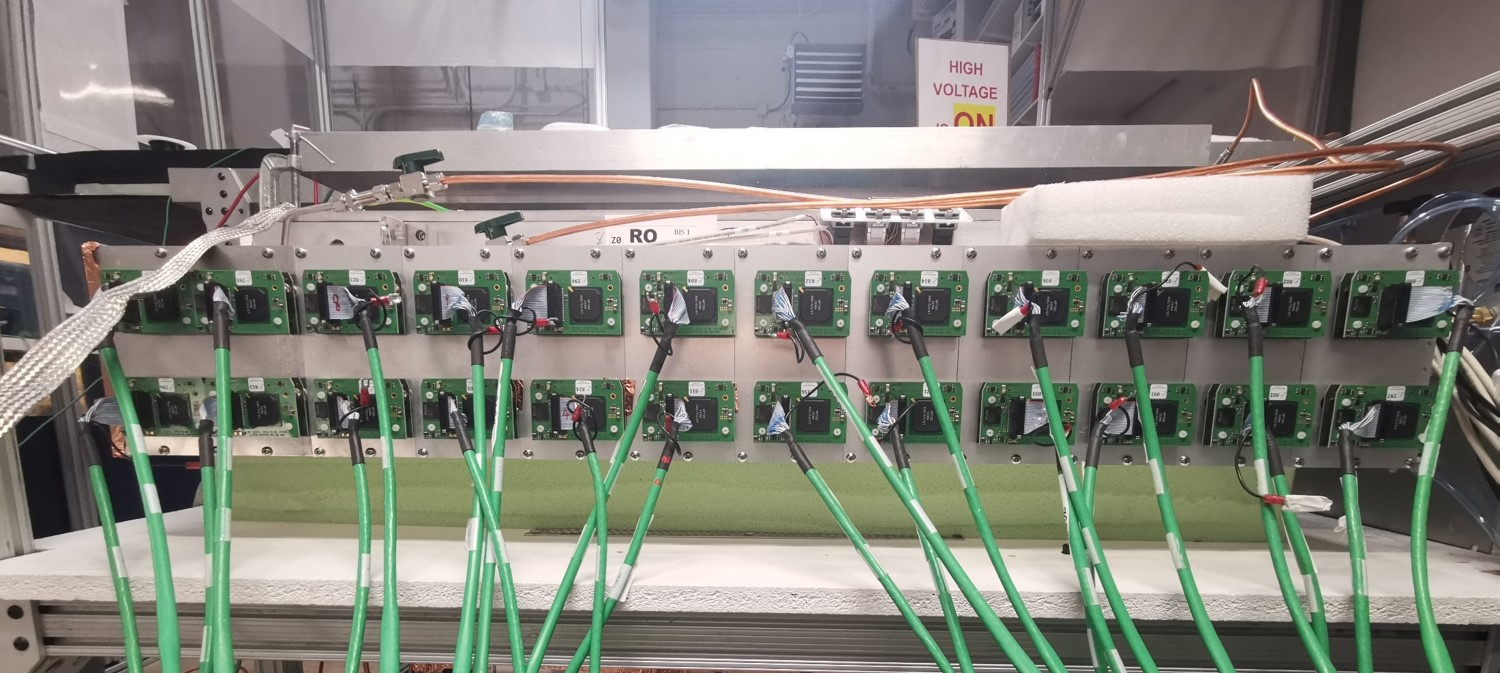
\includegraphics[width=0.65\linewidth]{figures/ch7-sMDT/RO-side.jpg}}
\caption{(a) Cosmic-ray test station. (b) End view of a chamber connected to 24 mezzanine cards and cables for the cosmic-ray test.}
    \label{fig:cosmic-station}
\end{figure}

\begin{figure}[!htbp]
    \centering
    \subfloat[]{
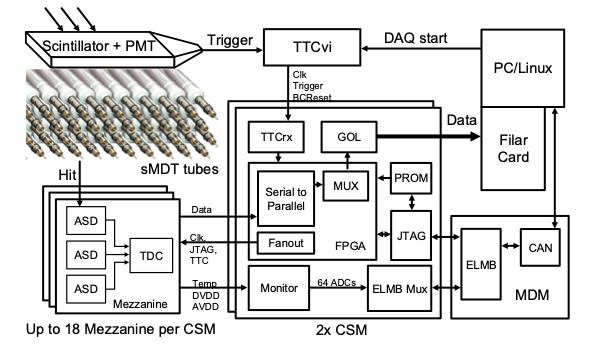
\includegraphics[width=0.58\linewidth]{figures/ch7-sMDT/DAQ_Diagram.png}}
    \subfloat[]{
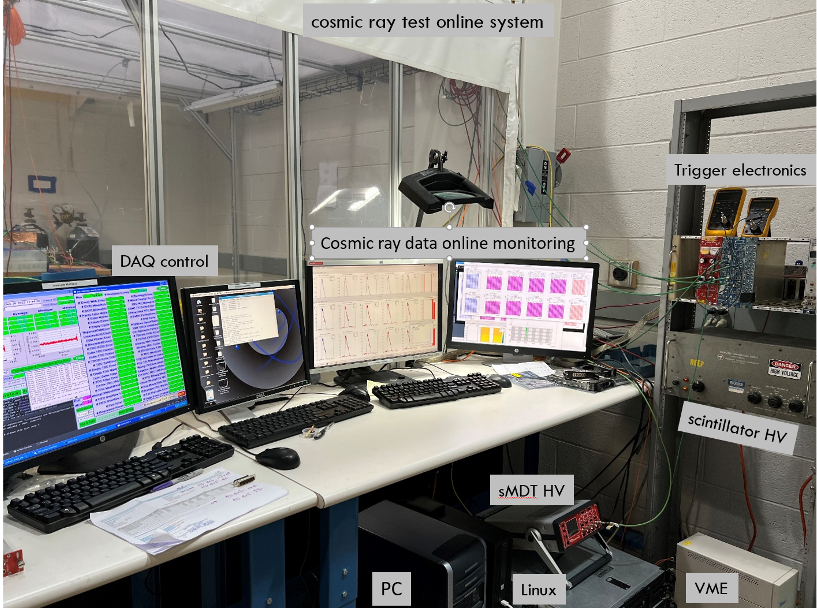
\includegraphics[width=0.40\linewidth]{figures/ch7-sMDT/Cosmic-DAQ-system.PNG}}
\caption{Cosmic-ray test DAQ system: (a) schematic of the DAQ architecture; (b) DAQ hardware setup.}
    \label{fig:cosmic-daq}
\end{figure}

To prepare the chamber for noise measurements and cosmic-ray tests, it is conditioned by a three-day burn-in period with a gas flow rate of 3 volumes per day, and with both HV and LV applied to the chamber and front-end electronics. Channels exhibiting elevated noise are treated by applying negative HV for several hours to reduce the noise level. For some tubes located at the chamber corners, improved grounding is achieved by tightening the grounding connections.

The noise rate of each tube is measured in a series of runs at different readout thresholds with both HV off and HV on (at the nominal operating voltage of +2730~V). 
A 10~kHz pulse generator provides the trigger for reading out noise hits.

The noise rate is calculated from the recorded number of hits and triggers during the data-taking period (typically $\Delta t = 10$ minutes):
\begin{equation}
\text{Noise rate} =
\frac{N_{\text{hits}}}{N_{\text{trigger}} \times t_{\text{window}}},
\end{equation}
where $t_{\text{window}} = 1.55~\mu$s is the TDC readout time window, $N_{\text{hits}}$ is the number of hits recorded in a channel during the test interval $\Delta t$, and
$N_{\text{trigger}} = 10~\text{kHz} \times \Delta t$.

The measured average noise rate per tube for HV off and on at a readout threshold of $-27$~mV is shown in Figure~\ref{fig:noise} for all 50 sMDT chambers constructed at Michigan. 
The observed noise rate of about 20~Hz per tube is approximately five times lower than the specification limit of 100~Hz per tube.

\begin{figure}[!htbp]
    \centering
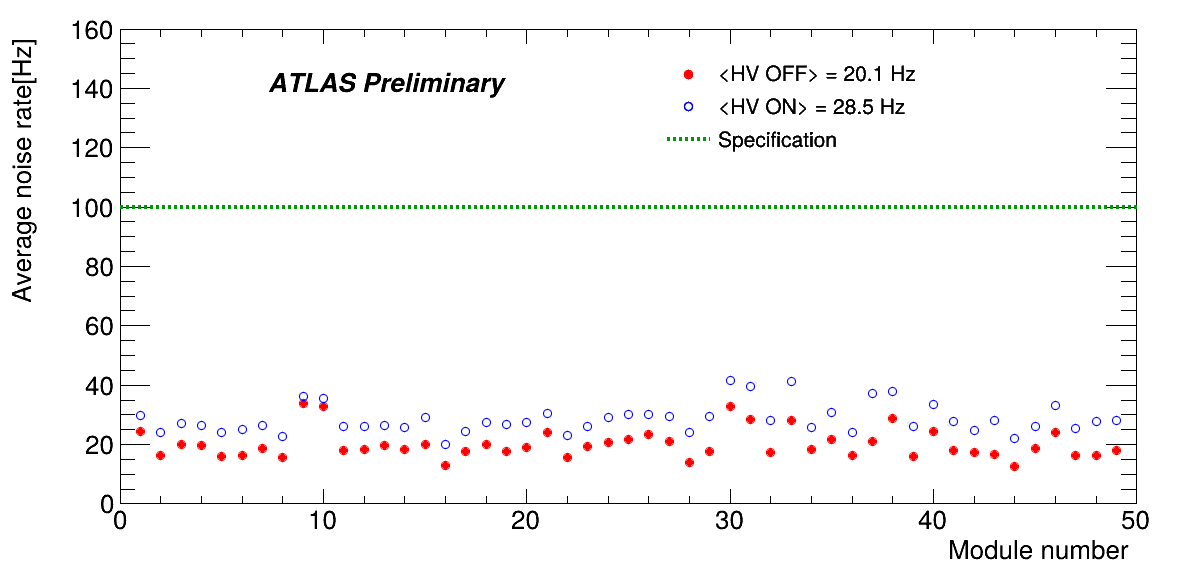
\includegraphics[width=0.95\linewidth]{figures/ch7-sMDT/sMDT-noise.png}    
\caption{Measured noise rates for all 50 sMDT chambers constructed at UM.}
    \label{fig:noise}
\end{figure}

Each tube’s response to charged particles is tested using cosmic rays. 
Figure~\ref{fig:cosmic-data} shows typical raw data from a representative sMDT chamber: 
(a) the time (TDC) spectrum and (b) the charge (ADC) spectrum for tube hits. 
The leading and trailing edges of the TDC distribution are fitted with Fermi–Dirac functions to determine the time offset ($T_0$) and the maximum drift time ($T_{\mathrm{max}}$). 
The ADC distribution is fitted with a skew-normal function. 
The measured drift time for each hit, defined as the difference between the hit time and $T_0$, is corrected for time-slewing using the charge information. 
Time-slewing arises from the jitter introduced by variations in the time at which signals with different amplitudes cross the ASD threshold.

This time-to-space relationship (also called RT-function), shown in Figure~\ref{fig:cosmic-data}(c), is obtained with an auto-calibration program that converts the drift time to the drift distance through a procedure of minimizing the tracking residuals of all the collected muon tracks in a test run.

\begin{figure}[!htbp]
    \centering
    \subfloat[]{
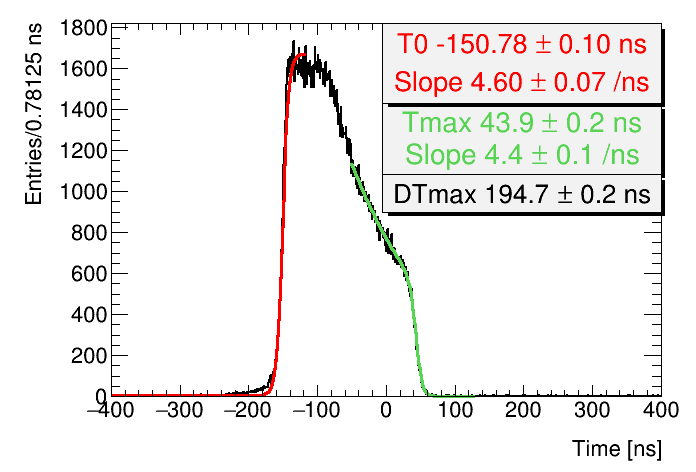
\includegraphics[width=0.325\linewidth]{figures/ch7-sMDT/sMDT-TDC_fit.png}}
    \subfloat[]{
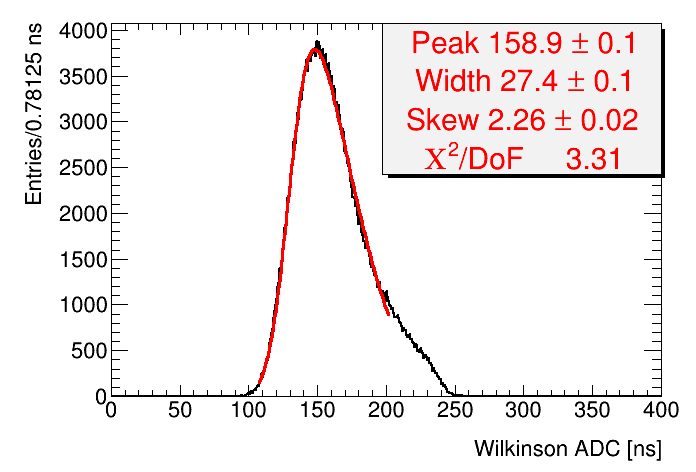
\includegraphics[width=0.325\linewidth]{figures/ch7-sMDT/sMDT-ADC_dist.png}}
    \subfloat[]{
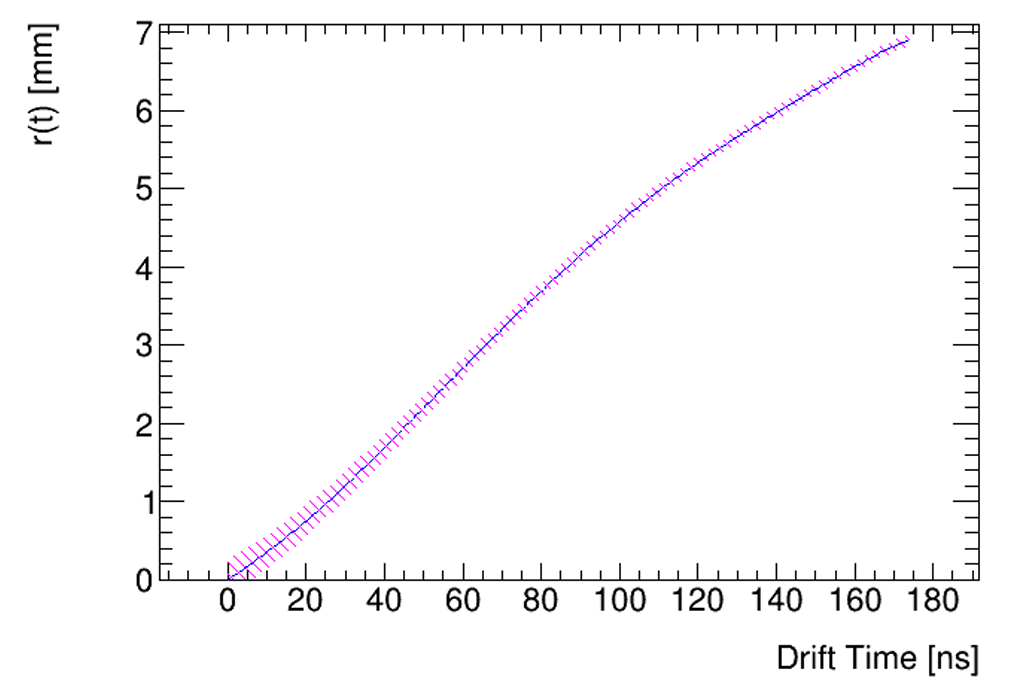
\includegraphics[width=0.33\linewidth]{figures/ch7-sMDT/sMDT-RT-function.png}}
\caption{Cosmic-ray test data for a representative sMDT tube: (a) TDC spectrum, (b) ADC spectrum, and (c) the derived RT function.}
    \label{fig:cosmic-data}
\end{figure}

An example of a cosmic-ray muon track reconstructed in an sMDT chamber built at UM is shown in Figure~\ref{fig:display}(a). 
The muon track is reconstructed by fitting a line tangent to the drift circles (shown in blue in the event display). 
Grey (white) circles correspond to drift tubes read out by a different (the same) mezzanine card.

The single-tube spatial resolution is determined from the residual distributions obtained by fitting reconstructed muon tracks. 
The tracking residual is defined as
\[
r_{\mathrm{drift}} - r_{\mathrm{fit}},
\]
where $r_{\mathrm{drift}}$ is the measured drift radius and $r_{\mathrm{fit}}$ is the radius predicted by the fitted track.

Two types of residuals are used: biased and unbiased. 
The biased residual is obtained when the track is fitted using all hits. 
The unbiased residual is calculated by removing the hit under study from the track fit and evaluating its residual with respect to the refitted track. 
Figures~\ref{fig:display}(b) and (c) show the corresponding biased and unbiased residual distributions.

\begin{figure}[!htbp]
    \centering
    \subfloat[]{
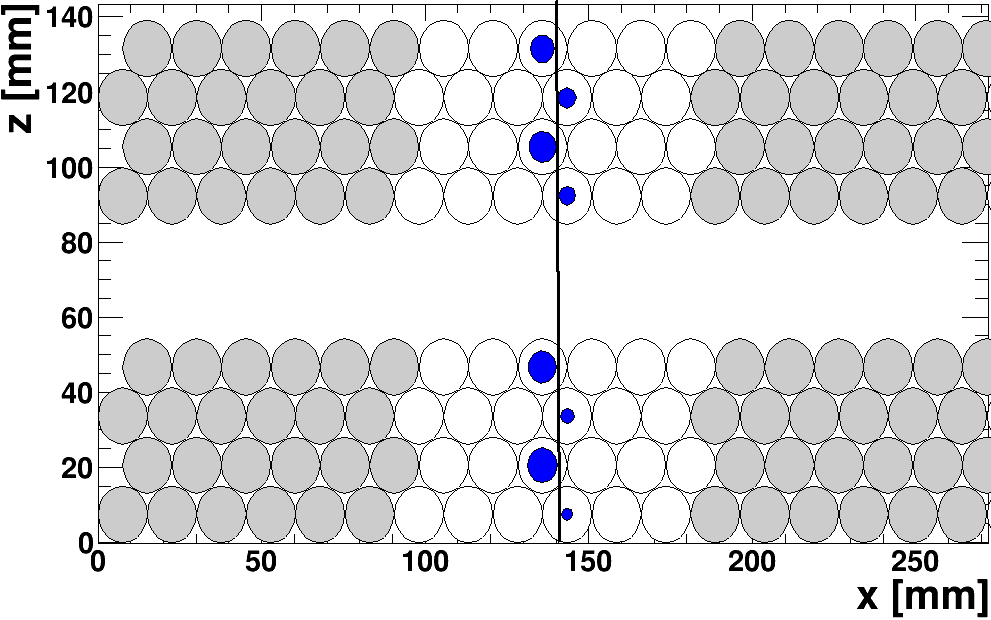
\includegraphics[width=0.35\linewidth]{figures/ch7-sMDT/BIS_track.png}}
    \subfloat[]{
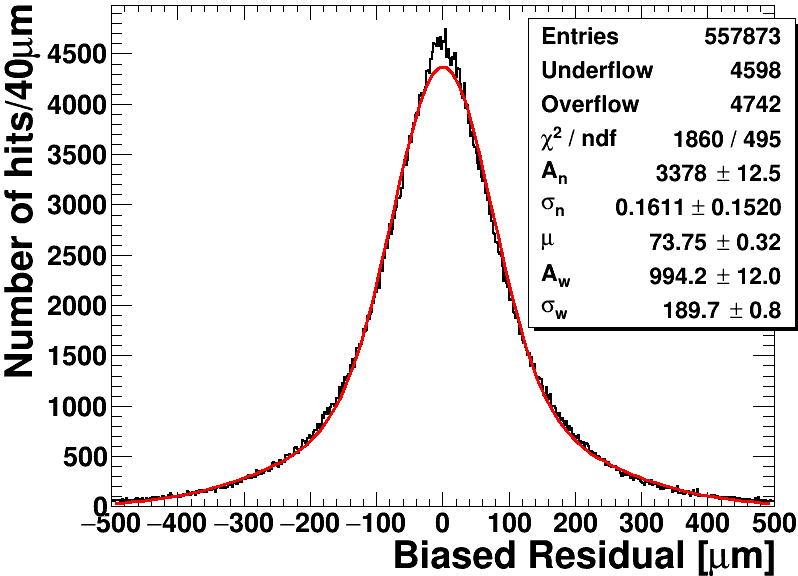
\includegraphics[width=0.31\linewidth]{figures/ch7-sMDT/Module14_BiasedResidual.png}}
    \subfloat[]{
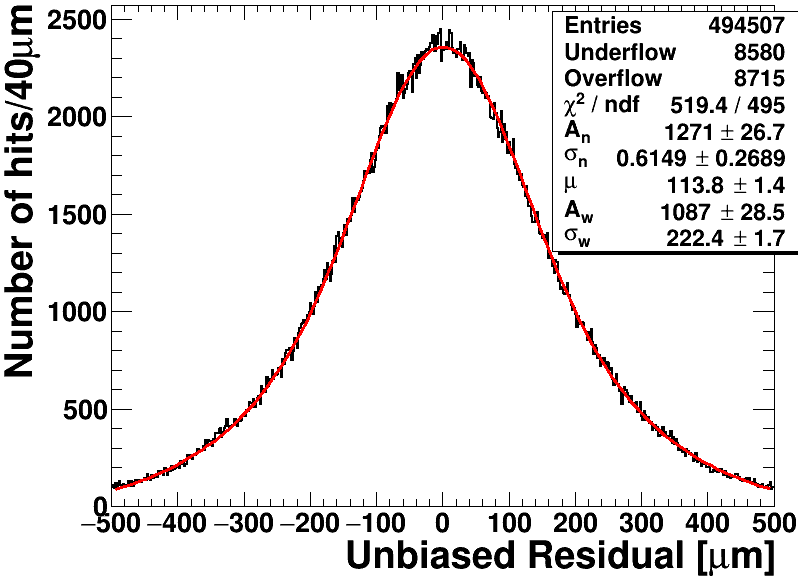
\includegraphics[width=0.31\linewidth]{figures/ch7-sMDT/Module14_UnbiasedResidual.png}}
\caption{Cosmic-ray test results: (a) example event display with a reconstructed muon track and drift circles; (b) biased residual distribution; (c) unbiased residual distribution.}
    \label{fig:display}
\end{figure}

A residual distribution is fitted with a double Gaussian function with a common mean
and the single wire resolution is defined as:
\begin{equation}
\sigma_{wire} = \sqrt{ \, \sigma_{B}^{} \cdot \sigma_{U}^{}\, }
\end{equation}
where $\sigma_{B}^{} \; (\sigma_{U}^{}) $ is the biased (unbiased) residual width calculated as 
amplitude weighted average of the two Gaussian components, narrow ($n$) and wide ($w$), of the fit:
\begin{equation}
\sigma_\alpha = \frac{ A_{n} \cdot \sigma_{n} + 
                   A_{w} \cdot \sigma_{w} }{ A_{n} + A_{w} }, \hspace{1cm} (\alpha=B, \ U).
\end{equation}

The measured single-tube spatial resolutions for all 50 sMDT chambers are shown in Figure~\ref{fig:resolution} for readout thresholds of $-27$~mV and $-39$~mV. The measured resolutions, all below $90~\mu$m, are well within the specification of $106~\mu$m. Maintaining a low chamber noise level is essential for achieving optimal tracking resolution.

The tube-layer efficiency is defined as the ratio of the number of hits in that layer associated with reconstructed tracks to the number of tracks passing through the layer. This efficiency includes the intrinsic tube efficiency as well as inefficiencies arising from the tube walls and the gaps between tubes (dead regions).
%4480 BIS1 (70x8LYx8sMDT) + 10208 BIS2-6(58x8LYx22sMDT)
%Out of the 14688 tubes of the first 30 UM sMDT chambers, 13 were lost due to wire slippage (insufficient crimping) or irreparable gas leaks (cracked endplug or improper endplug swaging).
Figure~\ref{fig:eff} shows the tube-layer efficiency averaged over a chamber (referred to as the tracking efficiency) for all 50 chambers built at Michigan. The average tracking efficiency for each tube layer is $94.70 \pm 0.03$~\%.
\begin{figure}[!htbp]
    \centering
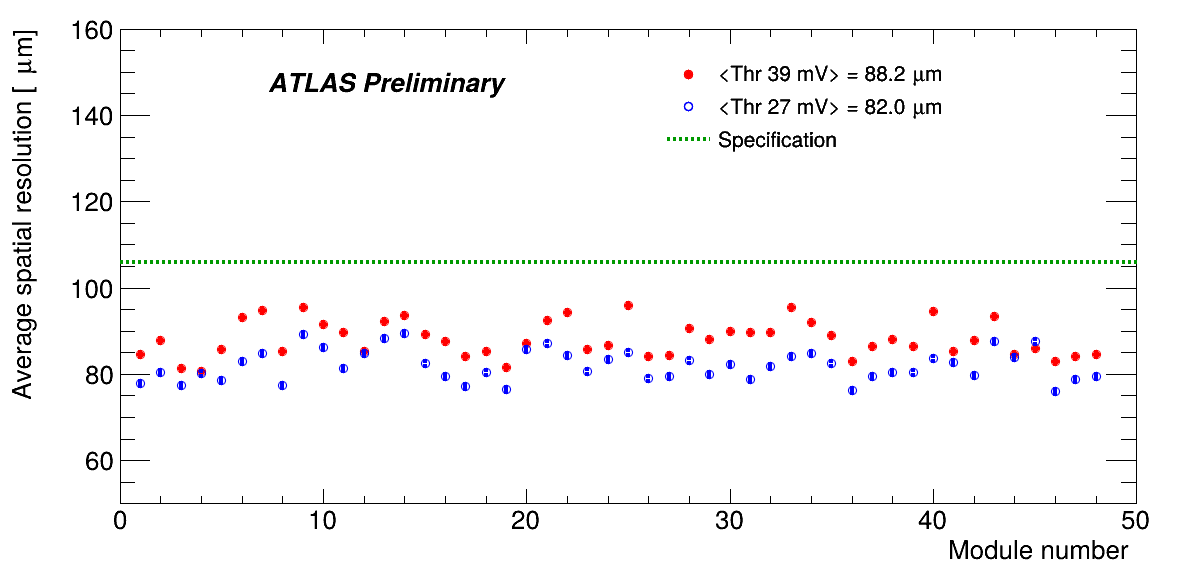
\includegraphics[width=0.95\linewidth]{figures/ch7-sMDT/sMDT-resolution.png}    
\caption{The measured tracking resolution per tube for all 50 sMDT chambers built at UM.} 
    \label{fig:resolution}
\end{figure}

\begin{figure}[!htbp]
    \centering
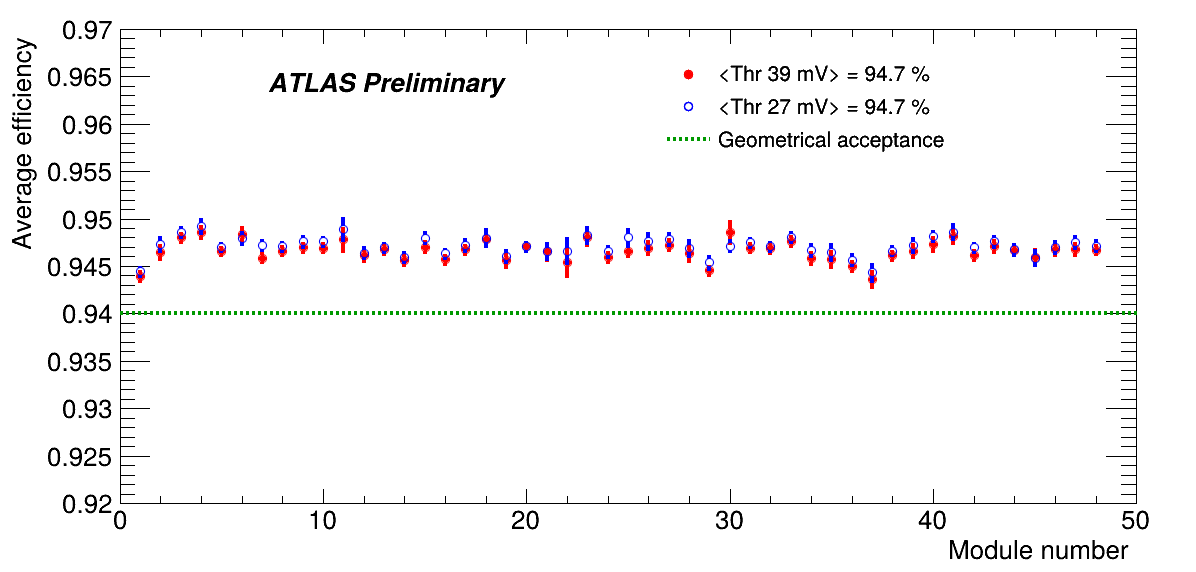
\includegraphics[width=0.95\linewidth]{figures/ch7-sMDT/sMDT-eff.png}    
\caption{The measured tracking efficiencies for all 50 sMDT chambers built at UM.} 
    \label{fig:eff}
\end{figure}

\section{Summary of the sMDT construction project}

A total of 26,000 precision drift tubes and 50 sMDT chambers were constructed and tested, meeting stringent quality-control requirements. This multi-year sMDT construction project involved tube production at Michigan State University, with tube testing and chamber assembly carried out at the University of Michigan. The effort was highly successful and represents a major contribution to the ATLAS muon spectrometer upgrade for the HL-LHC program. Figure~\ref{fig:sMDT-Team} shows the dedicated sMDT production team, including the author of this thesis.
\begin{figure}[!htb]
    \centering
 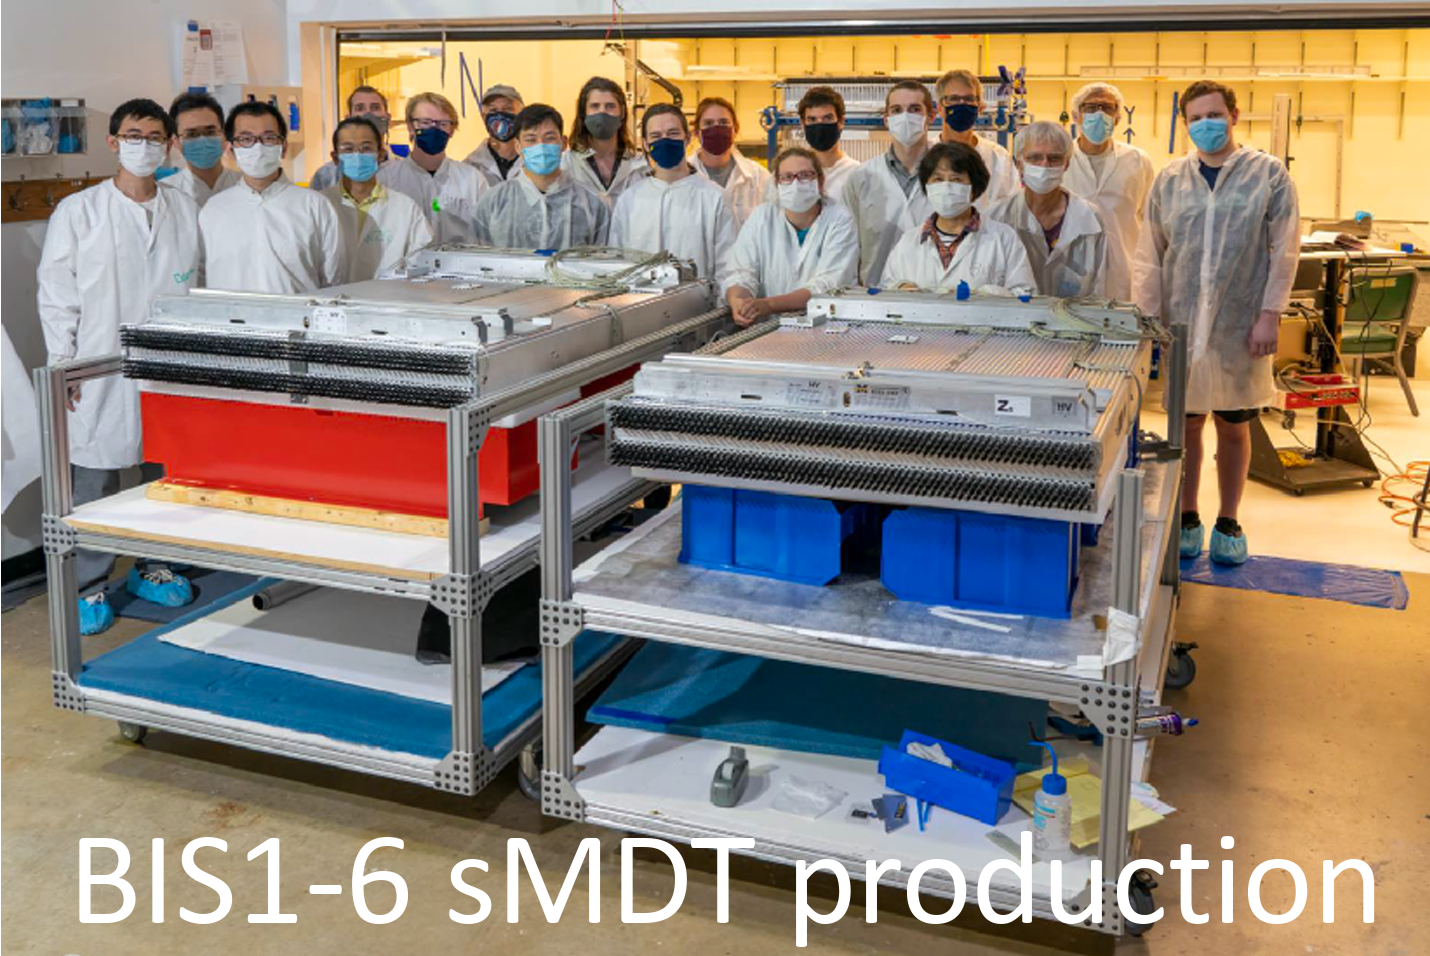
\includegraphics[width=0.8\linewidth]{figures/ch7-sMDT/sMDT-production-UM.png}
    \caption{The sMDT production team in the UM lab. Two constructed chambers are also shown in the picture. The 3rd person from the left is the author of this thesis.}
    \label{fig:sMDT-Team}
\end{figure}

This project required a multi-year R\&D effort to design and build the necessary infrastructure and construction tooling, as well as to construct two prototype chambers for developing the chamber assembly and testing procedures. The author played a major role in carrying out the intensive R\&D needed to prepare for large-scale chamber production, including contributions to multiple review processes at CERN and by the NSF.

Following the R\&D phase, sMDT chamber production began in mid-2020 and was completed by the end of 2023. All chambers were shipped to CERN by mid-2024 and were retested after shipping. Commissioning with the final electronics was carried out at CERN during 2024--2025.

Participation in and major contributions to this large-scale precision detector construction project have provided the author with invaluable experience as an experimental PhD student. Through this work, the author gained a deep understanding of what constitutes a precision detector and the processes required for its construction. These processes involve careful engineering design, high-precision machining, precise surveying, and detailed measurements. Each step relies on state-of-the-art hardware and associated software, reflecting modern technological developments and applications. The author also had opportunities to build hardware and develop software for detector construction, control, and testing.
%%%%%%%%%%%%%%%%%%
``Nothing is easy'' was a phrase often repeated by the construction team during detailed technical work, reflecting the challenges inherent in precision detector construction. Many unexpected problems arose, and solutions had to be developed throughout the construction steps. A few examples are given below.

\noindent\textbf{\bullet $\hspace{0.2 cm}$ Wire tension loss}:  
The wire tension is set using a calibrated gauge and measured with a custom circuit. During R\&D, the measured tension was ~100~g lower than expected. Investigations excluded gauge calibration and twisting resistance as causes. The issue was traced to the crimping tube not fully seated against the end plug, which shortened the wire by ~100~$\mu$m during crimping and reduced tension. The solution was to ensure operators held the crimping tube firmly against the end plug during assembly.

\noindent\textbf{\bullet $\hspace{0.2 cm}$ Tube leakage}:  
The tube gas seal is achieved by swaging the tube to compress the O-ring on the end plug using a custom-built swaging head with three rollers mounted on a spindle motor (see Figure~\ref{fig:sMDT-tubeswage}). Early in production, the gas-tightness failure rate was high. Measurements of O-ring compression in different orientations revealed asymmetric compression, indicating misaligned rollers after repeated use. The issue was corrected by inserting shims and performing frequent checks to ensure consistent swaging and proper gas-tightness.

\noindent\textbf{\bullet $\hspace{0.2 cm}$ Wire slippage}:  
Some wires slipped during assembly or later in chamber tests due to insufficient crimping to secure the wire on the tube (see Figure~\ref{fig:sMDT-wire-tension}). This issue was detected by measuring the crimped tube thickness: if it exceeded 0.7~mm, the wire could slip and contact the tube wall. The solution was to adjust the wire holders and implement a verification step to confirm proper tension after crimping.

\noindent\textbf{\bullet $\hspace{0.2 cm}$ Gas-flow hole blockage}:  
Blockages in the tube gas-flow holes were occasionally observed, caused by debris from the machining process. The problem was mitigated by introducing rigorous cleaning procedures and quality inspections before gasbar assembly.

\noindent\textbf{\bullet $\hspace{0.2 cm}$ Precision measurement of tube position}:  
Accurate tube placement was critical for chamber performance. Early measurements showed deviations beyond the specification from nominal positions. The main causes were height gauge calibration errors and small debris on the granite reference table used to measure tube height. The issue was resolved through repeated calibration and cleaning of the granite surface during construction.


%%%%%%%%%%%%%%%%%%
Finally, the fully tested sMDT chambers will be integrated with RPC detectors this year and installed in the ATLAS experiment during the LHC Long Shutdown~3, beginning at the end of June this year.